\documentclass{thesisclass}
% Based on thesisclass.cls of Timo Rohrberg, 2009
% ----------------------------------------------------------------
% Thesis - Main document
% ----------------------------------------------------------------
% No empty in-between chapters, remove this line if desired for double-page printing
\let\cleardoublepage\clearpage

%% -------------------------------
%% |  Information for PDF file   |
%% -------------------------------
\hypersetup{
 pdfauthor={Nina Zimbel},
 pdftitle={Generierung von Wirbeltierskeletten},
 pdfsubject={Not set},
 pdfkeywords={Not set}
}


%% ---------------------------------
%% | Information about the thesis  |
%% ---------------------------------

\newcommand{\myname}{Nina Zimbel}
\newcommand{\mytitle}{Prozedurale Generierung von Wirbeltierskeletten}
\newcommand{\myinstitute}{Institut für Visualisierung und Datenanalyse,\\ Lehrstuhl für Computergrafik}

\newcommand{\reviewerone}{Prof. Dr.-Ing. Carsten Dachsbacher}
\newcommand{\reviewertwo}{Prof. Dr. Hartmut Prautzsch}
\newcommand{\advisor}{Dr. Johannes Schudeiske}
%\newcommand{\advisortwo}{?}

\newcommand{\timestart}{\date{01.12.2019}}
\newcommand{\timeend}{\date{31.05.2020}}
\newcommand{\submissiontime}{DD. MM. 20XX}


%% --------------------------------
%% | Bibliography                 |
%% --------------------------------

%% Use biber instead of BibTeX, see README
\usepackage[citestyle=numeric,style=numeric,backend=biber]{biblatex}
\addbibresource{bibliography.bib}

%% --------------------------------
%% | Appendix                     |
%% --------------------------------
\usepackage[titletoc]{appendix}

%% ---------------------------------
%% | ToDo Marker - only for draft! |
%% ---------------------------------
% Remove this section for final version!
\setlength{\marginparwidth}{20mm}

\newcommand{\margtodo}
{\marginpar{\textbf{\textcolor{red}{ToDo}}}{}}

\newcommand{\todo}[1]
{{\textbf{\textcolor{red}{(\margtodo{}#1)}}}{}}


%% --------------------------------
%% | Old Marker - only for draft! |
%% --------------------------------
% Remove this section for final version!
\newenvironment{deprecated}
{\begin{color}{gray}}
{\end{color}}


%% --------------------------------
%% | Shorcuts                     |
%% --------------------------------
\newcommand{\zb}{z.\,B.\ }
\newcommand{\dash}{d.\,h.\ }
\newcommand{\bzw}{bzw.\ }

%% --------------------------------
%% | Settings for word separation |
%% --------------------------------
% Help for separation:
% In german package the following hints are additionally available:
% "- = Additional separation
% "| = Suppress ligation and possible separation (e.g. Schaf"|fell)
% "~ = Hyphenation without separation (e.g. bergauf und "~ab)
% "= = Hyphenation with separation before and after
% "" = Separation without a hyphenation (e.g. und/""oder)

% Describe separation hints here:
\hyphenation{
% Pro-to-koll-in-stan-zen
% Ma-na-ge-ment  Netz-werk-ele-men-ten
% Netz-werk Netz-werk-re-ser-vie-rung
% Netz-werk-adap-ter Fein-ju-stier-ung
% Da-ten-strom-spe-zi-fi-ka-tion Pa-ket-rumpf
% Kon-troll-in-stanz
}


%% ------------------------
%% |    Including files   |
%% ------------------------
% Only files listed here will be included!
% Userful command for partially translating the document (for bug-fixing e.g.)
%\includeonly{%
%titlepage,
%content,
%appendix
%}


%%%%%%%%%%%%%%%%%%%%%%%%%%%%%%%%%
%% Here, main documents begins %%
%%%%%%%%%%%%%%%%%%%%%%%%%%%%%%%%%
\begin{document}

% Remove the following line for German text
%\selectlanguage{ngerman}

\frontmatter
\pagenumbering{roman}
%% titlepage.tex
%%

% coordinates for the bg shape on the titlepage
\newcommand{\diameter}{20}
\newcommand{\xone}{-15}
\newcommand{\xtwo}{160}
\newcommand{\yone}{15}
\newcommand{\ytwo}{-253}

\begin{titlepage}
% bg shape
\begin{tikzpicture}[overlay]
\draw[color=gray]  
 		 (\xone mm, \yone mm)
  -- (\xtwo mm, \yone mm)
 arc (90:0:\diameter pt) 
  -- (\xtwo mm + \diameter pt , \ytwo mm) 
	-- (\xone mm + \diameter pt , \ytwo mm)
 arc (270:180:\diameter pt)
	-- (\xone mm, \yone mm);
\end{tikzpicture}
	\begin{textblock}{10}[0,0](4,2.5)
		
\includegraphics[width=.3\textwidth]{logos/KITLogo_german.pdf}
	\end{textblock}
	\changefont{phv}{m}{n}	% helvetica	
	\vspace*{3.5cm}
	\begin{center}
		\Huge{\mytitle}
		\vspace*{2cm}\\
		\Large{
			Masterarbeit von
		}\\
		\vspace*{1cm}
		\huge{\myname}\\
		\vspace*{1cm}
		\Large{
			An der Fakult\"at f\"ur Informatik
			\\
			\myinstitute
		}\\
		\vspace*{1cm}
		\Large{\today}
	\end{center}
	\vspace*{1cm}
\Large{
\begin{center}
\begin{tabular}[ht]{l c l}
 % Gutachter sind die Professoren, die die Arbeit bewerten. 
 \iflanguage{english}{Reviewer}{Erstgutachter}: & \hfill  & \reviewerone\\
 \iflanguage{english}{Second reviewer}{Zweitgutachter}: & \hfill  & \reviewertwo\\
 \iflanguage{english}{Advisor}{Betreuender Mitarbeiter}: & \hfill  & \advisor\\
 %\iflanguage{english}{Second advisor}{Zweiter betreuender Mitarbeiter}: & \hfill  & \advisortwo\\
 % Der zweite betreuende Mitarbeiter kann weggelassen werden. 
\end{tabular}
\end{center}
}


\vspace{2cm}


\begin{textblock}{10}[0,0](4,16.8)
\tiny{ 
		{KIT -- Universität des Landes Baden-Württemberg und nationales Forschungszentrum der Helmholtz-Gesellschaft}
}
\end{textblock}

\begin{textblock}{10}[0,0](14,16.75)
\large{
	\textbf{www.kit.edu} 
}
\end{textblock}

\end{titlepage}

\blankpage


%% -------------------
%% |   Directories   |
%% -------------------
\tableofcontents
\blankpage


%% -----------------
%% |   Main part   |
%% -----------------
\mainmatter
\pagenumbering{arabic}
%---------------------------
%---------------------------
\chapter{Bisherige Arbeiten}

\begin{itemize}
 \item Aufbau des Skeletts mit Aufbau von Skeletten, die für Animation verwendet werden, vergleichen (realistischer, ...)
\end{itemize}



%-------------
\section{Ziva}

\begin{itemize}
 \item Ziva VFX Maya Plugin zur Erstellung von Charakteren und Simulation von biomechanischen Bewegungen \url{https://zivadynamics.com/}
 \item Charaktererstellung in Ziva beginnt mit der Modellierung des Skeletts. Knochen mit Animationen werden als Alembic-Datei gespeichert und dann in "`Ziva-Knochen"' konvertiert. \url{https://discover.therookies.co/2019/06/01/vfx-in-9-steps/}
\end{itemize}

%---------------------------
\section{ZSpheres in Zbrush}

\begin{itemize}
 \item \url{http://docs.pixologic.com/user-guide/3d-modeling/modeling-basics/creating-meshes/zspheres/},\\ Beispielvideo: \url{https://www.youtube.com/watch?v=Wl0XK6ggUOA}
 \item Möglichkeit ein "`Skelett"' aus Kugeln zu erstellen. Definiert aber eher die grobe Außenhaut mit Zusatzinformationen dazu wo die Gelenke sind.
\end{itemize}

%----------------------
\section{3DS MAX Biped}

\begin{itemize}
 \item \url{https://knowledge.autodesk.com/support/3ds-max/learn-explore/caas/CloudHelp/cloudhelp/2019/ENU/3DSMax-Character-Animation/files/GUID-2F6BC5D1-DD45-4C2E-AC3A-D8C6E0F5DEB1-htm.html}
 \item Möglichkeit Skelett in einen fertig modellierten Körper einzupassen. 
 \item Skelette sind schon vorgefertigt.
 \item v.a. für menschliche Skelette, aber auch (limitiert) anpassbar auf Tiere
\end{itemize}

%---------------------------------
\section{Forensik und Archäologie}

\begin{itemize}
 \item forensische Gesichstrekonstruktion ist spezialisiert auf Menschen und verwendet Zusatzinformationen wie Stockfotos von Gesichtsmerkmalen (\url{https://en.wikipedia.org/wiki/Forensic_facial_reconstruction})
 \item Rekonstruktion von Tieren in der Archäologie anhand des Skeletts v.a. durch Künstler (?)
\end{itemize}


%----------------------
\section{No Man's Sky}

\begin{itemize}
 \item Webseite \cite{NoMansSky}
 \item "`For creatures, basic templates of creatures that exist on the Earth were created and then manipulated by the system, changing everything from height, weight, bone density, voice pitch, what it eats, and its behaviors, even creating variation within the species."' (\url{https://nomanssky.fandom.com/wiki/Biology})
 \item "`Creatures were often generated by mixing and matching random parts from a library, and then adjusting the underlying skeleton so that the creature appeared realistic; a creature with a tiny body could not support a giant head, for example."' (\url{https://en.wikipedia.org/wiki/Development_of_No_Man\%27s_Sky})
 \item Zunächst Generierung von äußerem 3D-Modell, dann Anpassung der Knochen.
\end{itemize}

%---------------------
\section{Avatar movie}

\begin{itemize}
 \item Direhorse (Schreckenspferd) hat sechs Beine (vier vorne, zwei hinten).\\
 Bilder: \url{https://james-camerons-avatar.fandom.com/wiki/Gallery:_Pandoran_Creatures?file=Muscle.jpg}, \url{https://james-camerons-avatar.fandom.com/wiki/Gallery:_Pandoran_Creatures?file=Pandora_ROVR_Direhorse.png}
 \item Prolemuris hat Arme, mit einem Oberarm, aber zwei Unterarmen.\\
 Bild: \url{https://james-camerons-avatar.fandom.com/wiki/Gallery:_Pandoran_Creatures}
\end{itemize}


%-------------------
\section{Mythologie}

\begin{itemize}
 \item Zentauren haben Körper wie ein Pferd, aber statt einem Hals setzt ein menschlicher Oberkörper auf Schultergürtel auf.\\
 \url{https://tvtropes.org/pmwiki/pmwiki.php/Main/OurCentaursAreDifferent?from=Main.CentauroidForm}
 \item Pegasus hat den Körper eines Pferdes + Flügel, die zusätzlich zu den Vorderbeinen an Schultergürtel ansetzen\\
 \url{https://tvtropes.org/pmwiki/pmwiki.php/Main/Pegasus}
\end{itemize}




%-------------
%-------------
\chapter{Idee}

\begin{enumerate}
 \item Erzeugung eines Wirbeltierskeletts
 \item Erzeugung von Muskeln (future work)
 \item Erzeugung von Haut (future work / kurz ausprobieren)
 \item Erzeugung von vielen Skelettvarianten bei Eingabe eines Skeletts (nur wenn es relativ leicht möglich ist)
\end{enumerate}

%---------------
\section{Skelett}

\begin{itemize}
 \item Iterative Erzeugung eines Skeletts durch eine probabilistische kontextfreie (?) Grammatik, die so erweitert ist, dass sie nicht ein einfaches Wort erzeugt, sondern einen Baum von Zeichen (nötig für Extremitäten). Verwendung von paramterischen L-Systemen \cite{Paramteric_L-Systems} könnte sinnvoll sein.
 \item Regeln sind nicht wirklich eine Grammatik, da fast jedes nichtterminale Literal nur einmal vorkommt, wenn es für jedes Körperteil andere Regeln gibt. Oder ist es möglich so zu abstrahieren, dass z.B. Arme und Beine den gleichen/ähnlichen Regeln unterliegen? Ist das sinnvoll? \todo{Abstraktionsgrad, Art der Regeln}\\%TODO
 Außerdem ist das Skelett nicht unbedingt zusammenhängend (siehe Biologie). $\rightarrow$ Darauf achten, dass das nicht von Algorithmus verlangt wird
 \item Regeln wichtig, die dafür sorgen, dass das Tier am Ende auch funktional ist.
 \item Darstellung des Skeletts in "`sinnvoller"' Pose.
 \item Beachte, dass Tier nicht umfällt: berechne Drehmomente um Kontaktpunkte mit Boden. Dafür sind aber Muskeln bzw.\ Masse wichtig $\rightarrow$ Schätzung der Masse anhand der Knochengröße bzw.\ Größe der Bounding Box?
 \item Der Zufall ist eingeschränkt durch Eingabeparameter oder Benutzereingabe (siehe Interaktivität). Ähnliche Parameter sollten zu ähnlichem Tier führen. Parameter könnten folgendes beschreiben:
 \begin{itemize}
  \item äußere Einflüsse (Klima, Terrain, Lebensraum,\dots)
  \item Proportionen (länge der Extremitäten, Kopfgröße,\dots)
  \item Anzahl vorhandener Gliedmaßen / Zehen / \dots
 \end{itemize}

 \item Ein Skelett besteht aus Knochen, Gelenken und deren (relativen) Positionen und Orientierungen.
 \item Ein Knochen ist im einfachsten Fall ein Zylinder (Strecke) mit Länge und Radius, kann aber auch eine konvexe Kurve mit einem Radius sein.
 \item Ein Gelenk hat keine Ausdehnung (?). Es ist das Verbindungsstück zwischen zwei oder mehr Knochen und legt fest wie die Knochen sich relativ zueinander bewegen können. Werden mehr als zwei Knochen verbunden ist es einfach eine feste Verbindung.
 \item Skelett darf nicht zu abstrakt sein, da es sonst zu wenig Informationen zum konkreten Tier liefert.
 \item Ein detailliertes Skelett ist für Wesen sinnvoll, die es so noch nicht gibt bzw. wo man keine richtige Vorstellung davon hat wie es "`funktioniert"', z.B. bei mehr Gliedmaßen.
 \item Köpfe sind kompliziert $\rightarrow$ Auswahl an Köpfen bereitstellen (evtl. leicht skalier-/verformbar oder ineinander überführbar)
 \item Brustbein sorgt dafür, dass Skelett nicht mehr baumartig $\rightarrow$ erstmal weglassen, ist wahrscheinlich auch nicht unglaublich relevant
\end{itemize}

%- - - - - - - - - - - - 
\subsection{Extremitäten}

\begin{itemize}
 \item \url{https://de.wikipedia.org/wiki/Extremit\%C3\%A4tenevolution}
 \item "`Die paarigen Flossen von Fischen und Extremitäten von Tetrapoden sind insofern homologe Skelettelemente, als sie bei beiden an Schulter- und Beckengürtel ansetzen und die Extremitäten aus den paarigen Flossen evolutionär hervorgegangen sind.\cite{homology} Sie unterschieden sich jedoch im Knochenaufbau und in der Embryonalentwicklung, so dass ein evolutionärer Übergang aus den Einzelelementen schwer erklärbar ist."'\\
 $\rightarrow$ einfach ignorieren und trotzdem (erstmal) so modellieren?
\end{itemize}


%----------------
\section{Muskeln}

\begin{itemize}
 \item Die "`Hauptmuskeln"' verlaufen bei Wirbeltieren wahrscheinlich ähnlich, relativ zu den Knochen. Trotzdem unterscheiden sie sich recht stark.
 \item Knochen/Gelenke bekommen Zusatzattribute für Start- und Zielpunkte der Muskeln.
 \item Muskeln haben eine "`Dicke"' und aus Start- und Zielpunkt muss Kurve des Muskels generiert werden.
 \item Wie wird die genaue Form festgelegt? Muskeln irgendwie auf ihre "`Dicke"' aufblähen + Interaktion mit vorhandenen Elementen (andere Muskeln und Knochen) $\rightarrow$ future work
\end{itemize}

%-------------
\section{Haut}

\begin{itemize}
 \item Was für Algorithmen gibt es, die zu einem vorhandenen 3D-Modell eine Hülle mit gewissen Eigenschaften generieren? \\
 es gibt eine solche Funktion z.B. in AutoCAD \url{https://knowledge.autodesk.com/de/support/autocad/learn-explore/caas/CloudHelp/cloudhelp/2016/DEU/AutoCAD-Core/files/GUID-B7F99810-765E-4E7E-ABDD-275C64147CCC-htm.html}
 \item Einfach nur eine Hülle mit gewissem Abstand sieht wahrscheinlich sehr unrealistisch aus. "`Bony Landmarks"' (Stellen an denen das Gewebe über den Knochen sehr dünn ist) könnten helfen (siehe \url{https://www.proko.com/landmarks-of-the-human-body/}) oder "`bone weights"'
\end{itemize}

%-----------------------
\section{Interaktivität}

\begin{itemize}
 \item Eine Anwendung, bei der nach Eingabe von Parametern sofort das komplette Tier generiert wird, ist weniger hilfreich als eine, bei der schrittweise Teile davon generiert werden können (und auch rückgängig gemacht werden können)
 \item Teile, die einem nicht gefallen, sollten geändert werden können
 \item Änderungen können Auswirkungen auf den Rest des Körpers haben (durch Regeln) bzw. manche Änderungen sind nicht möglich
 \item Könnte verwendet werden um schnell verschiedene Möglichkeiten zu testen
\end{itemize}

%------------------------
\section{Datenstrukturen}

%- - - - - - - - - - -
\subsection{Terminale}

\begin{itemize}
 \item Terminale zunächst als Bounding Box. Später werden sie durch Knochenmodelle ersetzt. Für jeden möglichen Knochen wird ein Modell gespeichert. Diese Modelle werden so skaliert, dass sie einen 1x1-Würfel ausfüllen. So kann dann später leicht die Skalierung auf diesen Würfel übertragen werden.
 
 \item Knochen: Bounding Box bzw. Skalierung in drei Raumrichtungen, Position, Orientierungen und Name bzw. ID (wird für Ersetzung benötigt).
 
 \item Knochen in Hierarchie anordnen und Position und Rotation relativ zu Elternelement angeben, da damit Erzeugung von Kindelementen einfacher $\rightarrow$ verwende homogene Koordinaten.\\
 Bei der Erzeugung von Elementen auf der Wirbelsäule ist das nicht einfacher. Aber alle Algorithmen, die Tiere animieren brauchen eine Hierarchie, deshalb ist das wichtig. \todo{Quelle, Beispiele}
 
 \item Gelenke: Position, Bewegungseinschränkungen für alle drei Richtungen. In einer Hierarchie verbindet das Gelenk ein Kindelement mit seinem Elternelement. Gelenk ist hier ein Punkt, der im Koordinatensystem des Elternelements angegeben wird, und um den das Koordinatensystem des Kindelements gedreht werden kann/soll.\\
 Das macht es sinnvoll ein Kindelement erst zu erzeugen, wenn das dazugehörige Elternelement terminal ist. Sonst weiß man noch nicht so genau wie das Gelenk aussehen soll. Mit etwas mehr Aufwand lässt sich das aber auch im Nachhinein noch anpassen\dots\\
 \todo{Bewegungseinschränkungen für bestimmtes Gelenk bei jedem Tier gleich? Wie Einschränkungen erzeugen?}, %TODO 
 
 \item Erzeugung von Kindelementen nicht nur von direktem Elternteil abhängig $\rightarrow$ Abhängigkeiten zwischen entfernten Teilen nötig; auch für Balance nützlich. "`Kommunikation"' über Überobjekt, das auch alle Einzelteile speichert. (SkeletonGenerator)
 \end{itemize}
 
%- - - - - - - - - - - -
\subsection{"`Wachstum"'}
 
\begin{itemize}

\item Lage der Wirbelsäule am Anfang festlegen, da sie der zentrale Teil des Körpers ist und die Lage der anderen Körperteile grob festlegt. Form variiert von Gerade (Fisch) bis geschwungener Hals und Schwanz (z.B. Giraffe). Mensch passt hier nicht ganz ins Schema $\rightarrow$ weglassen?
  
\item Position der Wirbelsäule wird zu Beginn durch ein, oder mehrere, Beziérkurve(n) festgelegt. Außerdem wird gestgelegt wo Elemente ansetzen, die nicht einfach Wirbel sind, \zb Extremitäten. Von diesen Punkten aus, kann das Skelett dann weiter "`wachsen"'. Diese Positionierung der Wirbelsäule legt die Länge und die Höhe des Tieres fest. Außerdem natürlich den Verlauf der Wirbelsäule, also \zb auch die Länge des Halses.\\
Regel, die zunächst sinnvoll klingt: Ansatzpunkte der Extremitäten an der Wirbelsäule können nur in Bereichen der Kurve sein, an denen die Steigung nahe null ist.

\item Wachstum unter Berücksichtigung verschiedener Randbedingungen wie Bodenposition, Anzahl Extremitäten etc.\ Bounding Box für Nichtterminale ist dafür aber nicht nötig.
  
\item Die Knochen sollen eine Hierarchie (Baum) bilden. Am besten ist ein Knochen in der Nähe es Schwerpunkts (oft wird die Hüfte verwendet). Die Hüfte gibt es aber nicht immer. Verwende ersten Wirbel nach dem Brustkorb (fals existent).
\end{itemize}

 
%- - - - - - - - - -
\subsection{Balance} 

Berechnung der Blance: Drehmomente der Knochen (benötigt Position der Knochen und Gewicht) $\rightarrow$ zunächst nicht nötig, da Position  der Wirbelsäule zu beginn mit Beziérkurve festgelegt wird

  \begin{itemize}
   \item Drehmoment $\vec{M} = \vec{r} \times \vec{F}$, mit Ortsvektor $\vec{r}$ vom Bezugspunkt des Drehmoments zum Angriffspunkt der Kraft $\vec{F}$. Betrag des Drehmoments $M = r \cdot F \cdot \textrm{sin}(\alpha)$, mit dem Winkel $\alpha$ zwischen $\vec{F}$ und $\vec{r}$.\\
   (\url{https://de.wikipedia.org/wiki/Drehmoment})
   
   \item Kraft, die auf Knochen wirkt: resultierende Kraft der Streckenlast, die durch zugewiesenes Gewicht erzeugt wird. Der Einfachheit halber einfach rechteckige Streckenlast annehmen, dann greift Kraft am Mittelpunkt der Strecke und $\vec{F} = \frac{1}{2} m g$\footnote{Die Formel zu rechteckigen Streckenlasten, die man so findet ist $\vec{F} = \frac{1}{2} L q_0$, mit Länge der Strecke $L$ und den auf der Strecke verteilten Einzellasten $q_0$, aber $L q_0 = m g$. Daraus folgt obige Formel.}, mit Masse $m$ und Erdbeschleunigung $g$\\ (\url{https://www.der-wirtschaftsingenieur.de/index.php/streckenlast/}, \url{https://www.youtube.com/watch?v=T1Sf8GPD4dc})
   
   \item Reduzierung des Problems auf zwei Dimensionen, da Körper so aufgebaut ist, dass er nur nach vorne oder hinten umkippen kann und nicht zur Seite.
   
   \item Damit Körper immer in Balance ist, muss auch nicht terminalen Teilen ein Drehmoment (und damit auch implizit ein Gewicht) zugewiesen werden. Werden aus diesen Nichtterminalen dann neue Teile generiert, so muss das Drehmoment bzw.\ die Summe der einzelnen Drehmomente gleich bleiben.
   
   \item Der Bezugspunkt für die Berechnung der Drehmomente ist der Schwerpunkt des Körpers, da sich dort alle durch das Eigengewicht wirkenden Drehmomente des Körpers zu null aufaddieren.\\ (\url{https://www.grund-wissen.de/physik/mechanik/drehmoment-und-gleichgewicht.html})\\
   Das heißt zu Beginn der Generierung muss der Schwerpunkt des Körpers festgelegt werden, damit die Drehmomente berechnet werden können. Das ist am Anfang aber sehr einfach, da das initiale Element die Bounding Box des Gesamten Skeletts ist. Also ist der Schwerpunkt der Mittelpunkt.
   
  \end{itemize}





%------------
%------------
\chapter{Beispielanalyse mit Hilfe von PCA}
\label{chapter:pca}
 
 PCA kann hier verwendet werden um Position und Krümmung der Wirbelsäule bei Wirbeltieren zu untersuchen. Die Datenpunkte, die durch die PCA untersucht werden sollen, sind also Skelette von Wirbeltieren.
 
 
 %---------------------- 
 \section{Datenerhebung}
 
 Die konkret erhobenen Beispiele sind vor allem der Datenlage \bzw der zugänglichen Quellen geschuldet. Trotzdem wurde darauf geachtet möglichst viele unterschiedliche Tierarten mit viel Variation in den erhobenen Merkmalen zu finden.
 
 % welche Beispiele
 Viele Beispiele entstammen Zoologiebüchern, in denen sie als Beispiele für bestimmte Erklärungen angegeben waren (Bildquellen siehe Anhang \ref{appendix_pca_skeletons}). Dem ist auch geschuldet, dass recht viele Dinosaurierskelette dabei sind. Denn von anderen Tieren gibt es als alternative Darstellungsmöglichkeit eine Außenansicht des lebenden Tieres. Das geht bei ausgestorbenen Tieren im Allgemeinen nicht.
 
 % welche Merkmale
 Die Merkmale, die zur Datenerhebung ausgesucht wurden, sind charakteristisch für ein Skelett, tragen also viel zum Gesamteindruck bei. Das sind vor allem der Verlauf der Wirbelsäule und der Aufbau der Extremitäten.

 % Einschränkungen der Merkmale
 Eingeschränkt wurde die Erhebung natürlich auch durch die begrenzte Datenlage. Am einfachsten zu bekommen sind 2D-Bilder mit Seitenansichten von Skeletten. Das schließt Merkmale aus, die Tiefeninformationen benötigen, \zb den Abstand der Füße. Auch Informationen zu sehr kleinen Knochen, wie Handwurzelknochen oder die unterschiedlichen Fingerknochen, sind schwierig zu bekommen, da sie teilweise schwer zu Erkennen und zu Markieren sind. 
 Deshalb ist die Erhebung auf folgende Daten eingeschränkt:
  
 \begin{itemize}
  \item Ein Bild mit der Seitenansicht des Skeletts.
  Darin wurde die Lage der \emph{Wirbelsäule} und die Länge der Knochen der \emph{Vorder- und Hintergliedmaßen} markiert, falls vorhanden.\\
  Hier hätte man zusätzlich auch die Positionen der Knochen und damit auch die Winkel an den Gelenken erheben können. Da die Position der Extremitäten auf den Abbildungen aber wenig vergleichbar und relativ beliebig ist, ist das nicht sinnvoll.
  
  \item Die \emph{Tierklasse}, also ob das Tier ein Fisch, ein Amphibie, ein Reptil oder ein Säugetier ist. Dieses Merkmal lässt sich nicht auf einer kontinuierlichen Skala abbilden und ist deshalb nicht als Eingabedimension für die PCA geeignet. Es wurde trotzdem erhoben, da es für eine anderweitige Auswertung hilfreich sein könnte.\\
  Auch andere Merkmale wie etwa der Lebensraum könnten für weitere Analysen interessant sein. Man könnte sie, je nach Ziel, in zukünftigen Analysen mitaufnehmen.
  
  \item Ob \emph{Flügel} vorhanden sind oder nicht.
  
  \item Die Anzahl der Paare von \emph{Beinen mit Bodenkontakt}. Hier werden sowohl Vorder- als auch Hinterbeine berücksichtigt.
  
  \item Das ungefähre \emph{Gewicht} eines ausgewachsenen Exemplars des Tieres, zu dem das Skelett gehört, in Kilogramm. Dieses Merkmal wurde mitaufgenommen, da die tatsächliche Größe der Tiere nicht durch die Abbildungen dargestellt wird.\\
  Hier wurden oft Angaben zum maximalen Gewicht der Tiere verwendet, da keine Angaben zum Durchschnittsgewicht zu finden waren. Teilweise gibt es auch verschiedene (Unter-)Arten, die unterschiedlich schwer werden können, deren Skelette aber, bei der Auflösung der hier erhobenen Daten, gleich aussehen. In diesem Fall wurde ein beliebiger Wert gewählt, der zwischen dem Gewicht der leichtesten und dem der schwersten (Unter-)Art liegt. (Die Quellen zu den Gewichten sind im Anhang \ref{appendix_pca_weight} zu finden.)
 \end{itemize}

 % Verweis auf Implementierungsdetails
 Wie genau die Datenerhebung auf den Bildern der Skelette durchgeführt wurde ist im Kapitel "`Implementierungsdetails"' im Abschnitt \ref{implementation_detail_pca} nachzulesen.
 Das Ergebnis der Erhebung sind annotierte Bilddateien und eine Textdatei, in der Tierklasse, Flügel, Beine und Gewicht erfasst werden.
 
 % Wirbelsäule als Bézierkurven
 Die Lage der Wirbelsäule wird durch drei kubische Bézierkurven erfasst. Jeweils eine für Hals, Rücken und Schwanz. Hals und Rücken gehen an der Schulter ineinander über und Rücken und Schwanz an der Hüfte.
 Diese Bézierkurven benötigen $20$ Eingabedimensionen der PCA ($10$ zweidimensionale Punkte). Bei manchen Tieren ist kein Hals oder kein Schwanz vorhanden. In diesen Fällen werden die $3$ fehlenden Punkte jeweils mit dem ersten \bzw letzten Punkt des Rückens ersetzt.
 
 % warum Bézierkurven
 Es wurden Bézierkurven verwendet, weil sie einfach in der Handhabung sind. Sie werden von Programmen unterstützt, mit denen Vektorgrafiken erstellt werden können, sind leicht in die Beispielbilder einzutragen und leicht zu interpretieren. Es könnten aber natürlich auch andere Repräsentationen, wie B-Splines, verwendet werden. B-Splines und Bézierkurven können sogar ineinander umgewandelt werden \cite{BezierAndBSplineTechniques}.
 
 % Schwierigkeiten
 Bei der Annotation der Bilder sind folgende Schwierigkeiten aufgetreten:
 \begin{itemize}
  \item Bei Fischen ist nicht klar wo Rücken in Schwanz übergeht, da der Beckengürtel sich teilweise beim Kopf befindet oder auch gar nicht vorhanden ist (siehe auch Abschnitt \ref{biology_skeleton}). Bei der Datenerhebung wurde der Übergang ungefähr bei der Rücken- oder der Afterflosse festgelegt. Alternativ hätte man auch die komplette Wirbelsäule als Rücken klassifizieren können.
  
  \item Manche Hälse und Schwänze sind mit einer kubischen Bézierkurve nicht darstellbar. Das ist unter den verwendeten Beispielen der Hals von Ichthyornis und Schwan und der Schwanz von Ichthyosaurus und Koboldmaki. In diesen Fällen wurde versucht die Form möglichst gut anzunähern oder Fortsätze (wie am Schwanz vom Ichthyosaurus) einfach wegzulassen.
  
  \item Die Schwanzposition bei Tieren mit sehr langen Schwänzen ist auf den Bildern relativ beliebig. Hier wurde versucht den Schwanz möglichst gerade nach hinten fortzusetzen, auch wenn er auf dem Bild eine andere Position hat.
 \end{itemize}
 
 
 %---------------------------------
 \section{Analyse der Eingabedaten}
 \label{pca_input_analysis}
 
 % Genug Datenpunkte?
 Insgesamt wurden $44$ Datenpunkte erhoben. Das entspricht bei $29$ Dimensionen $44 \cdot 29 = 1276$ Zahlen als Eingabe. Das Ergebnis der PCA ist im wesentlichen die $29 \times 29$ große Basiswechselmatrix \bzw die Eigenvektoren und $29$ Eigenwerte. Das sind $841 + 29 = 870$ Zahlen als Ausgabe. Immerhin gilt $1276 > 870$ und $44 > 29$, dennoch wäre es besser mehr Datenpunkte zu haben.
 
 % auf Normalverteilung untersuchen
 Eine Voraussetzung dafür, dass die PCA korrekt funktioniert, ist, dass die Eingabedaten in jeder Dimension normalverteilt sind. Das soll im Folgenden genauer untersucht werden. Visualisierungen der Eingabedaten in den einzelnen Dimensionen sind in den Abbildungen \ref{input_data} und \ref{input_data_weight} im Anhang zu finden.
 
 % diskrete Merkmale sind nicht normalverteilt
 Es gibt die beiden Merkmale \emph{Flügel} und \emph{Beine mit Bodenkontakt}, die offensichtlich nicht normalverteilt sind, da sie diskret sind und nur zwei \bzw drei Werte annehmen können. Sie können jedoch hilfreiche Informationen zur Weiterverarbeitung durch den Algorithmus liefern, weshalb sie nicht ganz außen vor gelassen werden sollten. Da das Hauptaugenmerk der PCA aber auf der Position der Wirbelsäule und dem Aufbau der Extremitäten liegt, sollen diese beiden Merkmale keinen großen Einfluss haben. Deshalb wurde der Einfluss dieser Merkmale verringert. Dazu weiter unten mehr.
 
 % QQDiagramme
 Die anderen Dimensionen wurden mithilfe eines Quantil-Quantil-Diagramms (siehe Abschnitt \ref{qqdiagrams}) mit der Normalverteilung verglichen.
 Die Diagramme zeigen für alle Merkmale außer dem Gewicht, dass sie mehr oder weniger gut normalverteilt sind (siehe Beispiele in Abbildung \ref{qqdiagram_examples} und eine vollständige Aufzählung im Anhang in den Abbildungen \ref{qq_diagrams_spine} und \ref{qq_diagrams_rest}).
 
 % Probleme mit dem Gewicht
 Das Merkmal \emph{Gewicht} ist überhaupt nicht normalverteilt (siehe Abbildung \ref{qqdiagrams_weight} a und b). Verwendet man es als Eingabe für die PCA und generiert dann zufällig normalverteilte Punkte im Ergebnisraum, treten schnell Gewichte kleiner null auf.
 
 % logarithmisches Gewicht
 Betrachtet man das Gewicht jedoch auf einer logarithmischen Skala, so ist es normalverteilt (siehe Abbildung \ref{qqdiagrams_weight} c). Deshalb ist es sinnvoll das Gewicht zunächst zu logarithmieren, bevor es in die PCA eingeht.
 Welcher Logarithmus hier zur Umrechnung der Daten verwendet wird schlägt sich nur als linearer Faktor nieder und ist eine Frage der Skalierung. Es wurde der Zehnerlogarithmus verwendet. 
 Da das Gewicht, genauso wie die Merkmale \emph{Flügel} und \emph{Beine mit Bodenkontakt}, kein Hauptmerkmal für die Untersuchung sein sollte, wurde es ebenfalls kleiner skaliert.
 
 \begin{figure}
  \subfloat[x-Wert der $3$. Koordinate des Halses]{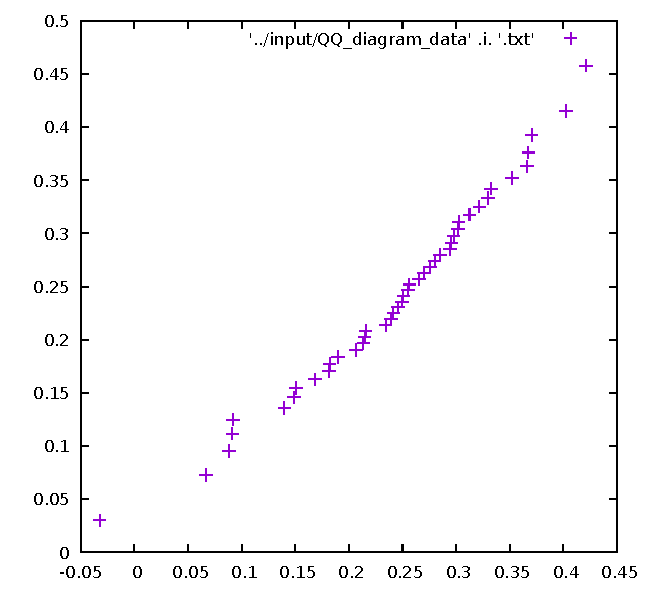
\includegraphics[width=0.3\textwidth]{../PCA/gnuplot/results_qq_diagrams/QQ_diagram4.pdf}}
  \qquad
  \subfloat[Länge der Hand]{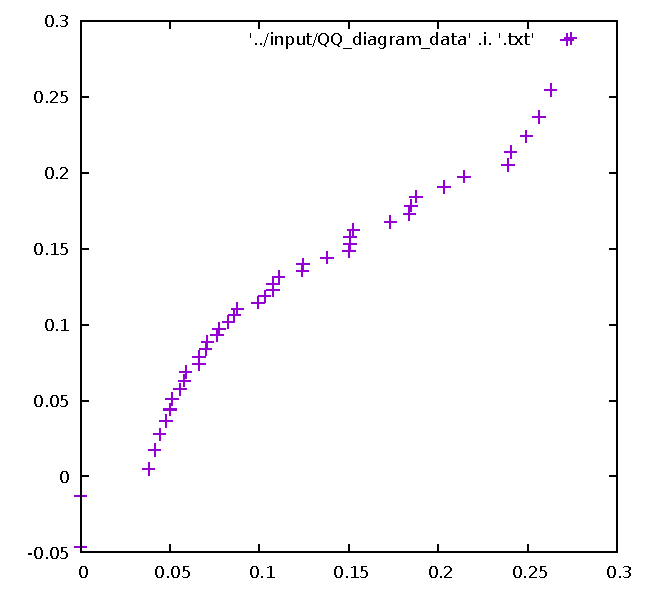
\includegraphics[width=0.3\textwidth]{../PCA/gnuplot/results_qq_diagrams/QQ_diagram24.pdf}}
  \qquad
  \subfloat[Länge des Oberschenkels]{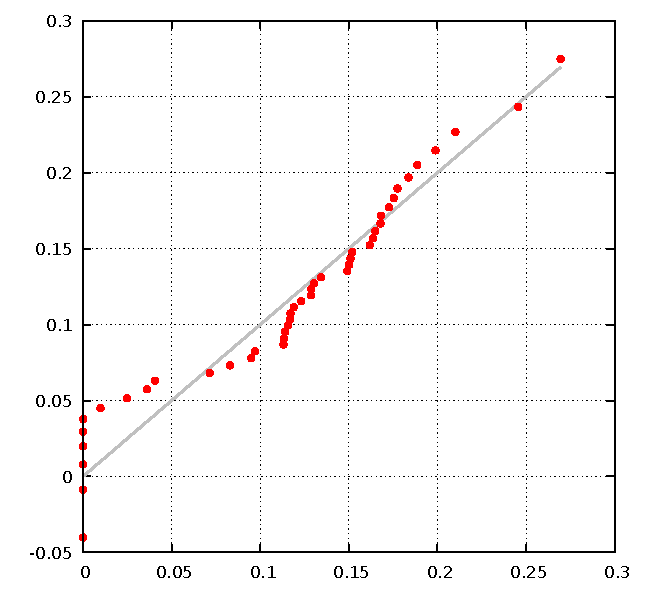
\includegraphics[width=0.3\textwidth]{../PCA/gnuplot/results_qq_diagrams/QQ_diagram25.pdf}}
  
  \caption{Beispielhaft ausgewählte Quantil-Quantil-Diagramme von drei Eingabedimensionen. (a) weicht nicht stark von der Normalverteilung ab, (b) und (c) hingegen schon mehr, sind aber trotzdem noch akzeptabel verteilt.}
  \label{qqdiagram_examples}
 \end{figure}
 
 \begin{figure}
  \subfloat[Gewicht linear]{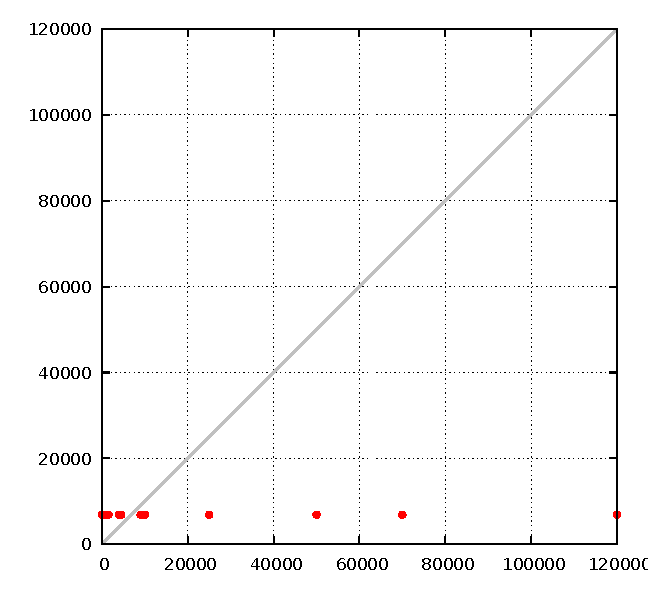
\includegraphics[width=0.3\textwidth]{../PCA/gnuplot/results_qq_diagrams/QQ_diagram_linear_weight.pdf}}
  \qquad
  \subfloat[Gewicht linear (Ausschnitt)]{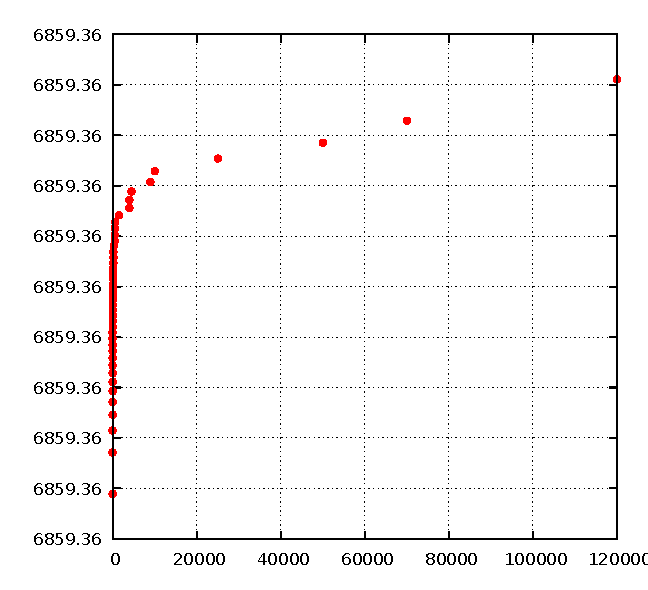
\includegraphics[width=0.3\textwidth]{../PCA/gnuplot/results_qq_diagrams/QQ_diagram_linear_weight_without_diagonal.pdf}}
  \qquad
  \subfloat[Gewicht logarithmisch]{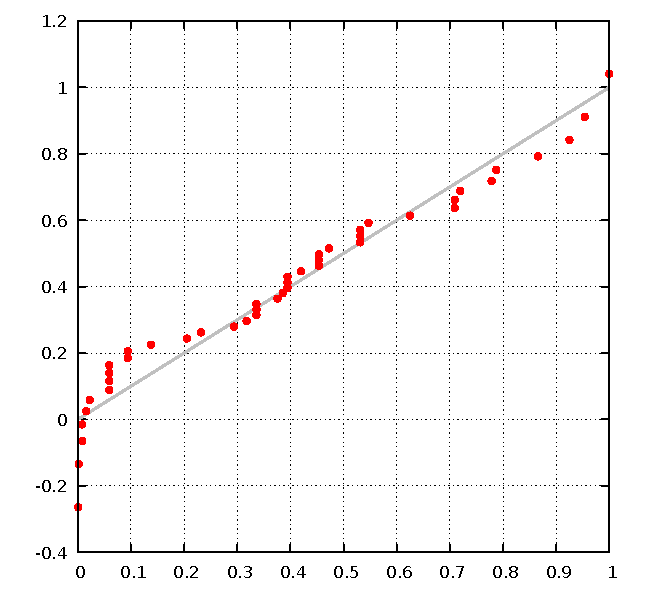
\includegraphics[width=0.3\textwidth]{../PCA/gnuplot/results_qq_diagrams/QQ_diagram28.pdf}}
  
  \caption{ Quantil-Quantil-Diagramme des Gewichts, einmal linear (a,b) und einmal mit logarithmischer Skala (b)}
  \label{qqdiagrams_weight}
 \end{figure}
 
 % Gewichtung der Daten
 Generell bewirkt die Skalierung einer Dimension eine Gewichtung, denn durch eine Skalierung ändert sich die (Ko-)Varianz und somit auch die Kovarianzmatrix. Seien beispielsweise $s,t \in \mathbb{R}$, dann bewirkt eine Skalierung mit $s$ in Dimension $x$ und eine Skalierung mit $t$ in Dimension $y$ eine Skalierung von $s \cdot t$ der Kovarianz Cov$(x,y)$ von $x$ mit $y$, da $\mathrm{Cov}(sx, ty) = (sx - s\mu_x) (ty - t\mu_y) = st \cdot \mathrm{Cov}(x,y)$, mit Erwartungswert $\mu_i$ in \mbox{Dimension $i$}.
 
 Wie genau wurden nun die einzelnen Merkmale nur skaliert?
 
 % Bildkoordinaten + -längen
 Zunächst wurden alle Merkmale auf das Intervall $[0, 1]$ skaliert, damit alle den gleichen Einfluss haben.
 Bei Koordinaten oder Längen im Bild bedeutet das, dass sie durch $1000$ geteilt werden, da sie in Pixeln dargestellt werden und das Bild eine Größe von $1000 \times 1000$ Pixeln hat. Bei Längen wären dabei theoretisch auch Werte größer $1000$px möglich. Solche Längen wären aber unrealistisch und werden deshalb ignoriert.\\
 Koordinaten und Längen im Bild sind diejenigen Merkmale, die hier am interessantesten sind. Deshalb sollten sie den größten Einfluss auf das Ergebnis der PCA haben. Alle anderen Merkmale werden deshalb kleiner skaliert.
 
 % Merkmale nach angenommenem Maximum skalieren?
 Man könnte statt einer Skalierung mit $0.001$ auch für jedes einzelne Merkmal den maximal und minimal angenommenen Wert ermitteln und sie dann so skalieren, dass sie Intervalle gleicher Länge abdecken. Das würde ausgleichen, dass \zb kleine Längen eine kleinere Varianz und damit auch einen kleineren Einfluss haben.
 Es wurde aber die oben beschriebene Variante verwendet, da es natürlich wirkt, dass kleine Merkmale im Bild auch weniger wichtig sind. Falls es in Zukunft Gründe für eine andere Gewichtung gäbe, ließe sich das aber leicht anpassen.
 
 % kleinskalieren von Flügeln, Beinen und Gewicht
 Die diskreten Merkmale \emph{Flügel} und \emph{Beine mit Bodenkontakt} und das logarithmische \emph{Gewicht} wurden zunächst ebenfalls auf das Intervall $[0, 1]$ skaliert. Das bedeutet für das angepasste Gewicht $\bar{w} = \frac{\mathrm{log}(w+1)}{\mathrm{log}(\mathrm{max}+1)}$. Das schwerste Wirbeltier ist der Blauwal mit 120 Tonnen (siehe Abschnitt \ref{bigAndSmall}). Deshalb ist hier max $= 120.000$kg.\\
 Danach wurden die Werte noch einmal durch $100$ geteilt, um ihren Einfluss zu verringern. Das Ziel war, dass diese Merkmale nicht als große Einträge in den größten Eigenvektoren (den "`principal components"') auftauchen. Ohne diese Skalierung sind diese Merkmale recht dominant. Mit der Skalierung hingegen sind sie in den größten Eigenvektoren unter den kleinsten Werten zu finden.
 
 % Projektion auf Eigenvektoren
 Interessant ist die Projektion der Eingabedaten auf die größten beiden  Eigenvektoren. In Abbildung \ref{projections_scales} ist gut zu vergleichen was die Effekte der Skalierung der Eingabedaten sind. Ganz links sind die Ergebnisse zusehen, die entstehen, wenn alle Merkmale nur auf das Intervall $[0, 1]$ skaliert werden. In der Mitte geht das Gewicht nicht mehr linear, sondern logarithmisch ein und ganz rechts sind \emph{Flügel}, \emph{Anzahl Beine} und \emph{Gewicht} zusätzlich klein skaliert. Gut zu sehen ist, wie sich die Clusterbildung durch die Anpassungen verringert.
 
 % Projektion unterschiedlich gelabelt
 In Abbildung \ref{projections_tags} ist noch einmal jeweils die Projektion der skalierten Daten auf die ersten beiden Eigenvektoren zu sehen. Diesmal sind die Daten anhand der verschiedenen diskret erhobenen Merkmale markiert. Es ist \zb schön zu sehen, dass alle Tiere mit Flügeln auch Vögel sind und dass fast alle Tiere, die zwei Beine haben, Vögel sind. Vier Tiere haben zwei Beine, sind aber keine Vögel: die Ohrenrobbe, der Seehund, der Tyrannosaurus Rex und das Känguru.

 \begin{figure}
  \subfloat[gleiche Skalierung aller Dimensionen]{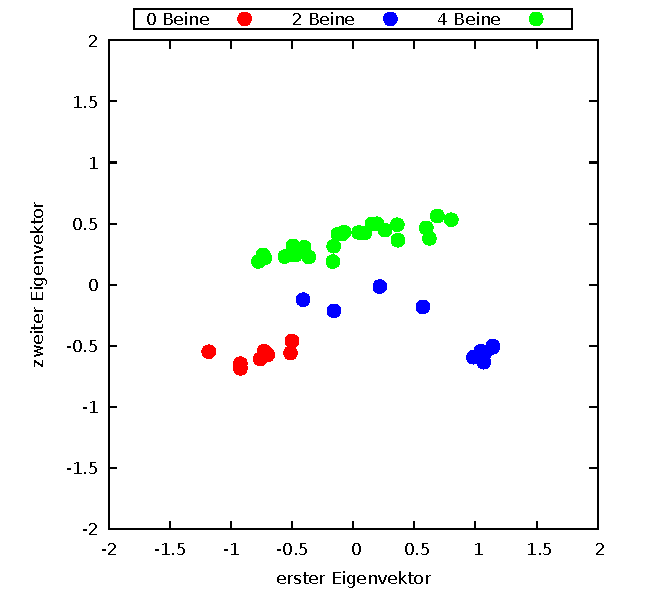
\includegraphics[width=0.3\textwidth]{../PCA/gnuplot/results_with_leg_tag/projection_eigenvectors12.pdf}}
  \qquad
  \subfloat[logarithmisches Gewicht]{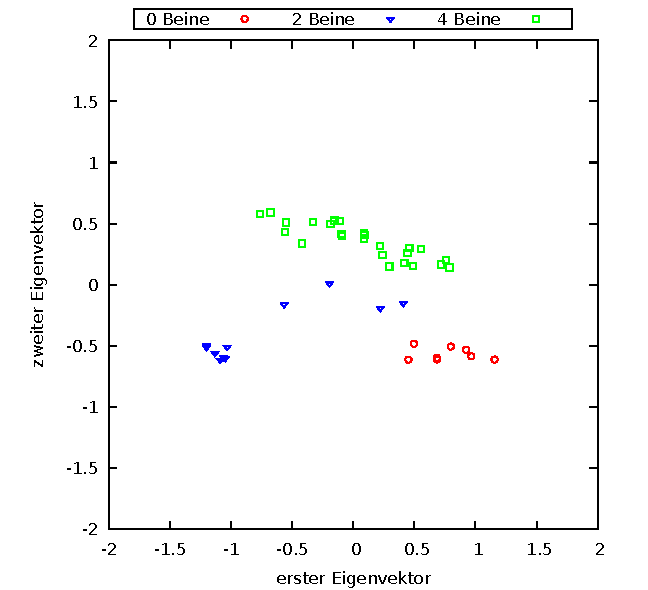
\includegraphics[width=0.3\textwidth]{../PCA/gnuplot_log_weight/results_with_leg_tag/projection_eigenvectors12.pdf}}
  \qquad
  \subfloat[skalierte "`Zusatzmerkmale"']{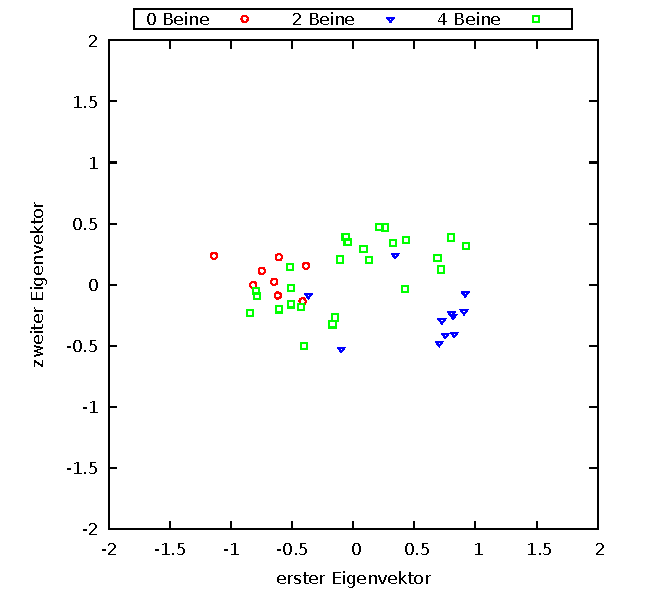
\includegraphics[width=0.3\textwidth]{../PCA/gnuplot_log_weight_with_downscaled_wings_legs_and_weight/results_with_leg_tag/projection_eigenvectors12.pdf}}
  
  \caption{Dargestellt sind hier jeweils die Projektionen der Eingabedaten auf die ersten beiden Eigenvektoren. Für jede Version wurden die Eingabedaten unterschiedlich vorverarbeitet. (a) Skalierung aller erhobenen Daten auf das Intervall $[0, 1]$, (b) zusätzlich Verwendung von logarithmischem Gewicht, statt linearem, (c) zusätzliche Skalierung der Merkmale \emph{Flügel}, \emph{Anzahl Beine} und \emph{Gewicht} mit $0,01$. In \mbox{Version (b)} wurde der erste Eigenvektor durch die PCA umgedreht, weshalb das Cluster der Zweibeiner auf der linken, statt der rechten Seite zu sehen ist.}
  \label{projections_scales}
 \end{figure}
 
 \begin{figure}
  \subfloat[Flügel]{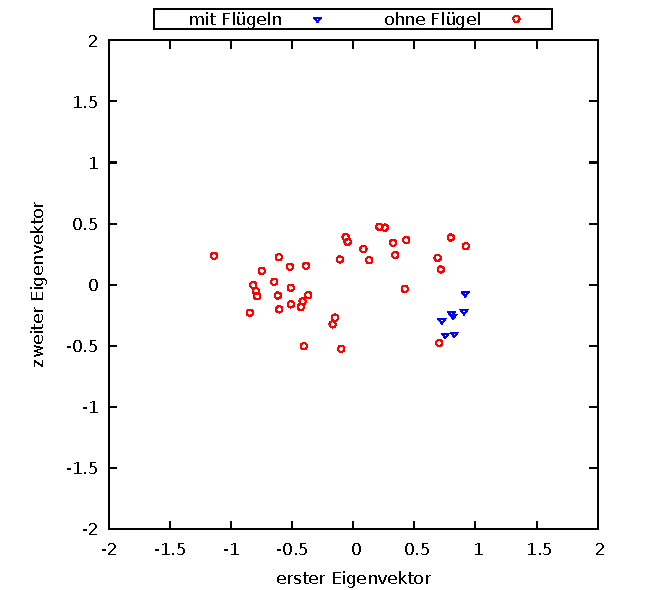
\includegraphics[width=0.3\textwidth]{../PCA/gnuplot_log_weight_with_downscaled_wings_legs_and_weight/results_with_wing_tag/projection_eigenvectors12.pdf}}
  \qquad
  \subfloat[Anzahl Beine mit Bodenkontakt]{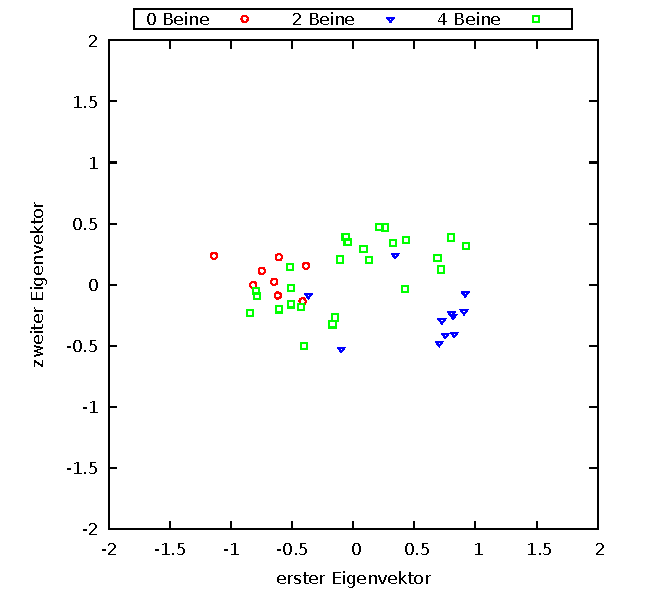
\includegraphics[width=0.3\textwidth]{../PCA/gnuplot_log_weight_with_downscaled_wings_legs_and_weight/results_with_leg_tag/projection_eigenvectors12.pdf}}
  \qquad
  \subfloat[Tierklasse]{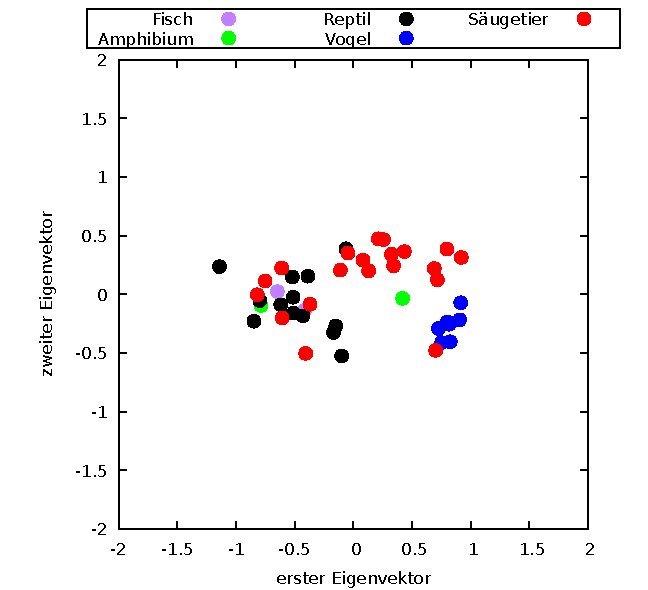
\includegraphics[width=0.3\textwidth]{../PCA/gnuplot_log_weight_with_downscaled_wings_legs_and_weight/results_with_animal_class_tag/projection_eigenvectors12.pdf}}
  
  \caption{Projektion der, wie in Abbildung \ref{projections_scales}c skalierten, Eingabedaten auf die Ebene, die durch den ersten und zweiten Eigenvektor aufgespannt wird. Markiert sind jeweils ob Flügel vorhanden sind (a), die Anzahl der Beine (b) und die \mbox{Tierklasse (c)}.}
  \label{projections_tags}
 \end{figure}
 
 
 % Ergebnis wieder normalverteilt
 Auch im Koordinatensystem der Eigenvektoren sollten die Daten wieder normalverteilt sein. Dies wurde ebenfalls mit Quantil-Quantil-Diagrammen untersucht. In Abbildung \ref{qqdiagram_projections} sind die Ergebnisse für die ersten drei Eigenvektoren zu sehen. Es gibt, wie bei den Eingabedaten, keine allzu großen Abweichungen.
 
 \begin{figure}
  \subfloat[erster Eigenvektor]{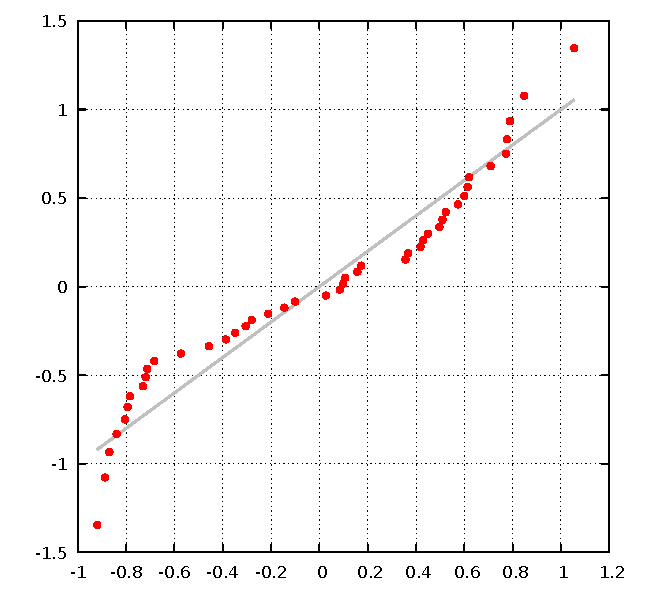
\includegraphics[width=0.3\textwidth]{../PCA/gnuplot_log_weight_with_downscaled_wings_legs_and_weight/results_qqdiagrams/QQ_diagram_projection0.pdf}}
  \qquad
  \subfloat[zweiter Eigenvektor]{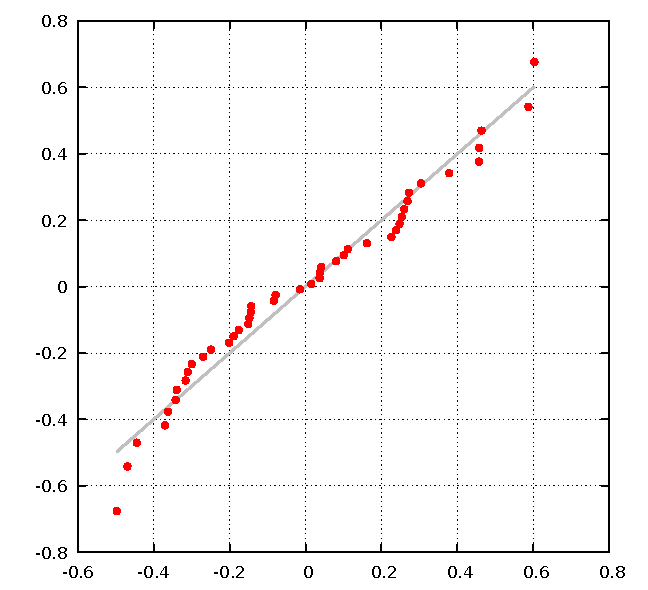
\includegraphics[width=0.3\textwidth]{../PCA/gnuplot_log_weight_with_downscaled_wings_legs_and_weight/results_qqdiagrams/QQ_diagram_projection1.pdf}}
  \qquad
  \subfloat[dritter Eigenvektor]{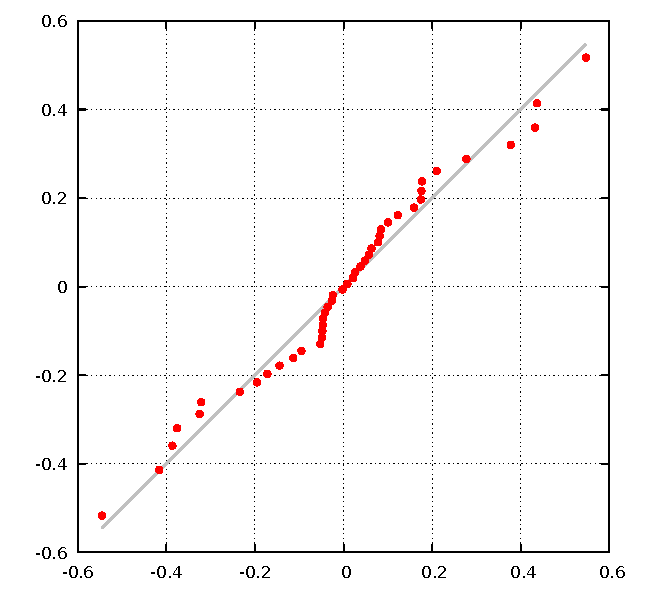
\includegraphics[width=0.3\textwidth]{../PCA/gnuplot_log_weight_with_downscaled_wings_legs_and_weight/results_qqdiagrams/QQ_diagram_projection2.pdf}}
  
  \caption{Quantil-Quantil-Diagramme der Eingabedaten projiziert auf die größten drei Eigenvektoren.}
  \label{qqdiagram_projections}
 \end{figure}
 
 
 % Mittelwert
 Der Mittelwert der skalierten Eingabedaten ist in Abbildung \ref{mean} visualisiert.
 Wie auch bei der Datenerhebung ist hier die Position der Wirbelsäule in einem $1000 \times 1000$ Pixel Bild gezeigt. Da von den Knochen der Vorder- und Hinterextremitäten nur die Längen erhoben wurden, sind ihre Positionen nicht realistisch. Die restlichen Daten sind nicht visualisiert, sondern nur in Textform angegeben.
 
 \begin{figure}
  \centering
  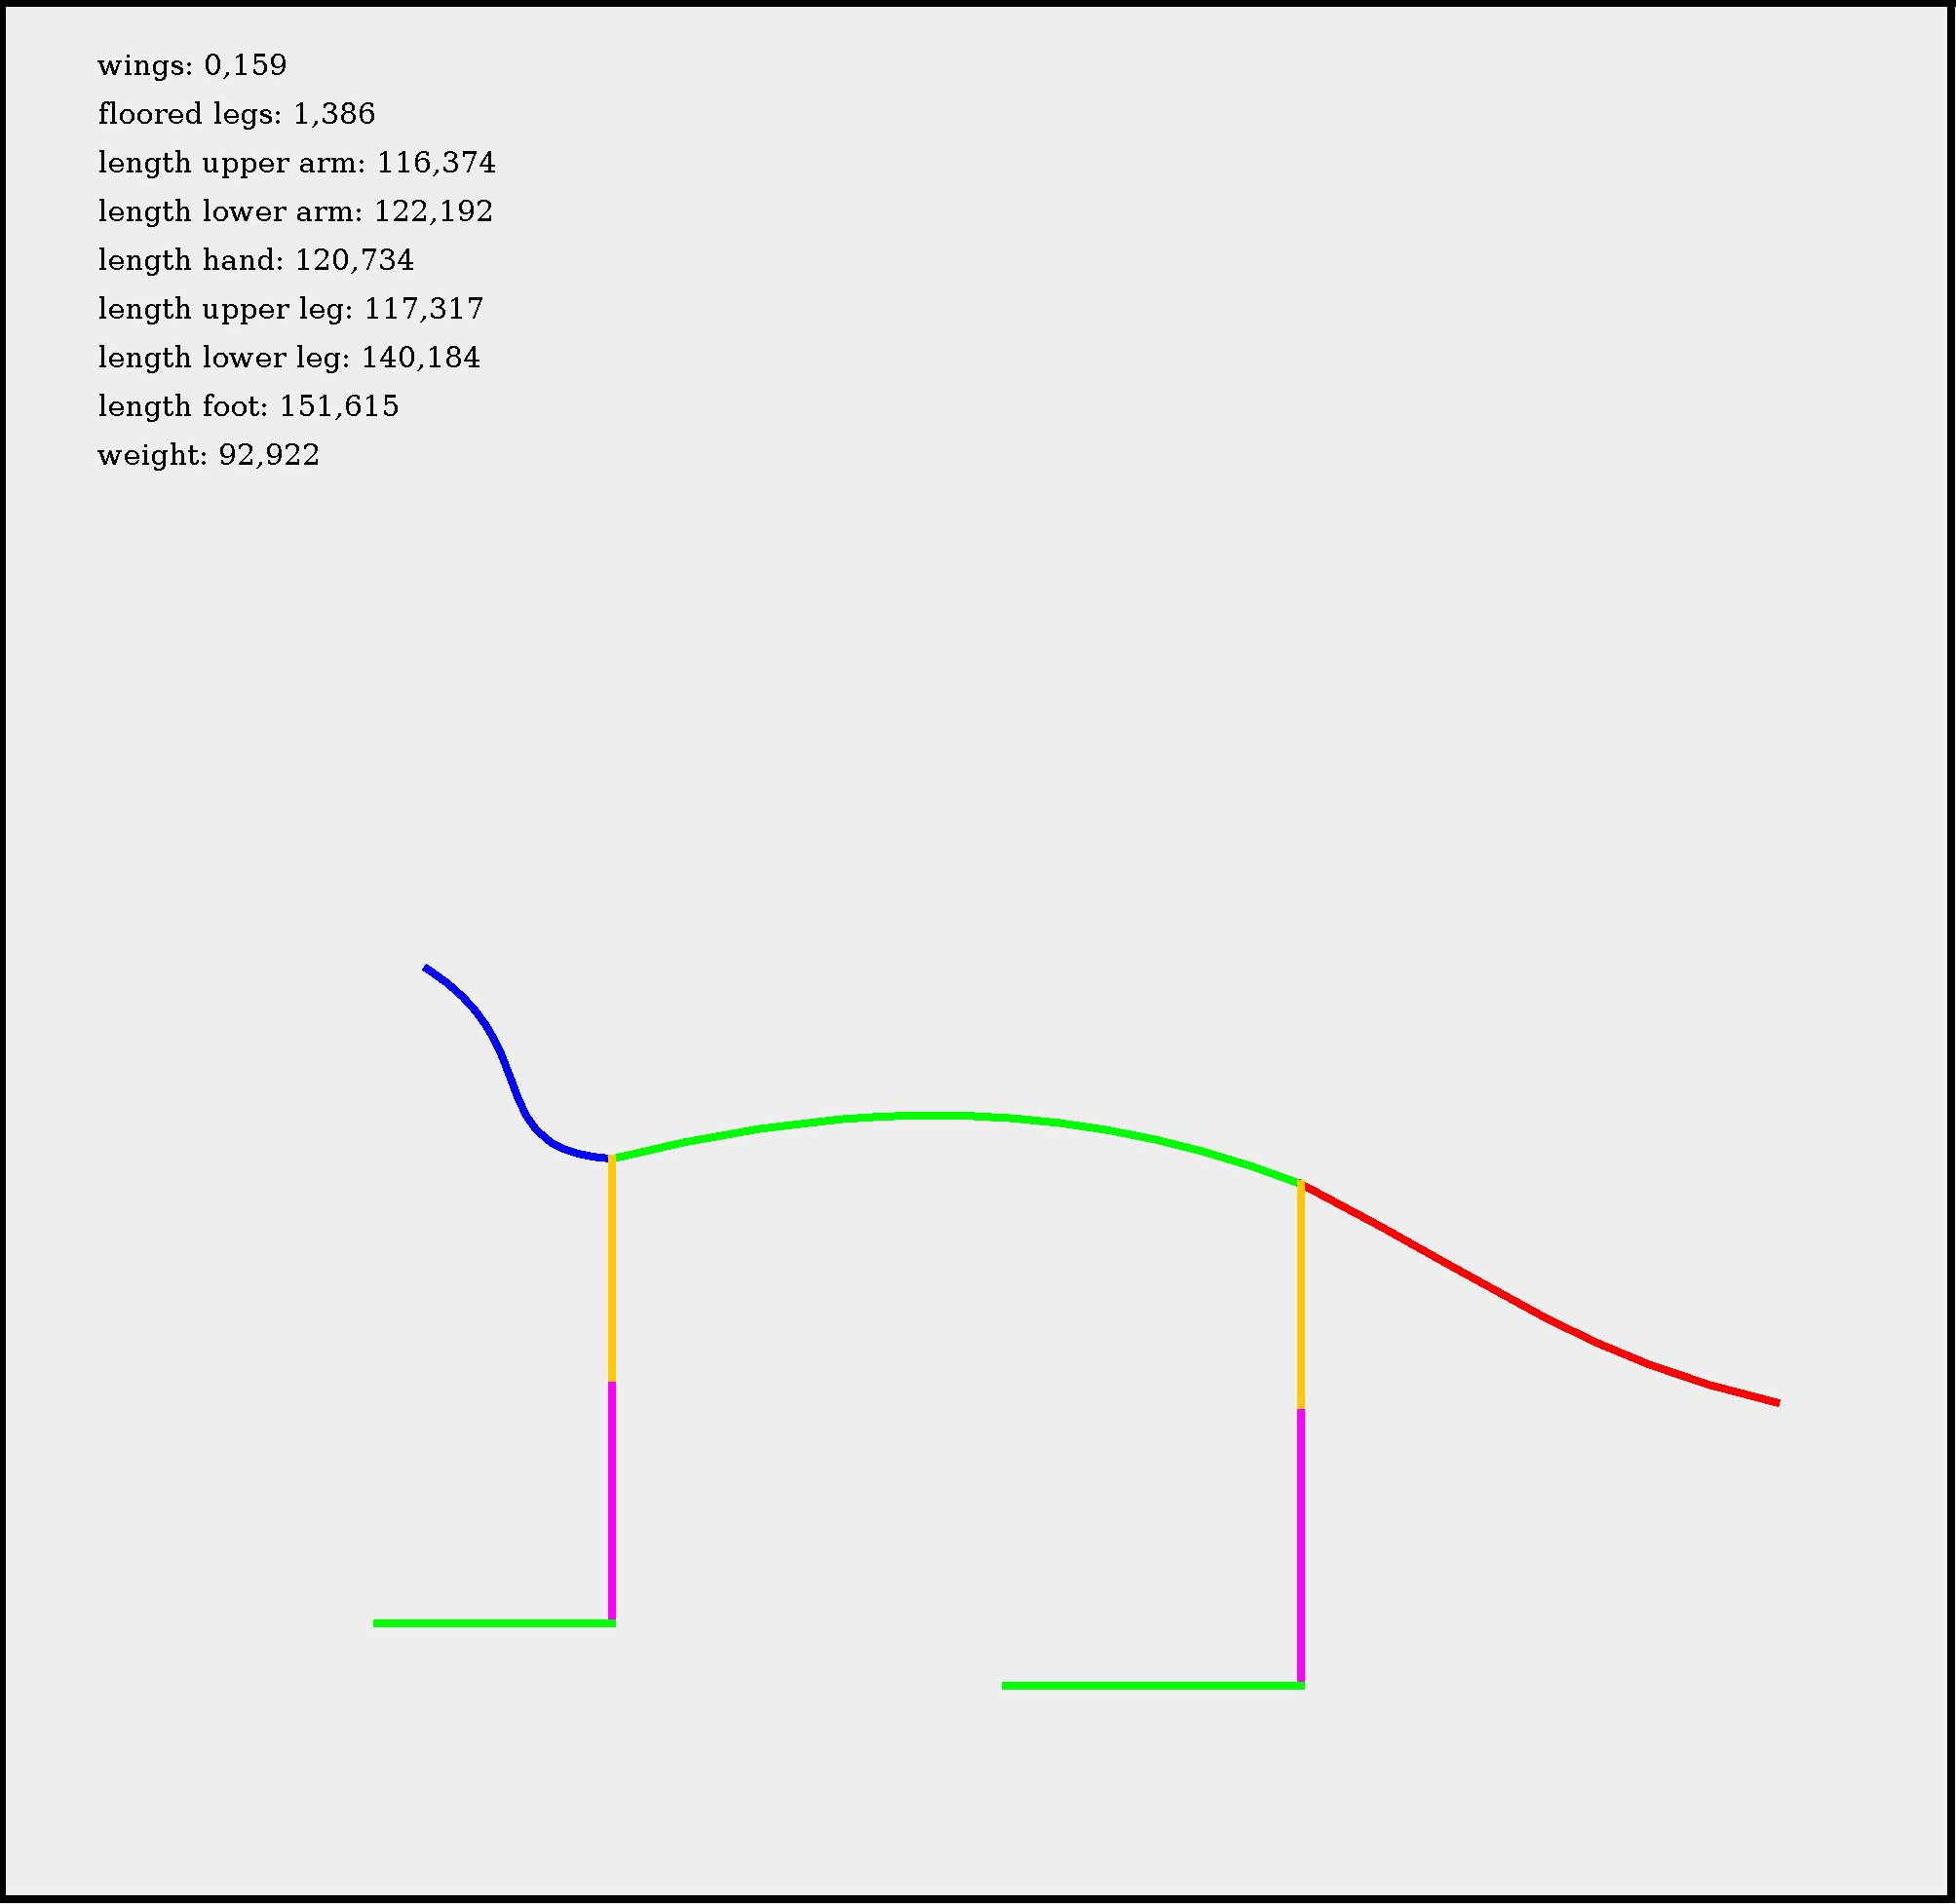
\includegraphics[width=0.5\textwidth]{../PCA/mean_log_weight_downscaled_wings_legs_and_weight(onlyBox,stroke4).jpg}
  \caption{Visualisierung des Mittelwerts der skalierten Eingabedaten. Die Werte, die nicht grafisch visualisiert sind, sind folgende: \emph{Flügel} $0,159$, \emph{Beine mit Bodenkontakt} $1,39$, \emph{Gewicht} $93$kg.}
  \label{mean}
 \end{figure}
 
 % min Abstand
 Den minimalen Abstand zum Mittelwert hat der Klippschliefer (siehe Abbildung \ref{klippschliefer_farbig}). Zusätzlich zum Bild wurde für den Klippschliefer folgende Daten erhoben:
 \emph{Tierklasse} Säugetier, \emph{Flügel} nein, \emph{Anzahl Beine mit Bodenkontakt} $4$, \emph{Gewicht} $4$kg.
 
 % max Abstand
 Den maximalen Abstand hat die Schlange. Die erhobenen Daten sind hier:
 \emph{Tierklasse} Reptil, \emph{Flügel} nein, \emph{Anzahl Beine mit Bodenkontakt} $0$, \emph{Gewicht} $50$kg.\\
 Die Schlange ist allerdings das einzige Tier zu dem es kein "`echtes"' Bild des Skeletts gibt. Das liegt daran, dass es keine seitlichen Abbildungen von ausgestreckten Schlangen gibt. Sie werden eigentlich immer gekrümmt dargestellt, da sonst das Bild sehr lang und schmal werden würde. Deshalb wurde für die Schlange nur eine horizontale Linie knapp über dem unteren Bildrand eingezeichnet, die den Rücken darstellen soll. Extremitäten und ersichtliche Punkte an denen der Rücken in Hals oder Schwanz übergeht gibt es bei Schlangen nicht.
 
 % zweitgrößter Abstand (da max Schlange)
 Der Punkt mit dem zweitgrößten Abstand zum Mittelwert ist das Känguru (siehe Abbildung \ref{kaenguru_farbig}). Zusätzlich zum Bild gibt es hier folgende Daten:
  \emph{Tierklasse} Säugetier, \emph{Flügel} nein, \emph{Anzahl Beine mit Bodenkontakt} $2$, \emph{Gewicht} $50$kg
  
 \begin{figure}
  \subfloat[Klippschliefer]{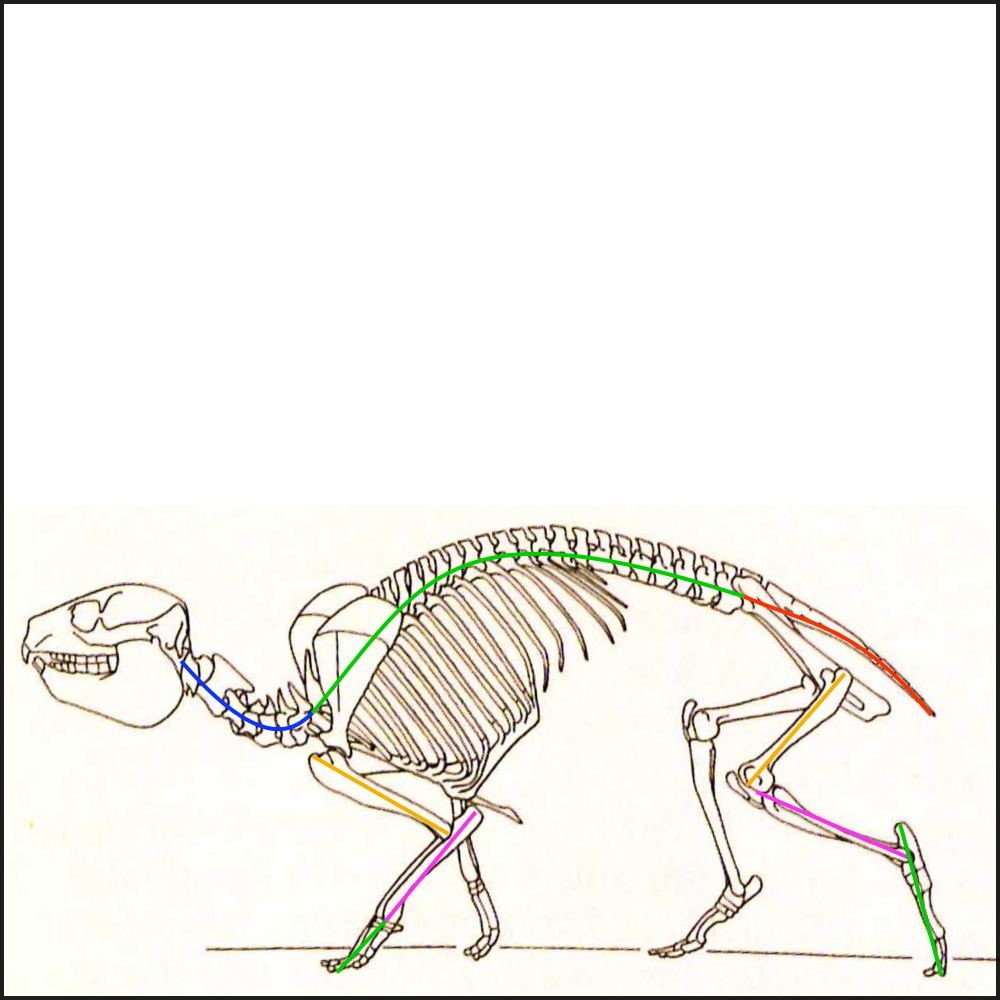
\includegraphics[width=0.5\textwidth]{../PCA/Skelettbilder/Klippschliefer_farbig.png} \label{klippschliefer_farbig}}
  \qquad
  \subfloat[Känguru]{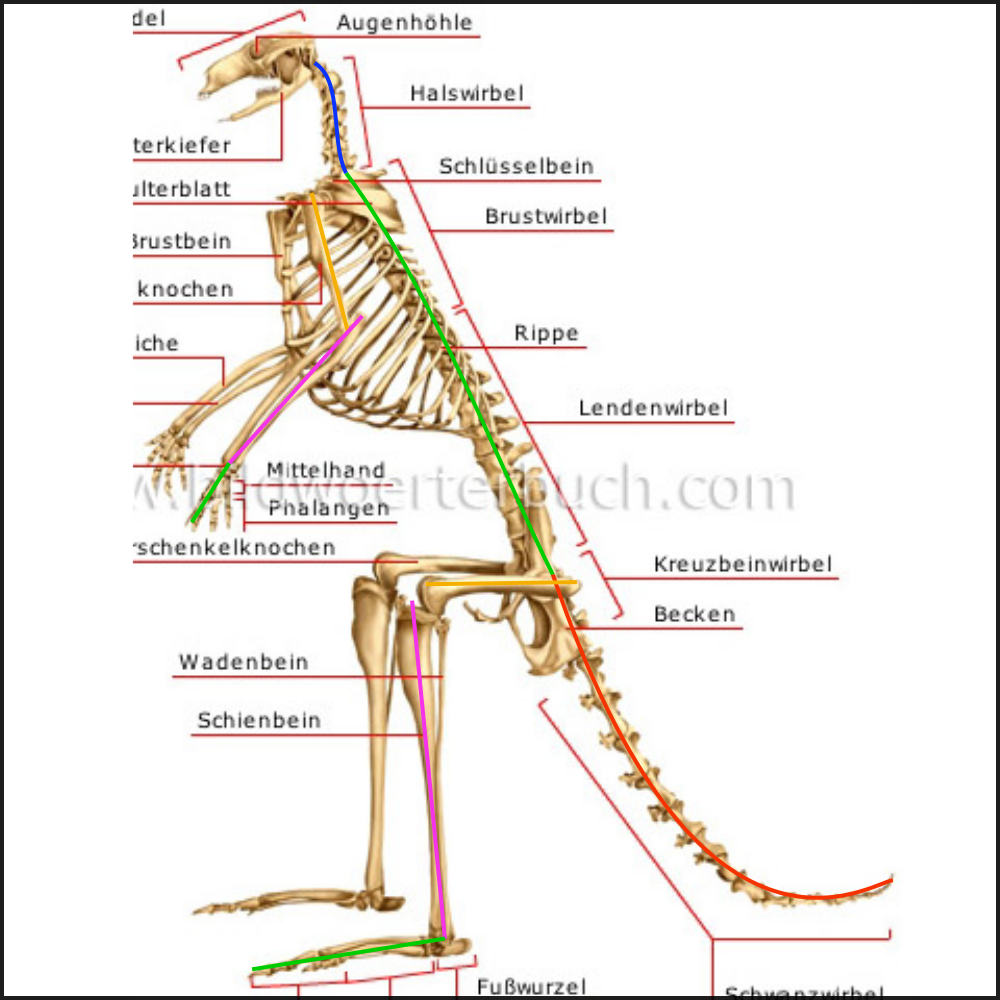
\includegraphics[width=0.5\textwidth]{../PCA/Skelettbilder/Kaenguru_farbig.png}\label{kaenguru_farbig}}
  
  \caption{Annotierte Bild des Skeletts eines Klippschliefers (a) und eines \mbox{Kängurus (b)}. Die Teile der Wirbelsäule und die Knochen der Extremitäten sind hier jeweils mit der gleichen Farbe markiert wie in der Visualisierung des Mittelwerts (Abbildung \ref{mean})}
 \end{figure}
 

 %-----------------------------------
 \section{Analyse der Ergebnisse}
 \label{section_pca_result_analysis}
 
 % Eigenvektoren und Rekonstruktionen
 Zu $29$ Eingabedimensionen gibt es auch $29$ Eigenvektoren mit Eigenwerten größer $0$. Der kleinste hat einen Eigenwert von $0,000001$. Von den Eigenwerten sind $6$ größer als $0,01$. Leider reichen diese $6$ Dimensionen noch nicht aus, um die Eingabedaten hinreichend anzunähern. Bei manchen Tieren funktioniert das zwar ganz gut (siehe Archaeopteryx, Abbildung \ref{archaeopteryx}), bei anderen aber eher schlechter (siehe Frosch, Abbildung \ref{frosch}).
 Die Daten konnten somit von der PCA nicht sehr gut komprimiert werden. Trotzdem sind die berechneten Eigenvektoren hilfreich um zufällige Punkte mit der Verteilung der Eingabebeispiele zu generieren (wie auch beschrieben in Abschnitt \ref{PCA}).
 
 \begin{figure}
  \subfloat[Rekonstruktion aus 6 Eigenvektoren]{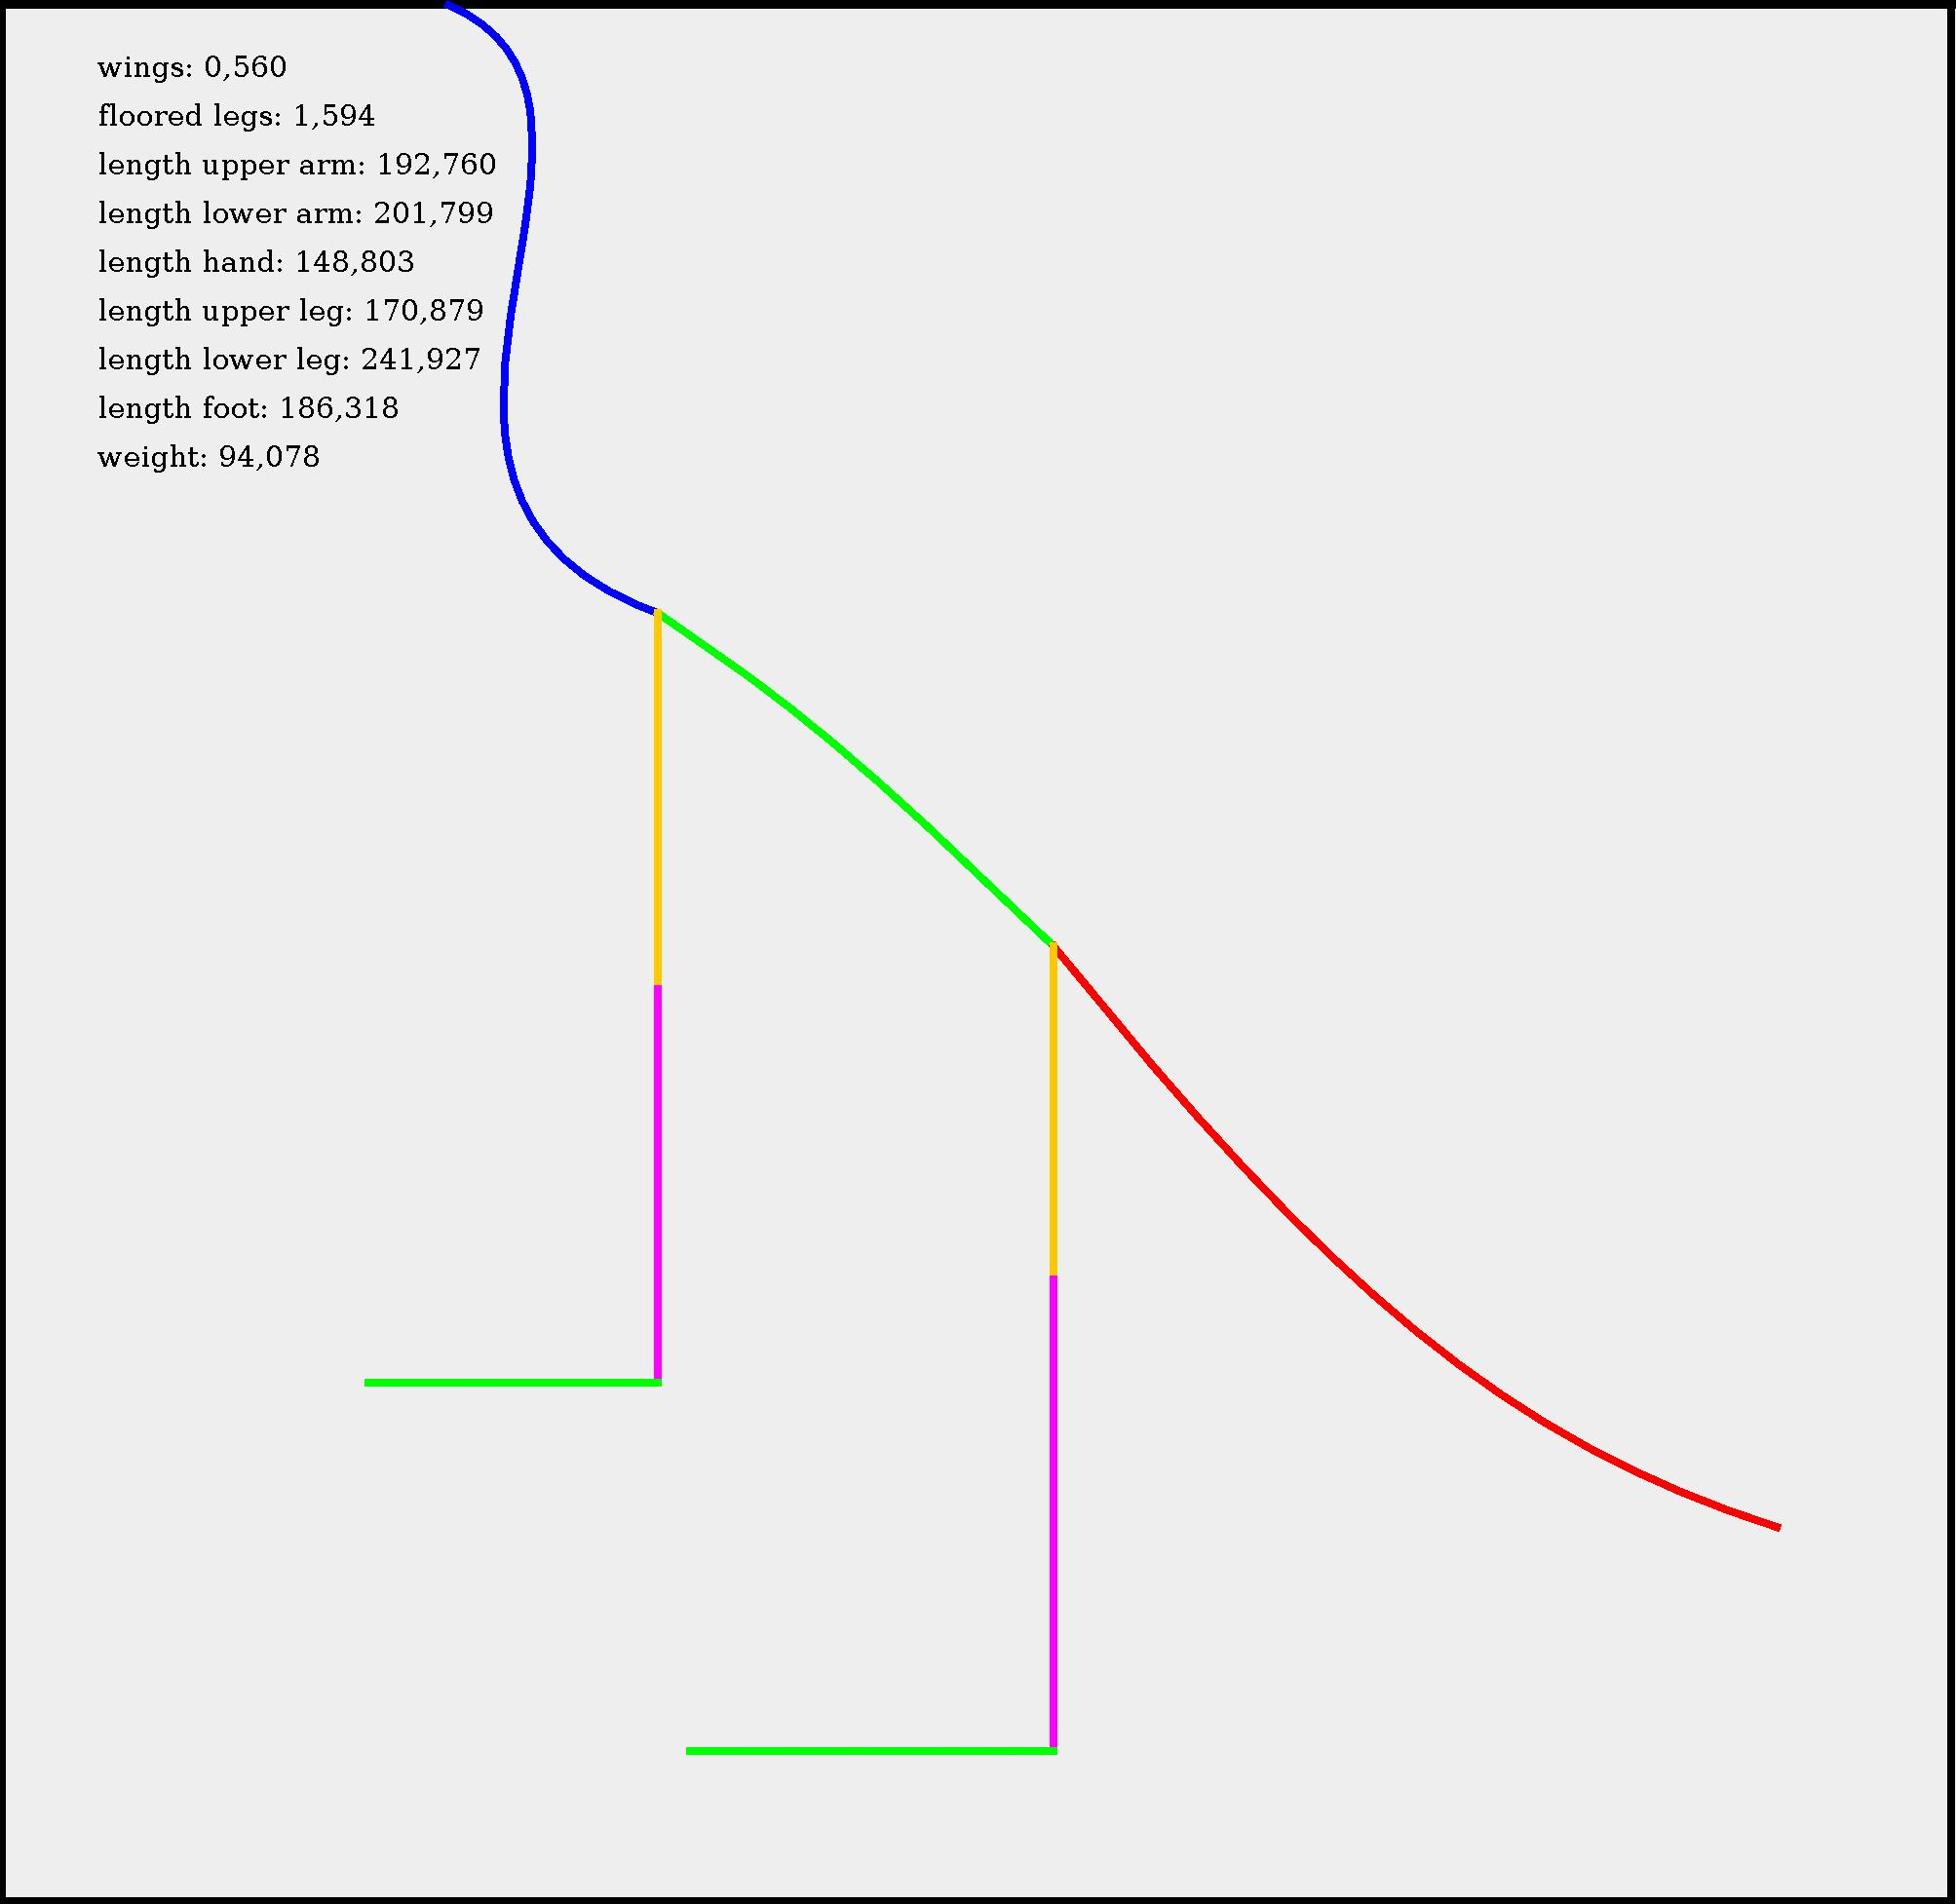
\includegraphics[width=0.5\textwidth]{../PCA/animal_reconstructions_log_weight_downscaled_wings_legs_and_weight/6EV/Archaeopteryx_Ausschnitt.jpg}}
  \qquad
  \subfloat[Eingabebild]{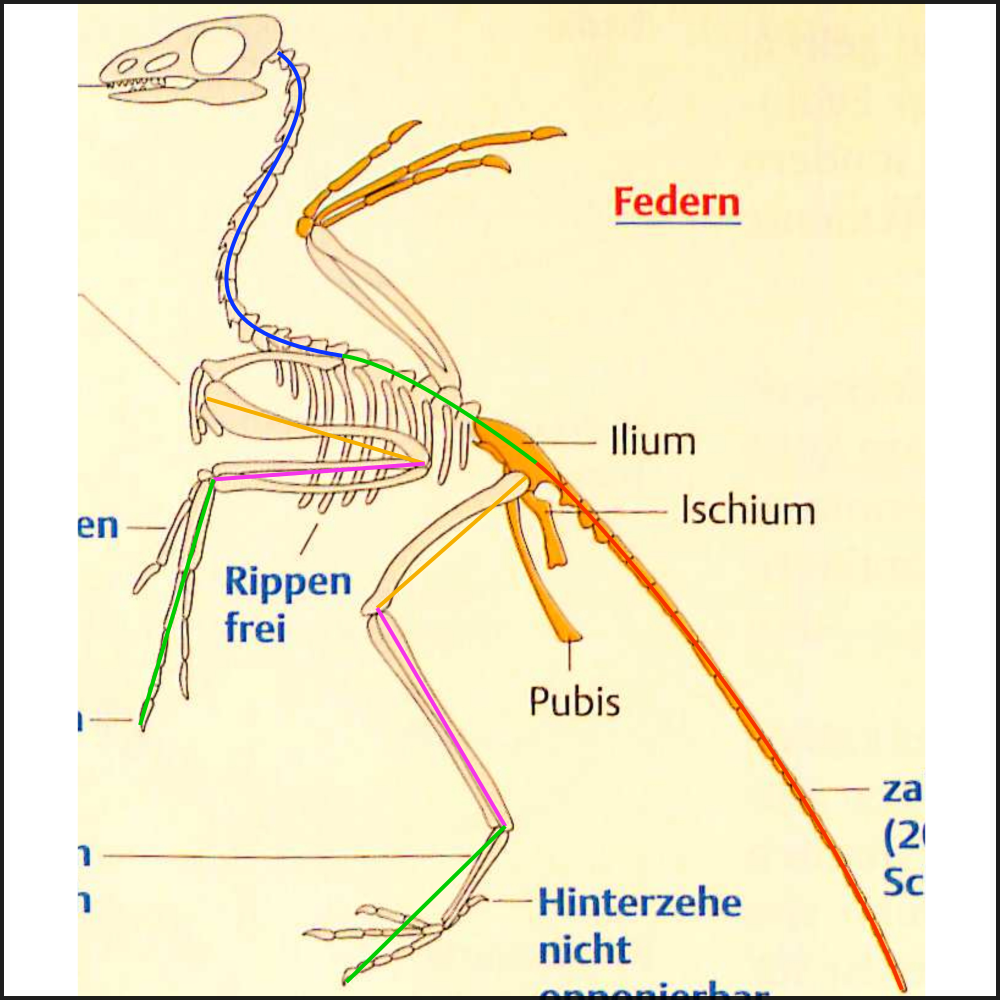
\includegraphics[width=0.5\textwidth]{../PCA/Skelettbilder/Archaeopteryx_farbig.png}}
  
  \caption{Archaeopteryx (a) Rekonstruktion aus den größten $6$ Eigenvektoren, nicht visualisierte Daten: \emph{Flügel} $0,56$, \emph{Beine mit Bodenkontakt} $1,594$, \emph{Gewicht} $94,1$kg\\ 
  (b) Eingabebild}
  \label{archaeopteryx}
 \end{figure}
 
\begin{figure}
  \subfloat[$6$ Eigenvektoren,
  \emph{Flügel} $0,4$, \emph{Beine mit Bodenkontakt} $1,27$, \emph{Gewicht} $90,2$kg]
  {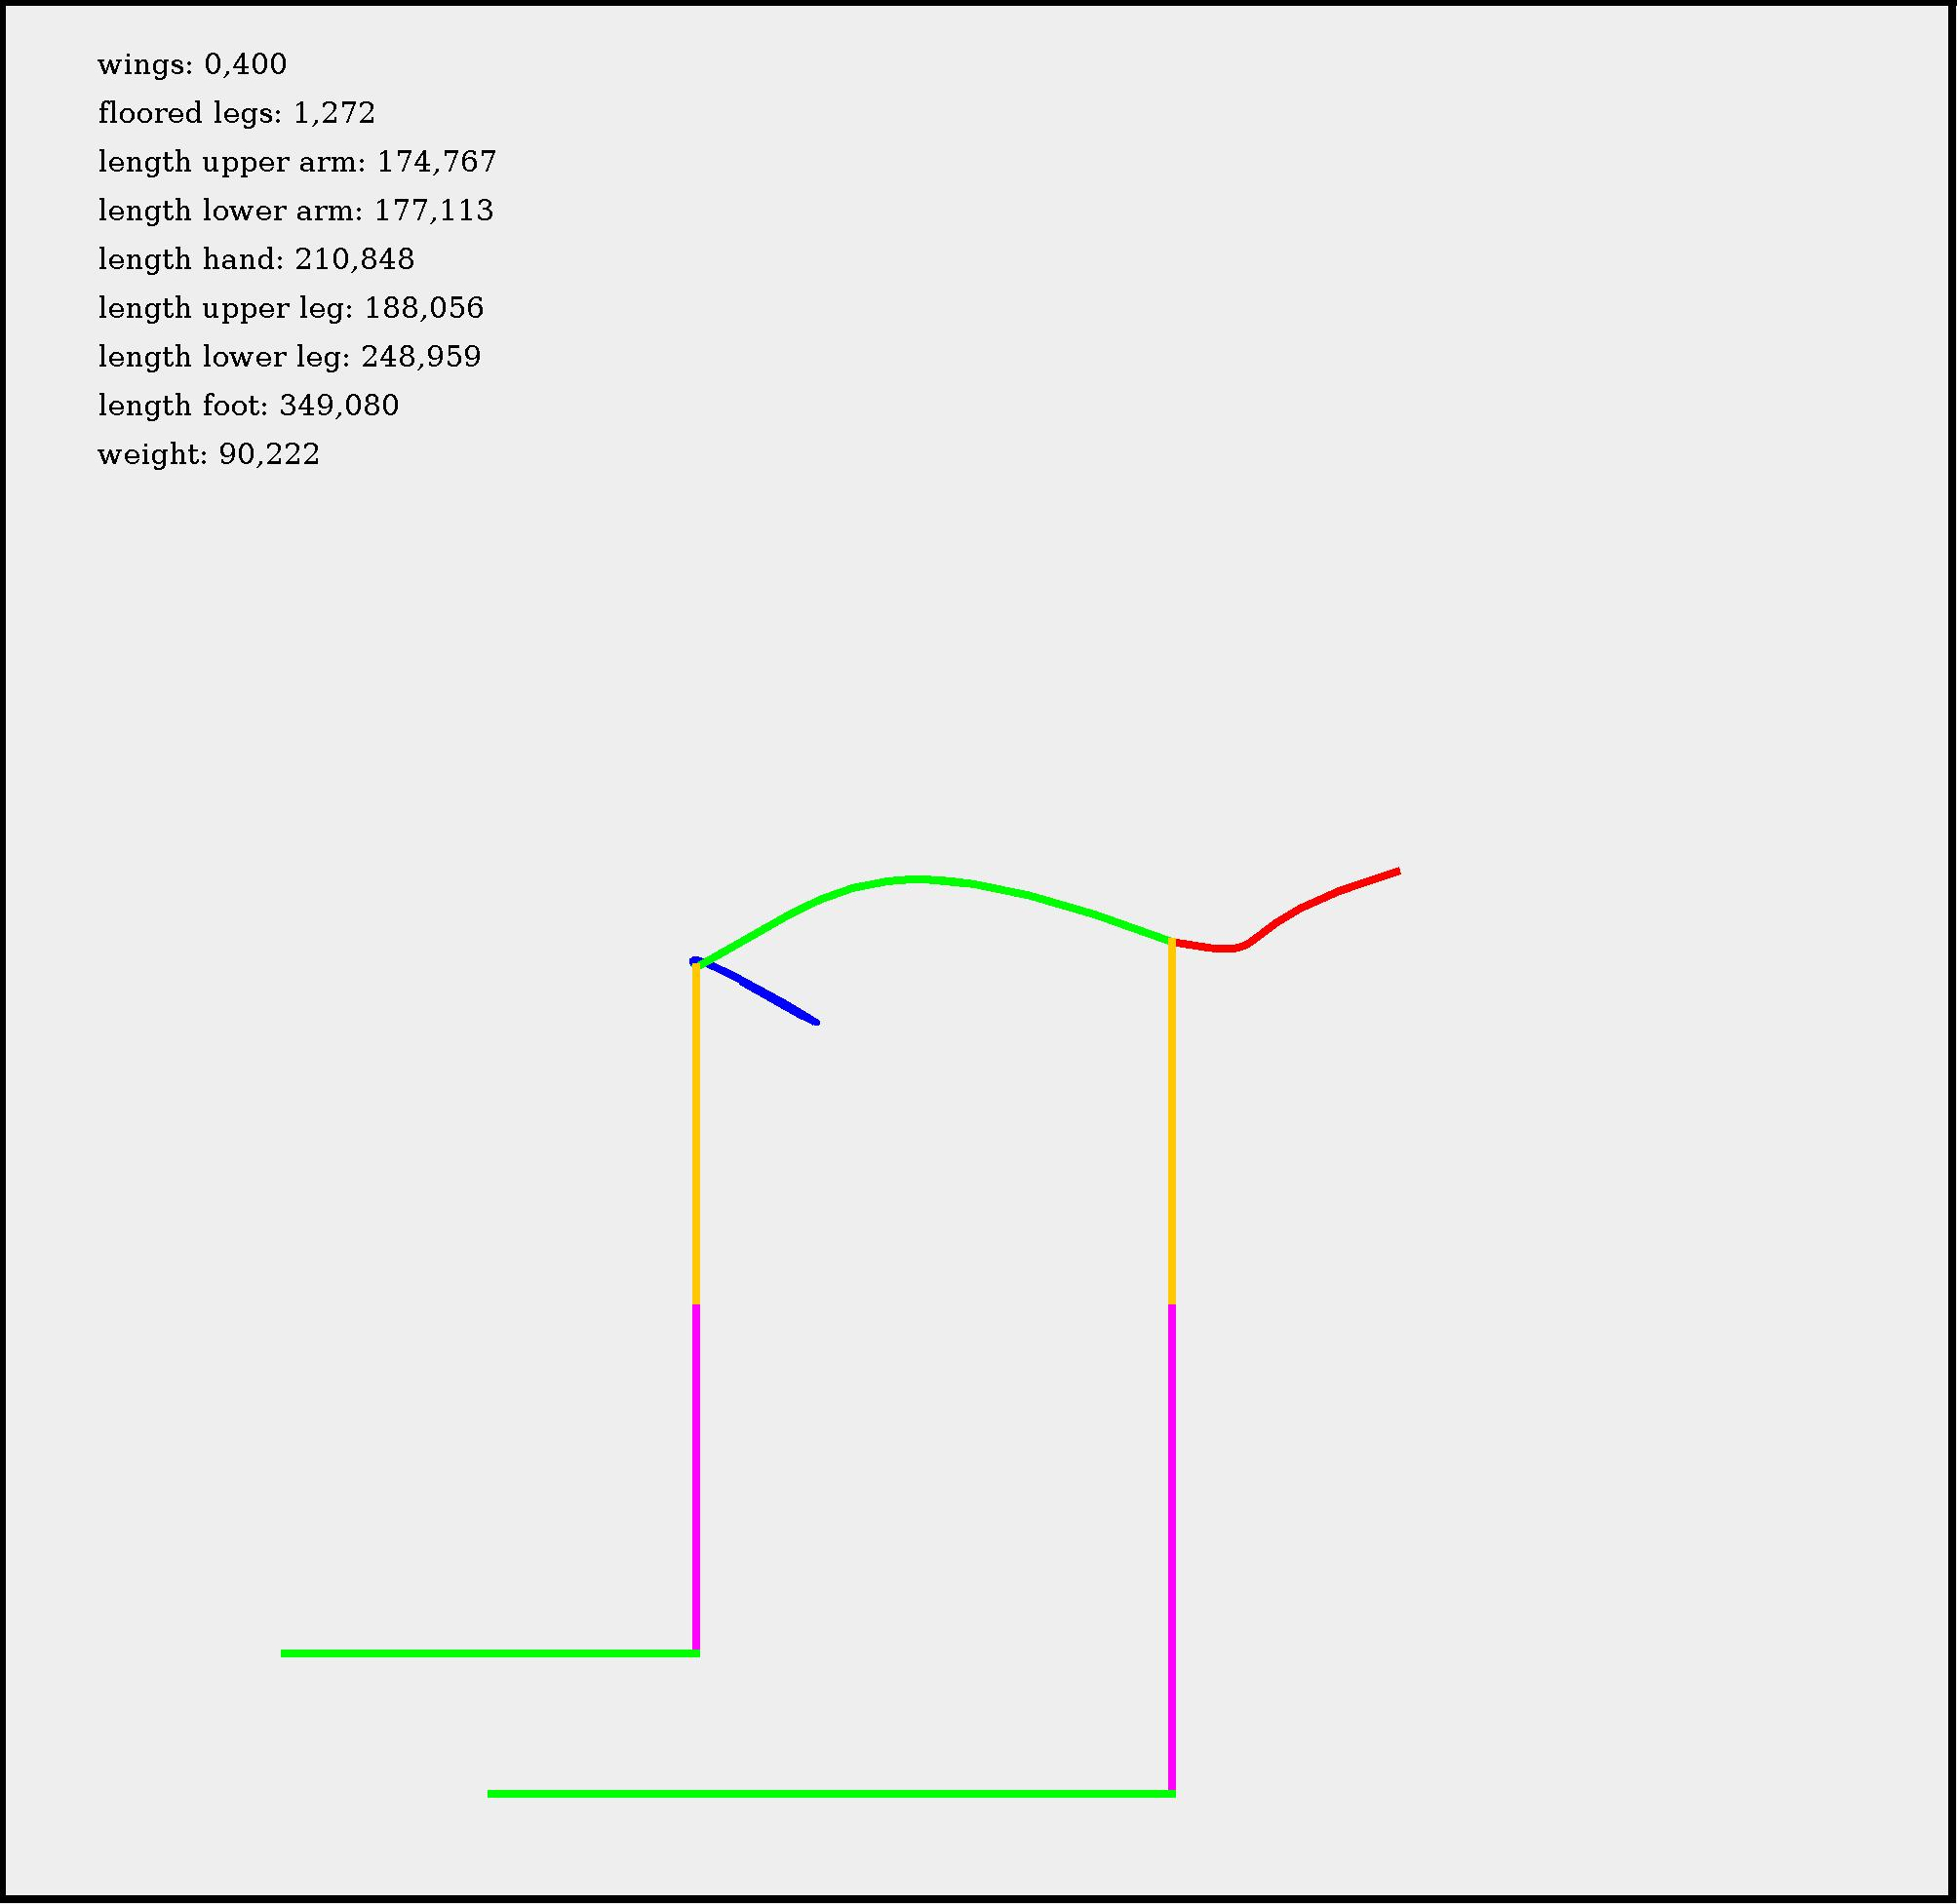
\includegraphics[width=0.5\textwidth]{../PCA/animal_reconstructions_log_weight_downscaled_wings_legs_and_weight/6EV/Frosch_Ausschnitt.jpg}}
  \qquad
  \subfloat[$10$ Eigenvektoren,
  \emph{Flügel} $0,151$, \emph{Beine mit Bodenkontakt} $1,28$, \emph{Gewicht} $88,7$kg]{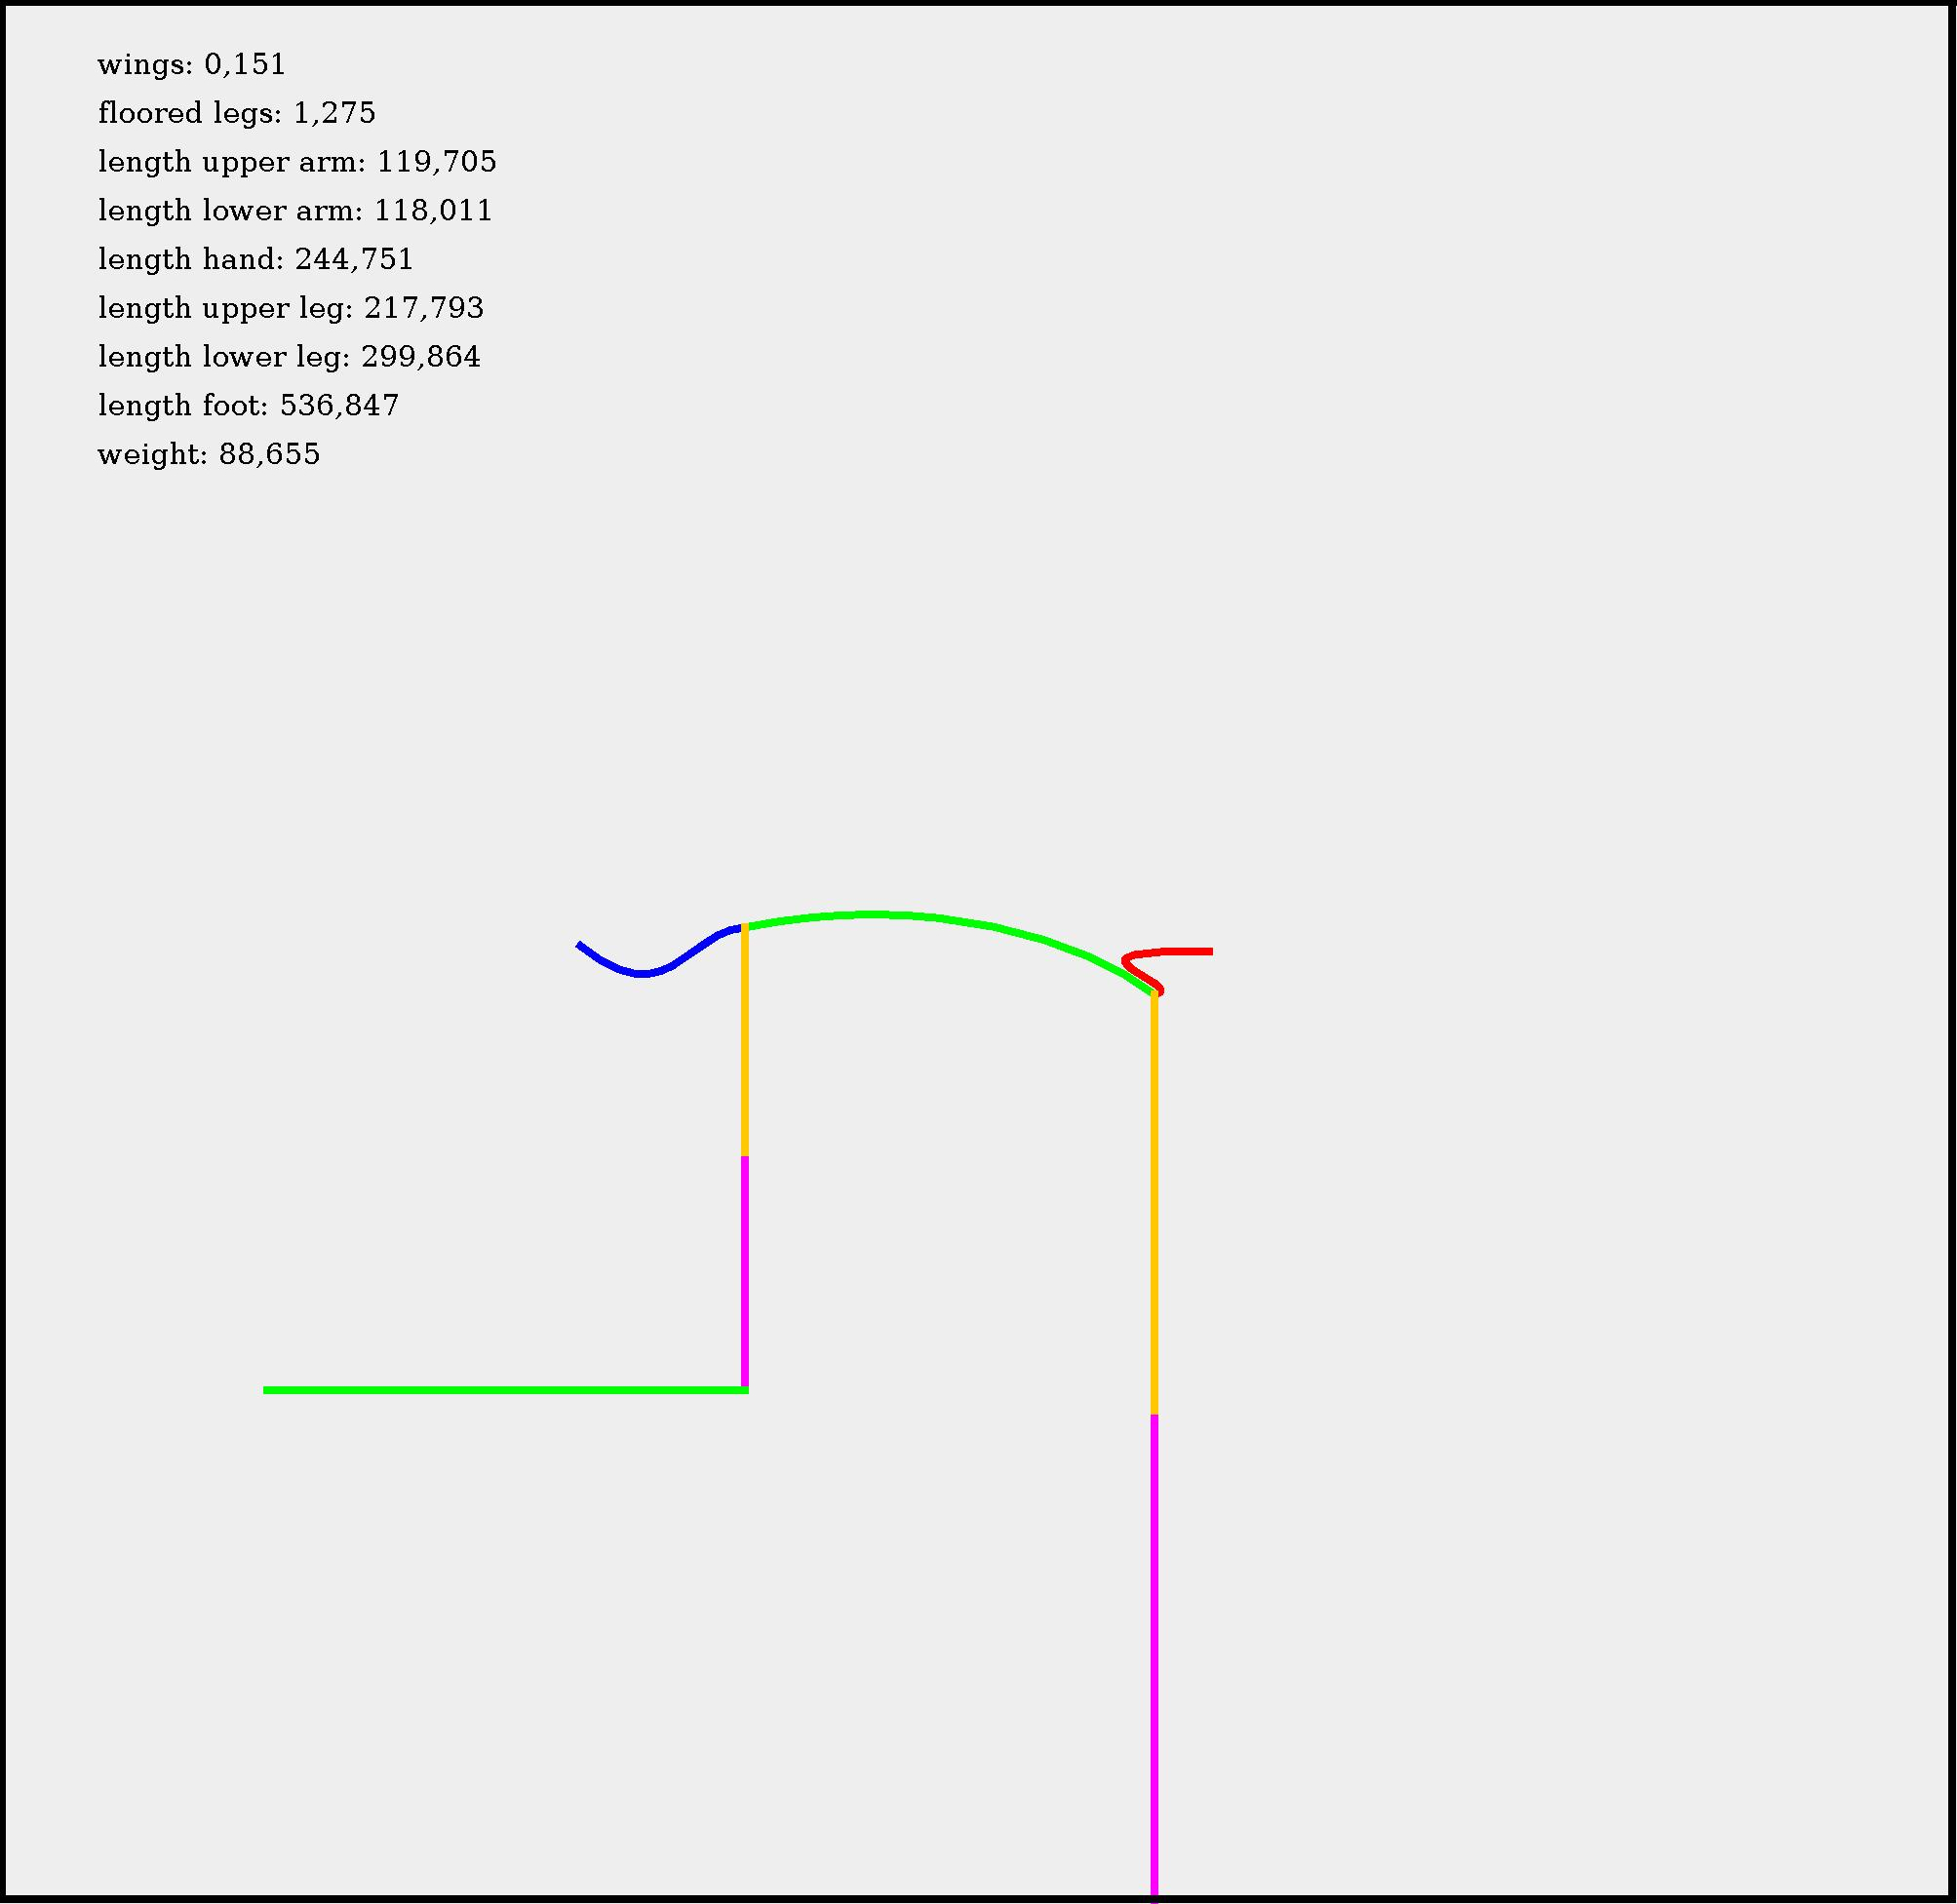
\includegraphics[width=0.5\textwidth]{../PCA/animal_reconstructions_log_weight_downscaled_wings_legs_and_weight/10EV/Frosch_Ausschnitt.jpg}}
  \\
  \subfloat[$20$ Eigenvektoren,
  \emph{Flügel} $0,217$, \emph{Beine mit Bodenkontakt} $1,7$, \emph{Gewicht} $89,2$kg]
  {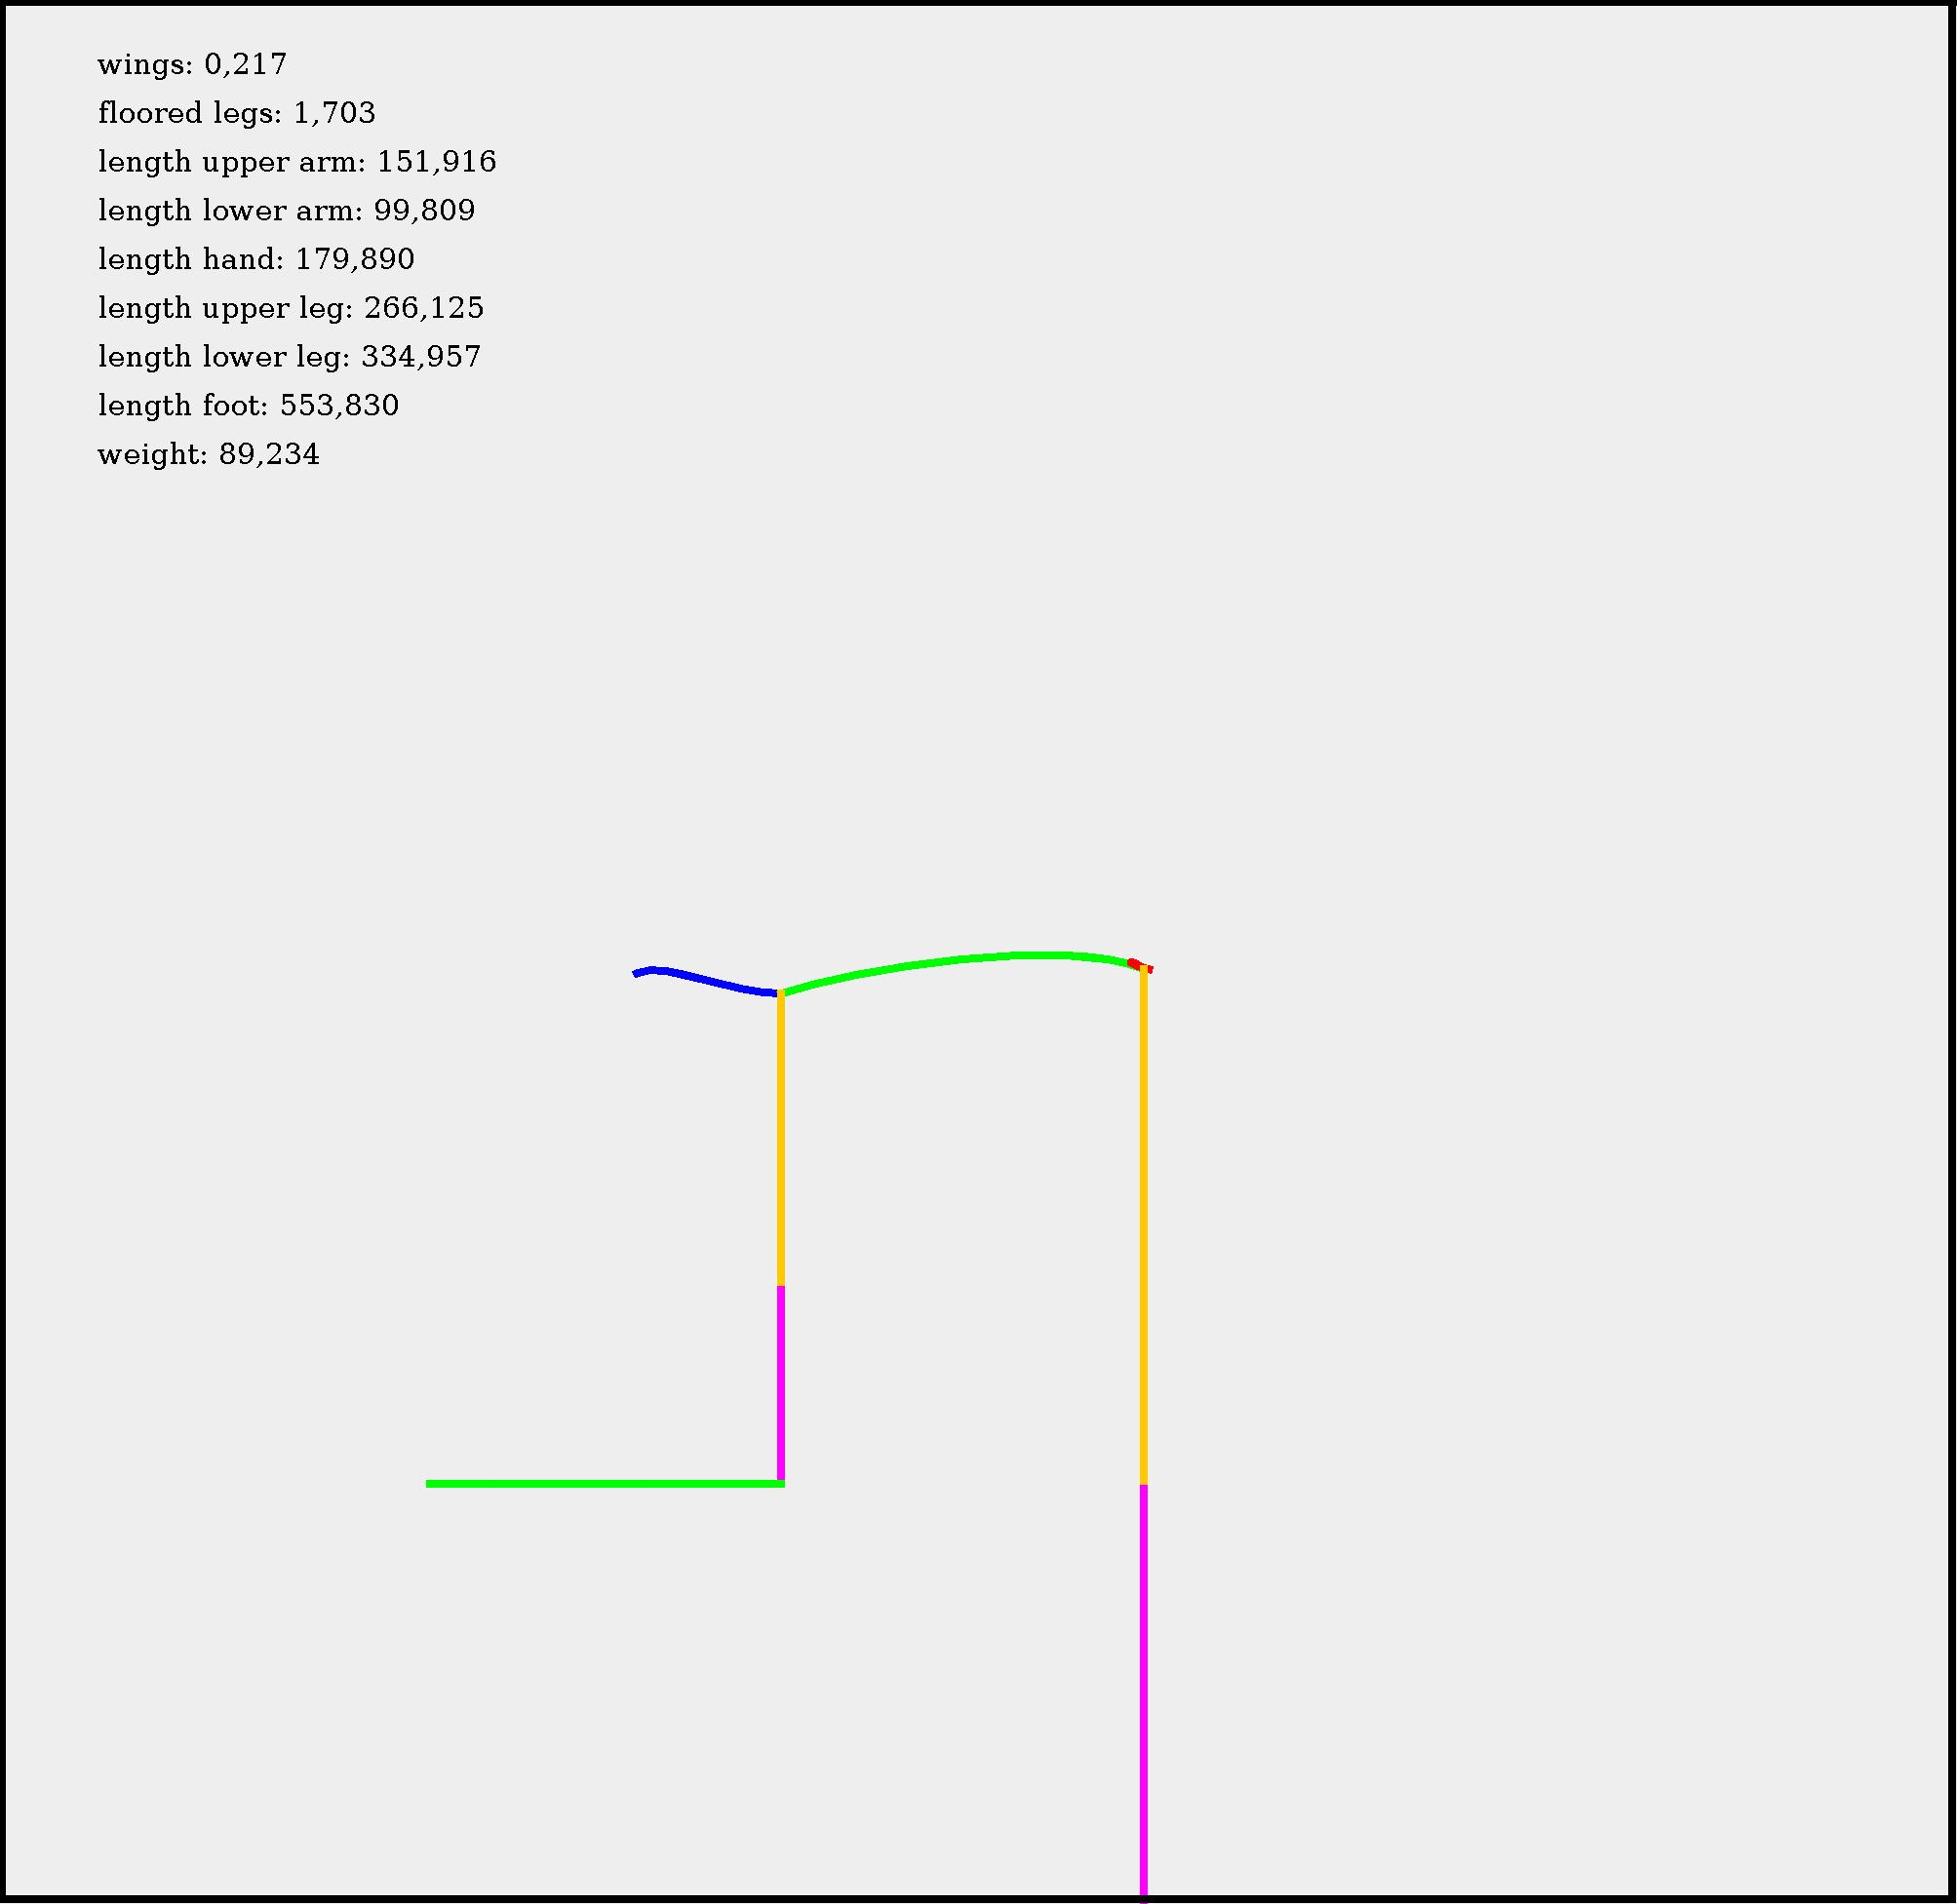
\includegraphics[width=0.5\textwidth]{../PCA/animal_reconstructions_log_weight_downscaled_wings_legs_and_weight/20EV/Frosch_Ausschnitt.jpg}}
  \qquad
  \subfloat[Eingabebild]{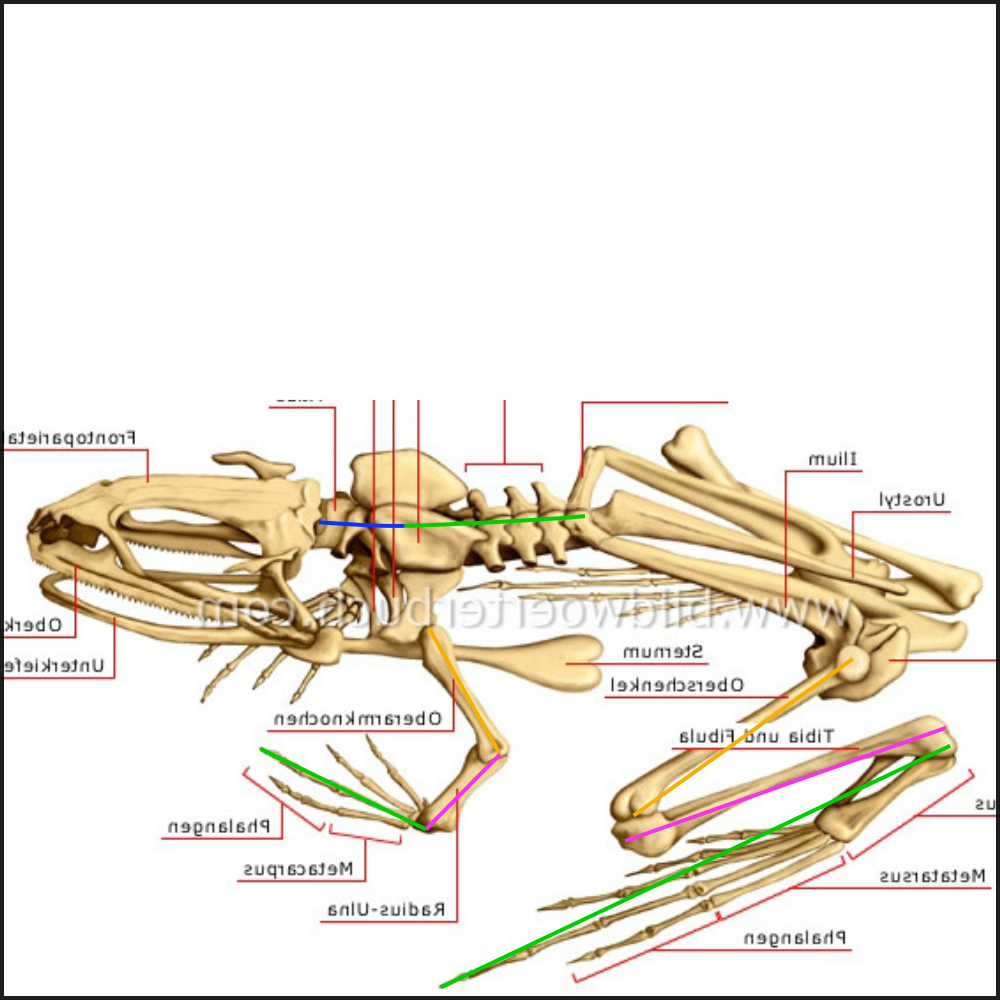
\includegraphics[width=0.5\textwidth]{../PCA/Skelettbilder/Frosch_farbig.png}}
  
  \caption{Frosch, Rekonstruktionen aus den größten $6$, $10$ und $20$ Eigenvektoren und das Eingabebild (d). Nicht visualisierte Dimensionen sind jeweils unter dem entsprechenden Bild angegeben. Zusätzlich zum Eingabebild erhobene Daten sind:
  \emph{Tierklasse} Amphibie, \emph{Flügel} $0$, \emph{Beine mit Bodenkontakt} $2$, \emph{Gewicht} $0,01$kg.}
  \label{frosch}
 \end{figure}

 Bei allen Eingabedimension, außer der Position der Wirbelsäule, kann man die Frage stellen, ob sie nötig sind, oder ob sie die Ergebnisse der PCA eher verschlechtern. Deshalb wurde ausprobiert verschiedene (Kombinationen von) Merkmalen wegzulassen. Die Ergebnisse unterscheiden sich aber nicht extrem von der PCA mit allen Daten. \\
 Leider gibt es keine gute Möglichkeit die Qualität der Ergebnisse der PCA zu messen. Man könnte den Unterschied zwischen den Eingabedaten und den Rekonstruktionen aus den Linearkombinationen der Eigenvektoren mit den größten Eigenwerten messen. Aber das liefert, durch das Fehlen von verschiedenen Dimensionen kein einheitliches Maß.
 Da jede Dimension dem Algorithmus, der später Skelette generieren soll, helfen könnte, wurde kein Merkmal verworfen.
 
 Außerdem gibt es die Möglichkeit die Eingabedaten in mehrere Mengen aufzuteilen und diese einzeln zu analysieren. Hierbei gibt es zunächst das Problem, dass sich dann die Anzahl der Datenpunkte noch weiter reduziert, was die Ergebnisse nicht mehr repräsentativ macht.
 Merkmale, die sich zur Unterteilung in Mengen anbieten würden, sind die diskreten, also \emph{Flügel} und \emph{Beine mit Bodenkontakt}. Sie sind auch klar als Cluster im Koordinatensystem der PCA ohne angepasste Skalierung zu erkennen (Abbildung \ref{projections_scales} a und b).
 Getestet wurde die Aufteilung anhand der Werte für die Flügel, da sich dadurch nur zwei Gruppen ergeben. Tatsächlich liefert sie bessere Rekonstruktionen aus den größten Eigenvektoren. Das liegt aber natürlich in erster Linie daran, dass die zu untersuchende Datenmenge, jeweils verkleinert wurde.
 
 Ein weiteres Problem daran die Daten in mehrere Mengen aufzuteilen ist, dass dann keine Skelette mehr erzeugt werden können, die zwischen den beiden Gruppen liegen. Tatsächlich scheinen aber die Datenpunkte, die "`zwischen"' den Gruppen erzeugt werden, relativ sinnvoll auszusehen.
 Auch das ist ein Argument dafür keine Aufteilung vorzunehmen.
 
 \todo{Beispiele für zufällig erzeugte Punkte}
 
 
 %-------------------------------------------------
 \section{Bedingte Verteilungen}
 \label{pca_conditions}
 
 
 Aus den Ergebnissen der PCA lassen sich sehr gut zufällige Skelette erzeugen. Es ist aber schwer gezielt Eigenschaften festzulegen.
 Der erste Schritt dies zu erreichen ist Eigenschaften, die so schon in den erhobenen Daten vorkommen, auf gewählte Werte festzulegen. Das können beispielsweise die Anzahl der Beine sein oder ob das Skelett Flügel haben soll.
 
 Dazu kann man, statt die ursprünglichen Daten und deren Verteilung zu verwenden, die entsprechenden bedingten Verteilungen bilden. Dazu muss der bedingte Mittelwert und die bedingte Kovarianzmatrix, wie in \cite{conditionalDistribution} (S.\ $116$ f.) beschrieben, bestimmt werden.
 
 Seien 
 \[x = \begin{pmatrix} x_1 \\ x_2 \end{pmatrix}, 
  \mu = \begin{pmatrix} \mu_1 \\ \mu_2 \end{pmatrix} \text{und } 
  \Sigma = \begin{pmatrix} \Sigma_{11} & \Sigma_{12} \\ \Sigma_{21} & \Sigma_{22} \end{pmatrix} \] 
 
 Der Zufallsvektor $x$ enthält $n$ normalverteilte Zufallsvariablen, $q$ Variablen im Vektor $x_1$ und $n - q$ in $x_2$. Die Einträge in $\mu$ sind die jeweils zugehörigen Mittelwerte und $\Sigma$ ist die Kovarianzmatrix. Die Verteilung für $x_1$ unter der Bedingung, dass $x_2 = b$ hat den Mittelwert $\bar{\mu}$ und Kovarianzmatrix $\overline{\Sigma}$ mit
 
 \[ \bar{\mu} = \mu_1 + \Sigma_{12} \Sigma_{22}^{-1} (b - \mu_2), 
    \overline{\Sigma} = \Sigma_{11} - \Sigma_{12} \Sigma_{12}^{-1} \Sigma_{21} \]
 
 Verwendet man nun $\overline{\Sigma}$ als Eingabe für die PCA, so erhält man nur noch Daten für Skelette unter den vorher festgelegten Bedingungen $b$. Zu beachten ist hier, dass die Eigenvektoren sich im Vergleich zur PCA ohne Bedingungen verändern. Falls man diese also zur Bestimmung eines Datenpunktes verwendet hat (\zb in einer Benutzeroberfläche), so müssen die Werte für die neuen Eigenvektoren neu ausgerechnet werden.
 
 % feste Werte variieren
 Erzeugt man nun in diesem bedingten Raum zufällige Beispiele, zeigt sich sehr deutlich, dass das Festlegen von nur einer Dimension auch die anderen Dimensionen stark einschränken kann. Legt man \zb die Anzahl der Beine fest, so haben die Skelette, die dann bedingt zufällig generiert werden, eine recht geringe Varianz. Das ist daran zu erkennen, dass der Verlauf der Wirbelsäule sehr ähnlich ist (siehe Abbildung \ref{spine_variance}a).\\
 Um das etwas zu umgehen, wird die Eingabe als Intervall aufgefasst, aus dem zufällig ein Wert gezogen wird. Legt der Benutzer \zb einen ganzzahligen Wert fest, so wird ein kleiner zufälliger Wert aufaddiert oder abgezogen. So wird nicht immer genau der gleiche Wert verwendet. Zwei Beispiele sind in den Abbildungen \ref{spine_variance} b und c gezeigt.
 
 \begin{figure}
  \subfloat[$0$ Flügel, ohne Anpassung]{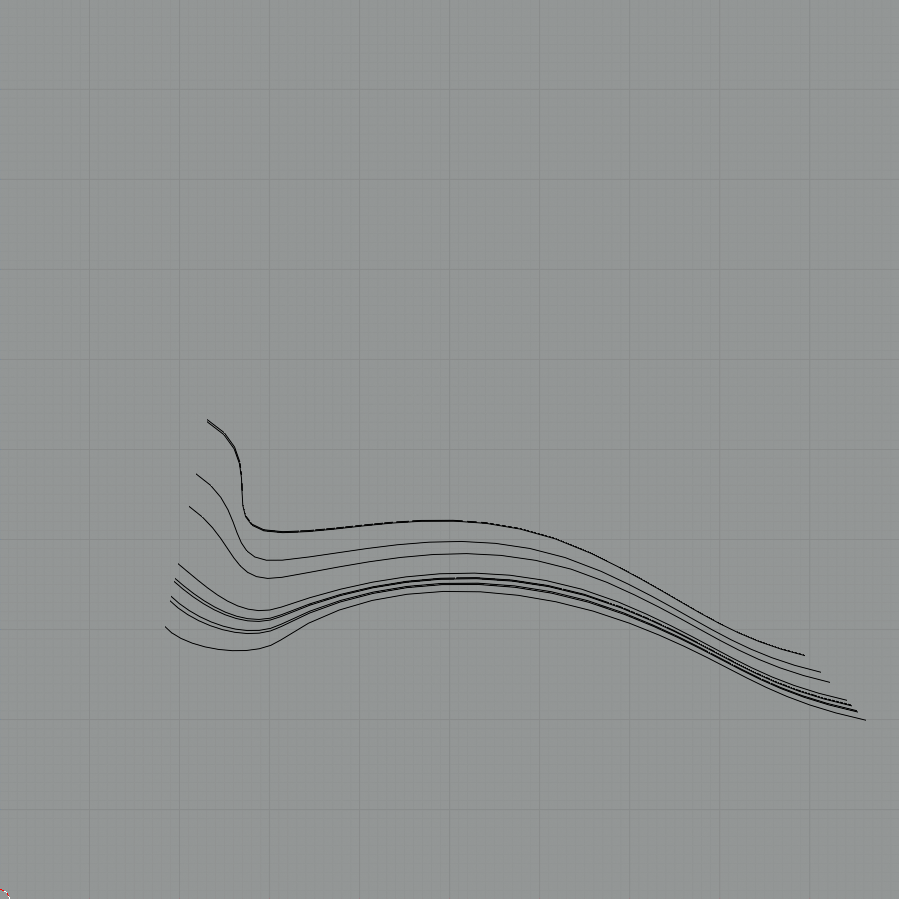
\includegraphics[width=0.3\textwidth]{graphics/0wings_withoutAdditionalVariance.png}}
  \qquad
  \subfloat[$0$ Flügel, mit Anpassung]{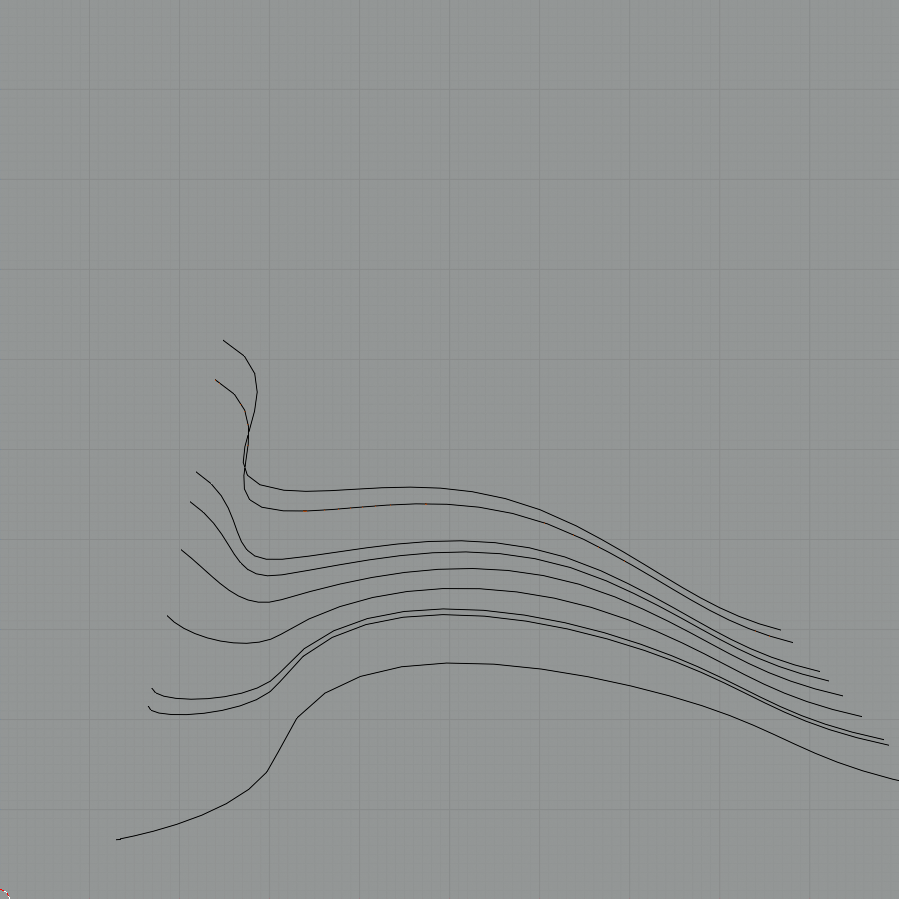
\includegraphics[width=0.3\textwidth]{graphics/0wings_withAdditionalVariance.png}}
  \qquad
  \subfloat[$1$ Paar Beine, mit Anpassung]{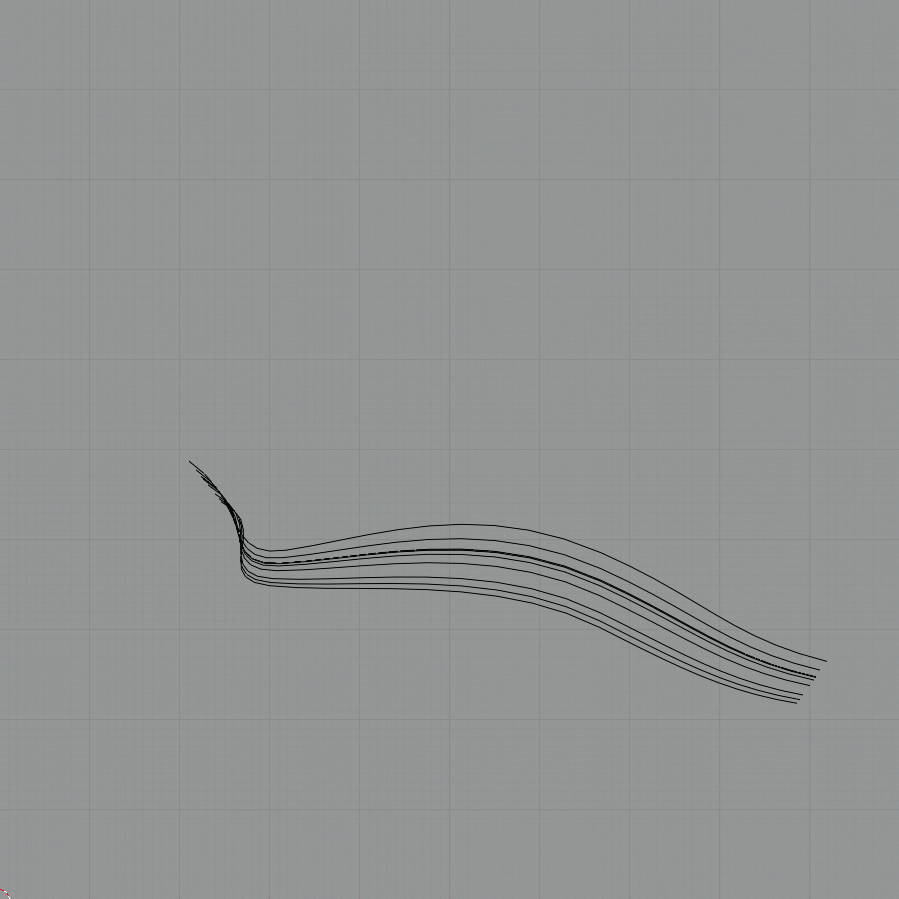
\includegraphics[width=0.3\textwidth]{graphics/1leg_withAdditionalVariance.png}}
  
  \caption{Jeweils $10$ bedingt zufällig generierte Wirbelsäulen. (a) und (b) ohne Flügel, (c) mit einem Paar Beine. In (b) und (c) wird ein zufälliger Wert aus $[-0.5, 0.5]$ auf die Bedingung (Flügel $= 0$ \bzw Beine $= 1$) aufaddiert.}
  \label{spine_variance}
 \end{figure}

 
 % Übergang Krokodil -> Fisch
 Schaut man sich nun die erzeugten Wirbelsäulen mit einem Paar tragender Beine an (Abbildung \ref{spine_variance}c), so liegen sie alle recht nah an der mittleren Wirbelsäule (Abbildung \ref{mean}).
 Das wirkt zunächst überraschend, da die meisten Tiere in den erhobenen Beispielen, die zwei Beine haben, Vögel sind. Sie haben eine Wirbelsäule, die hoch über dem Boden liegt und relativ aufrecht ist. Dann gibt es noch Känguru und Tyrannosaurus Rex. Bei ihnen liegt die Wirbelsäule ähnlich. Es muss aber auch einen Übergang von bodennahen Vierbeinern wie Krokodilen oder Fröschen über Zweibeiner zu Fischen ohne Beine geben. Nur gibt es dafür in der Natur eher wenige Beispiele. In den erhobenen Daten sind das nur der Seehund und die Ohrenrobbe.
 
 % Bedingungen an abgeleitet Werte
 Nun möchte man vielleicht Bedingungen an das zu generierende Skelett stellen, die nicht schon genau so in den erhobenen Daten repräsentiert sind. 
 Bedingungen an Dimensionen, die gar nicht erhoben wurden, können  entweder, unabhängig von der PCA, in den Ersetzungsregeln erzwungen werden, wie \zb die Anzahl der Flossen, oder sie müssen in die Erhebung eingefügt werden.
 
 Bedingungen, die schon implizit in den erhobenen Daten enthalten sind, sind beispielsweise die Schwanz- oder Halslänge. Um an sie Bedingungen stellen zu können, könnte man ebenfalls eine zusätzliche Dimension einfügen. Sie kann einfach aus den schon bestehenden Dimensionen errechnet werden. Dabei wäre aber das Problem, dass nur die Dimensionalität der Daten erhöht wird, nicht aber die eingegebenen Informationen. Es wären also mehr Eingabebeispiele nötig, nur dafür, dass die PCA eine offensichtliche Korrelation der Dimensionen erkennt.
 
 Die bessere Alternative ist die Eingabedimensionen der PCA umzuparametrisieren. Die Länge des Schwanzes in x-Richtung, ist \zb implizit in der Differenz der x-Koordinaten des ersten und letzten Kontrollpunktes der Bezièrkurve des Schwanzes enthalten. Ersetzt man nun den absoluten x-Wert des letzten Kontrollpunktes durch den Abstand in x-Richtung zum ersten Kontrollpunkt, so lässt sich die Schwanzlänge in x-Richtung ganz einfach als Bedingung an die PCA stellen. 
 
 % Schwanzlänge messen
 Betrachtet man nun konkret den Wunsch die Schwanzlänge festzulegen, ist das nicht ganz so einfach. Die Längen in x- und y-Richtung lassen sich zwar leicht festlegen, diese Längen sagen aber im Allgemeinen noch nicht viel über die tatsächliche Länge der Bezièrkurve aus. Verlangt man \zb eine Länge von $0$px für den Schwanz in x-Richtung, so haben die generierten Datenpunkte einen Schwanz der zwar auf gleicher Höhe beginnt und endet, aber trotzdem vorhanden ist und einen kleinen Bogen beschreibt. \todo{Beispielbild}
 Um die wirkliche Länge des Schwanzes zu messen, müsste man also noch mehr Aufwand in die Umparametrisierung stecken oder doch eine zusätzliche Dimension für die PCA in Kauf nehmen.
 
 

%-------------------------------------------
%-------------------------------------------
\chapter{Algorithmus zur Skelettgenerierung}

%-----------------------------------------------
\section{Generierung der einzelnen Extremitäten}
\label{section:extremity_generation}

Extremitäten werden zunächst danach unterschieden, ob sie Bodenkontakt haben sollen oder nicht.
Wenn nicht, dann sind es entweder Flossen, Arme oder Flügel:

\begin{itemize}
 \item Flossen: gerade nach hinten (orientiert an Welt-x-Achse)
 \item Arme: Oberarm gerade nach unten (orientiert an negativer Welt-y-Achse), Unterarm im $90^{\circ}$ Winkel nach vorne, Hand verlängert Unterarm 
 \item Flügel: spezielles Winkelintervall für jedes beteiligte Gelenk, daraus jeweils zufällig gewählte Winkel
\end{itemize}

% Beine mit iterativem Algo
Bei Extremitäten mit Bodenkontakt wird iterativ vorgegangen. Der allgemeinste Ansatz wäre hier inverse Kinematik zu verwenden. Das ist hier aber nicht nötig, da in jedem Schritt klar ist, wie die Winkel verändert werden müssen, dass der Endpunkt näher zum Boden kommt. \todo{Absatz über IK, lcp (linear complementary problem) (nicht Hauptaugenmerk / Ziel der Arbeit ist etwas anderes / reicht für Proof of Concept, bei Animationen muss große Maschinerie sowieso nochmal angeworfen werden)}\\
\todo{Absatz über Darstellung der Gelenke (auch mit zwei Freiheitsgraden), Problematik mit lokalen Winkelkonstraints vs. globalen Berechnungen für Abstand zum Boden}
Von der Startposition aus, werden die Winkel an den Gelenken in jedem Schritt jeweils so vergrößert oder verkleinert, dass sich der Punkt, der zum Schluss den Boden berühren soll, sich der Bodenoberfläche nähert. Ob die Winkel jeweils vergößert oder verkleinert werden sollen, wird bestimmt, indem die Ausrichtung des Kindelements mit der y-Achse des Weltkoordinatensystems verglichen wird. Soll der Endpunkt der Extremität dem Boden nähern, so wird der Winkel so verändert, dass die Ausrichtung des Kindelements sich der Senkrechten nähert. Wenn nicht, so wird der Winkel in die entgegengesetzte Richtung verändert. \todo{das passiert aber nicht}

% Tweaks
Je nach Ausgangsposition sieht das Ergebnis aber nicht unbedingt natürlich aus. Zum Beispiel kann es passieren, dass das Fußgelenk nicht gedreht wird, also der Fuß das Schienbein einfach verlängert und die Spitze des Fußes Bodenkontakt hat. Wenn dann die Oberseite des Fußes näher am Boden ist als die Unterseite, dann ist das keine sinnvolle Position.
Um so etwas zu verhindern, wird die Startposition der Extremität so gewählt, dass alle Gelenke stark angewinkelt sind. \todo{Abbildung}
Außerdem wird während der Iteration verboten, dass Knochen unterhalb der Bodenhöhe enden.
\todo{Zweiter Freiheitsgrad an Hüft- und Schultergelenk macht es schwieriger, da Winkel, je nach Winkel der anderen Richtung, vergrößert oder verkleinert werden muss um den Boden zu erreichen. Weggelassen. Bei mehr Anforderungen doch IK verwenden.}

% Änderung der Winkel und Wahrscheinlichkeiten
In jedem Schritt werden die Winkel um eine bestimmte Gradzahl verändert. Diese Gradzahl verkleinert sich mit jedem Schritt bis zu einer Minimalgröße. Zu Beginn werden die Winkel stark verändert um die grobe Ausrichtung des Beines festzulegen und in den kleiner werdenen Schritten wird die Extremität genauer ausgerichtet, so dass der Endpunkt zum Schluss auf dem Boden steht.
Zusätzlich wird nicht in jedem Schritt jeder Freiheitsgrad jedes Gelenks verändert. Für jeden Freiheitsgrad wird eine Wahrscheinlichkeit (kleiner als eins) festgelegt, dass dieser ausgewählt wird. Dadruch können bestimmte Richtungen oder Gelenke priorisiert werden um ein besseres Ergebnis zu erzielen. \todo{Was sind die guten Einstellungen? bzw braucht man dise Wkten überhaupt?}
\todo{Konkrete Einstellungen erwähnen (in Implementierungsdetails?)}

%--------------------------------------
\section{Ansatzpunkte für Extremitäten}

Ansatzpunkte für Extremitäten sind natürlich zunächst der Hüftgürtel und der Schultergürtel. Um auch die Generierung fantastischer Tiere zu ermöglichen, ist es aber Möglich dies zu erweitern.

Eine einfache Möglichkeit ist hier zunächst die Anzahl der möglichen Extremitätenpaare von zwei auf vier zu erhöhen, indem einfach an der Hüfte und der Schulter jeweils zwei Paare ansetzen dürfen. Dafür wurden einfach an der Hüfte \bzw der Schulter mehrere Gelenke mit ein wenig Abstand angelegt, an denen Extremitäten ansetzen können.
Flügel und Arme dürfen hierbei weiterhin nur an der Schulter ansetzen, Beine und Flossen an beiden Stellen. Der Grund dafür ist, dass die meisten generierten Skelette seltsam wirken, wenn an der Hüfte Flügel oder Arme ansetzen und dafür an der Schulter Beine beginnen. Das liegt daran, dass existierende Tiere mit Flügeln oder Armen ihren Schwerpunkt im hinteren Bereich haben und sie auf den Hinterbeinen stehen.

% mehr Extremitätengürtel auf dem Rücken
Eine Überlegung war auch zwischen Schulter und Hüfte weitere Extremitätengürtel anzubringen. Das stellt sich aber als schwierig heraus. Die Wirbelsäule ist zwischen Hüfte und Schulter nach oben geschwungen und im Bauchraum befinden sich die meisten Organe des Tieres. Ein zusätzlicher Extremitätengürtel würde den Bauchraum einschränken. Außerdem wirkt dann auch die nach oben geschwungene Wirbelsäule anatomisch seltsam.
"`Verdoppelt"' man die Schwingung der Wirbelsäule und hängt einfach einen weiteren Rücken hinten oder vorne an, so wirkt es ebenso seltsam, da dann die "`Höcker"' der Wirbelsäule für das Tier wahrscheinlich nicht wirklich ein Vorteil sind und nur die Fortbewegung erschweren.

% zweiter Schultergürtel
Eine weitere Idee, die auch umgesetzt wurde, ist, eine Art Zentauren zu ermöglichen. Hat das Tier einen Hals, der lang genug ist, kann darauf ein weiterer Schultergürtel kurz unterhalb vom Kopf angebracht werden. An diesem Schultergürtel dürfen dann keine alle Arten von Extremitäten außer Beinen ansetzen. Das wirkt tatsächlich meist auch anatomisch einigermaßen sinnvoll.


%--------------------------------
\section{Knochenmodelle einfügen}

Zunächst wird jeder terminale Knochen durch seine Bounding Box dargestellt. Diese Boxen lassen sich aber leicht durch die 3D-Modelle der entsprechenden Knochen ersetzen. Dazu müssen die 3D-Modelle nur im .obj-Format vorliegen und folgenden Bedingungen entsprechen:

Das Modell ist korrekt an den Achsen ausgerichtet und so verzerrt, dass es einen Würfel mit 1(m) Kantenlänge in jeder Richtung möglichst gut ausfüllt.

Lässt man es hierbei bewenden, so ist es relativ schwierig herauszufinden wie man die einzelnen Knochen skalieren muss, dass sie an den Gelenken gut zusammenpassen. Außerdem ist es aufwändig herauszufinden wo die Gelenke an den Knochen ansetzen.

Setzt man sich dagegen etwas über den Gedanken der "`Bounding Box"' hinweg, so kann die Positionierung und Skalierung einfacher werden. Hier wurden, je nach Knochen, einige der folgenden Punkte umgesetzt. \todo{Beispielbilder}
\begin{itemize}
 \item Kleine Fortsätze, die nicht wirklich zur (optischen) Größe des Knochens beitragen, \zb die Fortsätze der Wirbel, ragen aus der Bounding Box heraus.
 
 \item Kantenlängen, die von "`außen"' vorgegeben werden, sind genau auf die Kantenlänge der Box skaliert (also 1). So beispielsweise die x-Länge der Wirbel, die auf der Wirbelsäule genau aneinender stoßen sollen. Dies können aber auch Längen sein, nur einen Teil des Knochens betreffen. Der Beinabstand an der Hüfte ist \zb kleiner als die komplette Breite der Hüfte. Es ist aber einfacher den Beinabstand anzugeben, als die Hüftbreite. Auch die Skalierung der Hüfte in x-Richtung ist zunächst nicht klar, aber wenn die Breite der zugehörigen Wirbel gegeben ist, ist auch klar, wie breit die Hüfte sein soll. Deshalb ist die Hüfte in x-Richtung so skaliert, dass der Teil, an dem der Wirbel ansetzt, schon die komplette Kantenlänge des Würfels ausfüllt. Bei Gelenken, die von der Breite her zusammenpassen sollen, ist dies auch sehr hilfreich. Aber das führt natürlich auch dazu, dass die "`Bounding Box"' nicht mehr viel mit der resultierenden Größe des Knochens zu tun haben muss.
 
 \item Kantenlängen, die nicht vorgegeben werden, sind einfacher passend zu bestimmen, wenn sie nicht komplett unabhängig von den anderen Raumrichtungen sind. Ist \zb die x- und y-Skalierung eines Knochens vorgegeben, und die Skalierung in z-Richtung soll nur möglichst gut dazu passen, so ist es sinnvoll, das 3D-Modell schon so zu speichern, dass die z-Richtung von einer der anderen Richtungen abhängt. Tut man dies nicht, so führt das relativ leicht dazu, dass die Knochen grundlos verzerrt werden.
\end{itemize}

Liegen die Modelle in diesem Format vor, können sie einfach eingelesen werden und anhand der Skalierung der Bounding Box skaliert werden.
Hier wurden vor allem Modelle von menschlichen Knochen verwendet, da sie leichter verfügbar sind. Manche Knochen sind jedoch auch von anderen Tieren. Das führt \zb bei dem verwendeten Unterarmknochen des Pferdes dazu, dass er etwas überdimensionierte Fortsätze am Ellenbogen bekommen, wenn man ihn großskaliert. Das liegt daran, dass dieser Knochen beim Pferd eigentlich relativ kurz ist.

% Ausrichtung der Knochen
Eine Schwierigkeit daran Modelle in der oben genannten Form herzustellen ist, dass nicht unbedingt sofort klar ist, wie die Knochen ausgerichtet werden müssen. Die Hüfte muss \zb so ausgerichtet werden, dass der Anfangs- und Endpunkt der durchgehenden Wirbelsäule auf gleicher Höhe liegen, damit nachfolgende Wirbel auch richtig anschließen. (Das funktioniert natürlich nur, weil die Wirbelsäule an der Stelle der Hüfte quasi gerade ist.) \todo{wg Lizenz Pferdehüfte verwendet, die nicht mit Wirbelsäule verwachsen ist}
Auch die Positionierung der Rippen und des Oberarms in Kombination mit dem Unterarm ist anspruchsvoll. Dabei hilft es 3D-Modelle zu haben, in denen die anderen Knochen auch schon vorhanden sind, um sich die Ausrichtung abzuschauen. Außerdem können Bilder von Skeletten zu Rate gezogen werden. Und zuletzt muss man die genaue Positionierung einfach testen.

% Gelenke korrekt ausrichten
Zusätzlich muss beachtet werden wie die Knochen aneinander anschließen \bzw wie sie für die entsprechenden Gelenke korrekt positioniert sind. Das erfordert etwas "`finetuning"'. Für jeden Knochen sind dafür in Abhängigkeit zur Bounding Box zwei Offsets gespeichert: das Offset zu dem Gelenk, das ihn mit seinem Elternknochen verbindet und das Offset zu dem Gelenk, das ihn mit seinem Kindknochen verbindet (oder mehrere, falls vorhanden). Dies sorgt dafür, dass die Positionierung der Knochen stimmt, egal wie groß sie sind. Ist ein Knochen sehr groß und ein anschließender sehr klein (oder anders herum), so kommt es natürlich trotzdem vor, dass die Gelenke nicht wirklich ineinander passen. Für solche Situationen bräuchte man verschiedene 3D-Modelle, die je nach Gegebenheit eingesetzt werden.

% Köpfe
Da der Kopf \bzw der Schädelknochen im Gegensatz zu anderen Knochen bei Wirbeltieren sehr stark variiert, ist es sinnvoll mehrere Schädelknochen zur Auswahl zu haben. Geht die Menge an verfügbaren Schädelknochen über "`Tier mit Flügeln"' und "`Tier ohne Flügel"' hinaus, so ist es außerdem sinnvoll die Auswahl des passenden Schädelknochens dem Nutzer zu überlassen.

% Hände und Füße
Bei Händen und Füßen ist das Problem ebenso, dass es sehr viele verschiedene Ausprägungen davon gibt. Hier lassen sie sich jedoch grob nach Extremitätentyp unterscheiden. Diese Unterscheidung kann aber beliebig fein sein. Hier wurde nur nach Flügel, Flosse \todo{?} und Extremität mit Bodenkontakt unterschieden. Und bei Extremitäten mit Bodenkontakt wurde nochmals danach unterschieden wie flach der Fuß oder die Hand auf dem Boden aufkommt (bei weniger als $45^\circ$ ist es eine menschliche Hand, sonst ein Huf). \todo{ggf. an Implementierung anpassen}

% mehrere Extremitäten an einer Schulter/Hüfte
Setzten mehrere Extremitäten an einer Schulter oder einer Hüfte an, so ist ein "`normales"' Modell der Schulter/Hüfte nicht mehr ausreichend, da nicht genug Gelenke vorhanden sind. Dieses Problem wurde an der Schulter so behoben, dass einfach mehrere Schulterblätte mit einem gewissen Abstand generiert wurden. Für die Hüfte wurde ein kombiniertes 3D-Modell aus zwei einzelnen Hüften erstellt, an dem nun zwei Gelenke vorhanden sind.

%------------------------
\section{Ergebnisskelette}

\begin{itemize}
 \item Einheiten der PCA für Koordinaten $[0, 1000]$, deshalb sind die Wirbelsäulen der generierten Skelette auch in diesem Rahmen. Blender interpretiert eine Einheit als $1$m. Deshalb wirken sie sehr groß.
 
 \item Die Abmessungen der Knochen in die verschiedenen Richtungen ist bei den meisten Knochen relativ beliebig gewählt und oft auch immer gleich (außer bei Längen, die von PCA vorgegeben sind). Dafür gibt es keine biologische oder anatomische Grundlage. Man könnte hier sicherlich noch mehr machen (mehr Zufall, mehr anatomisch korrekt etc.)
 \todo{in Implementierungsdetails aufzählen was an Abmessungen alles beliebig (oder auch weniger beliebig) festgelegt wurde.}
\end{itemize}



%--------------------------------
%--------------------------------
\chapter{Implementierungsdetails}
\label{chapter:implementation_detail}

%---------------------------
\section{Programmiersprache}

\begin{itemize}
 \item Rust: nicht geeignet, da Datenstrukturen die zyklische Referenzen auf veränderbare Objekte verwenden nicht oder nur kompliziert umsetzbar sind.
 \item Java: scheint gut zu funktionieren. Es gibt Bibliotheken zum im-/exportieren von obj-Dateien und Unterstützung für OpenGL\\
 Außerdem gibt es Bibliotheken, die PCA (\bzw Kovarianzmatrizen \etc) unterstützen und JavaView um objs darzustellen
\end{itemize}


%---------------------
\section{Dateiformate}

\begin{itemize}
 \item Einfachstes Format (nur für die Darstellung von 3D-Objekten ohne Zusatzinformationen): obj
 \item Erster Schritt: einfaches .obj erzeugen und mit Blender darstellen; einfach Knochen als Bounding Box darstellen, später Verwendung von OpenGL mit vertex shadern \etc (Plan erwähnen? wurde ja doch nicht gemacht\dots)
 \item Jeder Editor geht mit Muskeln und Gelenken anders um. Gibt es ein Dateiformat, das nicht speziell zu einem Editor gehört, dass Bedingungen an die Rotation von Gelenken speichern kann?
 \item Eigenes Format erzeugen? Dann bräuchte man Plugins um es in verschiedenen Editoren laden zu können. Viel verwendeter Editor: Houdini (kostenlos für Studenten aber nicht Open Source). Oder selbst darstellen (siehe Interaktivität).
\item Vorschlag von Jo: "`Memory dumps"', also direkt die structs aus dem speicher auf platte rausschreiben. Am besten wenn sie am Stueck liegen mit einem fwrite() und zurücklesen mit einem fread(). Es ist nuetzlich dazu am Anfang der Datei ein bisschen Metadaten zu speichern (magic number, version, array size etc).
\end{itemize}

%- - - - - - - - - -
\subsection{OpenSim}

\begin{itemize}
 \item \url{https://simtk-confluence.stanford.edu:8443/display/OpenSim/OpenSim+Documentation}
 \item Open Source Software Platform für die Modellierung uns Simulation von Menschen, Tieren, etc.\\
 aber vor allem gedacht zur Auswertung von experimentellen Daten
 \item Import von .obj Dateien möglich. Außerdem zusätzliche Daten wie Winkel von Gelenken über .mot oder .sto Dateien (eigenes Format von OpenSim, siehe \url{https://simtk-confluence.stanford.edu:8443/display/OpenSim/Preparing+Your+Data})
 \item Export in andere Dateiformate nicht möglich (?)
 \item für Download und Zugang zur "`Community"' Account nötig
 \item für Windows und Mac OS (Linux Support gibt es auch, ist aber schwieriger: \url{https://simtk-confluence.stanford.edu:8443/display/OpenSim/Linux+Support})
\end{itemize}


%- - - - - - - -
\subsection{OBJ}

\begin{itemize}
 \item Beschreibung des Formats: \url{https://www.fileformat.info/format/wavefrontobj/egff.htm}
 \item Erzeugung mit Rust: obj\_exporter \url{https://docs.rs/obj-exporter/0.2.0/obj_exporter/index.html}
 \item Erzeugung mit Java: javagl Obj \url{https://github.com/javagl/Obj}, unterstützt auch Umwandlung von obj-Daten in Daten, die direkt für vertex buffer objects in OpenGL verwendet werden können
 \item Reicht wahrscheinlich für die ersten Dinge aus. Finetuning wird sowieso mit anderer Software gemacht
\end{itemize}

%- - - - - - - -
\subsection{FBX}

\begin{itemize}
 \item Verwendung am besten über Autodesk FBX SDK für C++. 
 \item Dokumentation: \url{http://help.autodesk.com/view/FBX/2019/ENU/} und \url{http://docs.autodesk.com/FBX/2014/ENU/FBX-SDK-Documentation/index.html}
 \item Es gibt auch fbxcel, eine FBX library für Rust. Ist aber relativ low level und nicht ganz offensichtlich wie zu verwenden.
 \item Einschränkungen für Gelenke können in FBX nicht gespeichert werden \url{http://docs.autodesk.com/FBX/2014/ENU/FBX-SDK-Documentation/index.html?url=cpp_ref/class_fbx_constraint.html,topicNumber=cpp_ref_class_fbx_constraint_htmlc57a3f99-513a-44a0-a24f-445e9077c99f}
\end{itemize}

%- - - - - - - - - -
\subsection{Alembic}

\begin{itemize}
 \item \url{www.alembic.io}
 \item Wird u.a. dafür verwendet Knochen (+ Animationen) in Ziva zu importieren
 \item Es kann mit Python (PyAlembic) und C++ verwendet werden.\\
 PyAlembic Doku: \url{http://docs.alembic.io/python/examples.html#pyalembic-intro}\\
 C++ API Refernce (enthält sehr wenig Infos): \url{http://docs.alembic.io/reference/index.html}
 \item Für Rust gibt es keine Bibliothek (?)
\end{itemize}


%----------------------------
\section{Aufbau der Software}

\begin{itemize}
 \item ein Wort zur Softwarearchitektur?
 \item Erweiterbarkeit der Software?
\end{itemize}


%-----------------------------
\section{Zufall}

Linearer Kongruenzgenerator reicht für Zufallszahlen aus, da nur wenige erzeugt werden (erkennbare Muster entstehen erst bei mehr Zufallszahlen) \todo{erwähnen?}


%--------------------------------
\section{Transformationsmatrizen}
\label{implementation_detail_matrices}

\todo{Recherchiere warum rechtshändige Koordinatensysteme bzw. konsistene Koordinatensysteme wichtig sind (back face culling, Rotationsrichtung der Matrizen bei positiven Winkeln)}

Jedes Element im Skelett speichert, relativ zu seinem Elternelement, die Position des Ursprungs seines Koordinatensystems. Um den Überblick über die Transformationsmatrizen bzw. Abbildungen behalten, die vom einen ins andere Koordinatensystem umwandeln, hier zwei Übersichtsgrafiken:
\todo{Erzeugung von Elementen auf der Wirbelsäule mit gegebener Weltposition + gespiegelte Elemente}

\begin{figure}
 \centering
 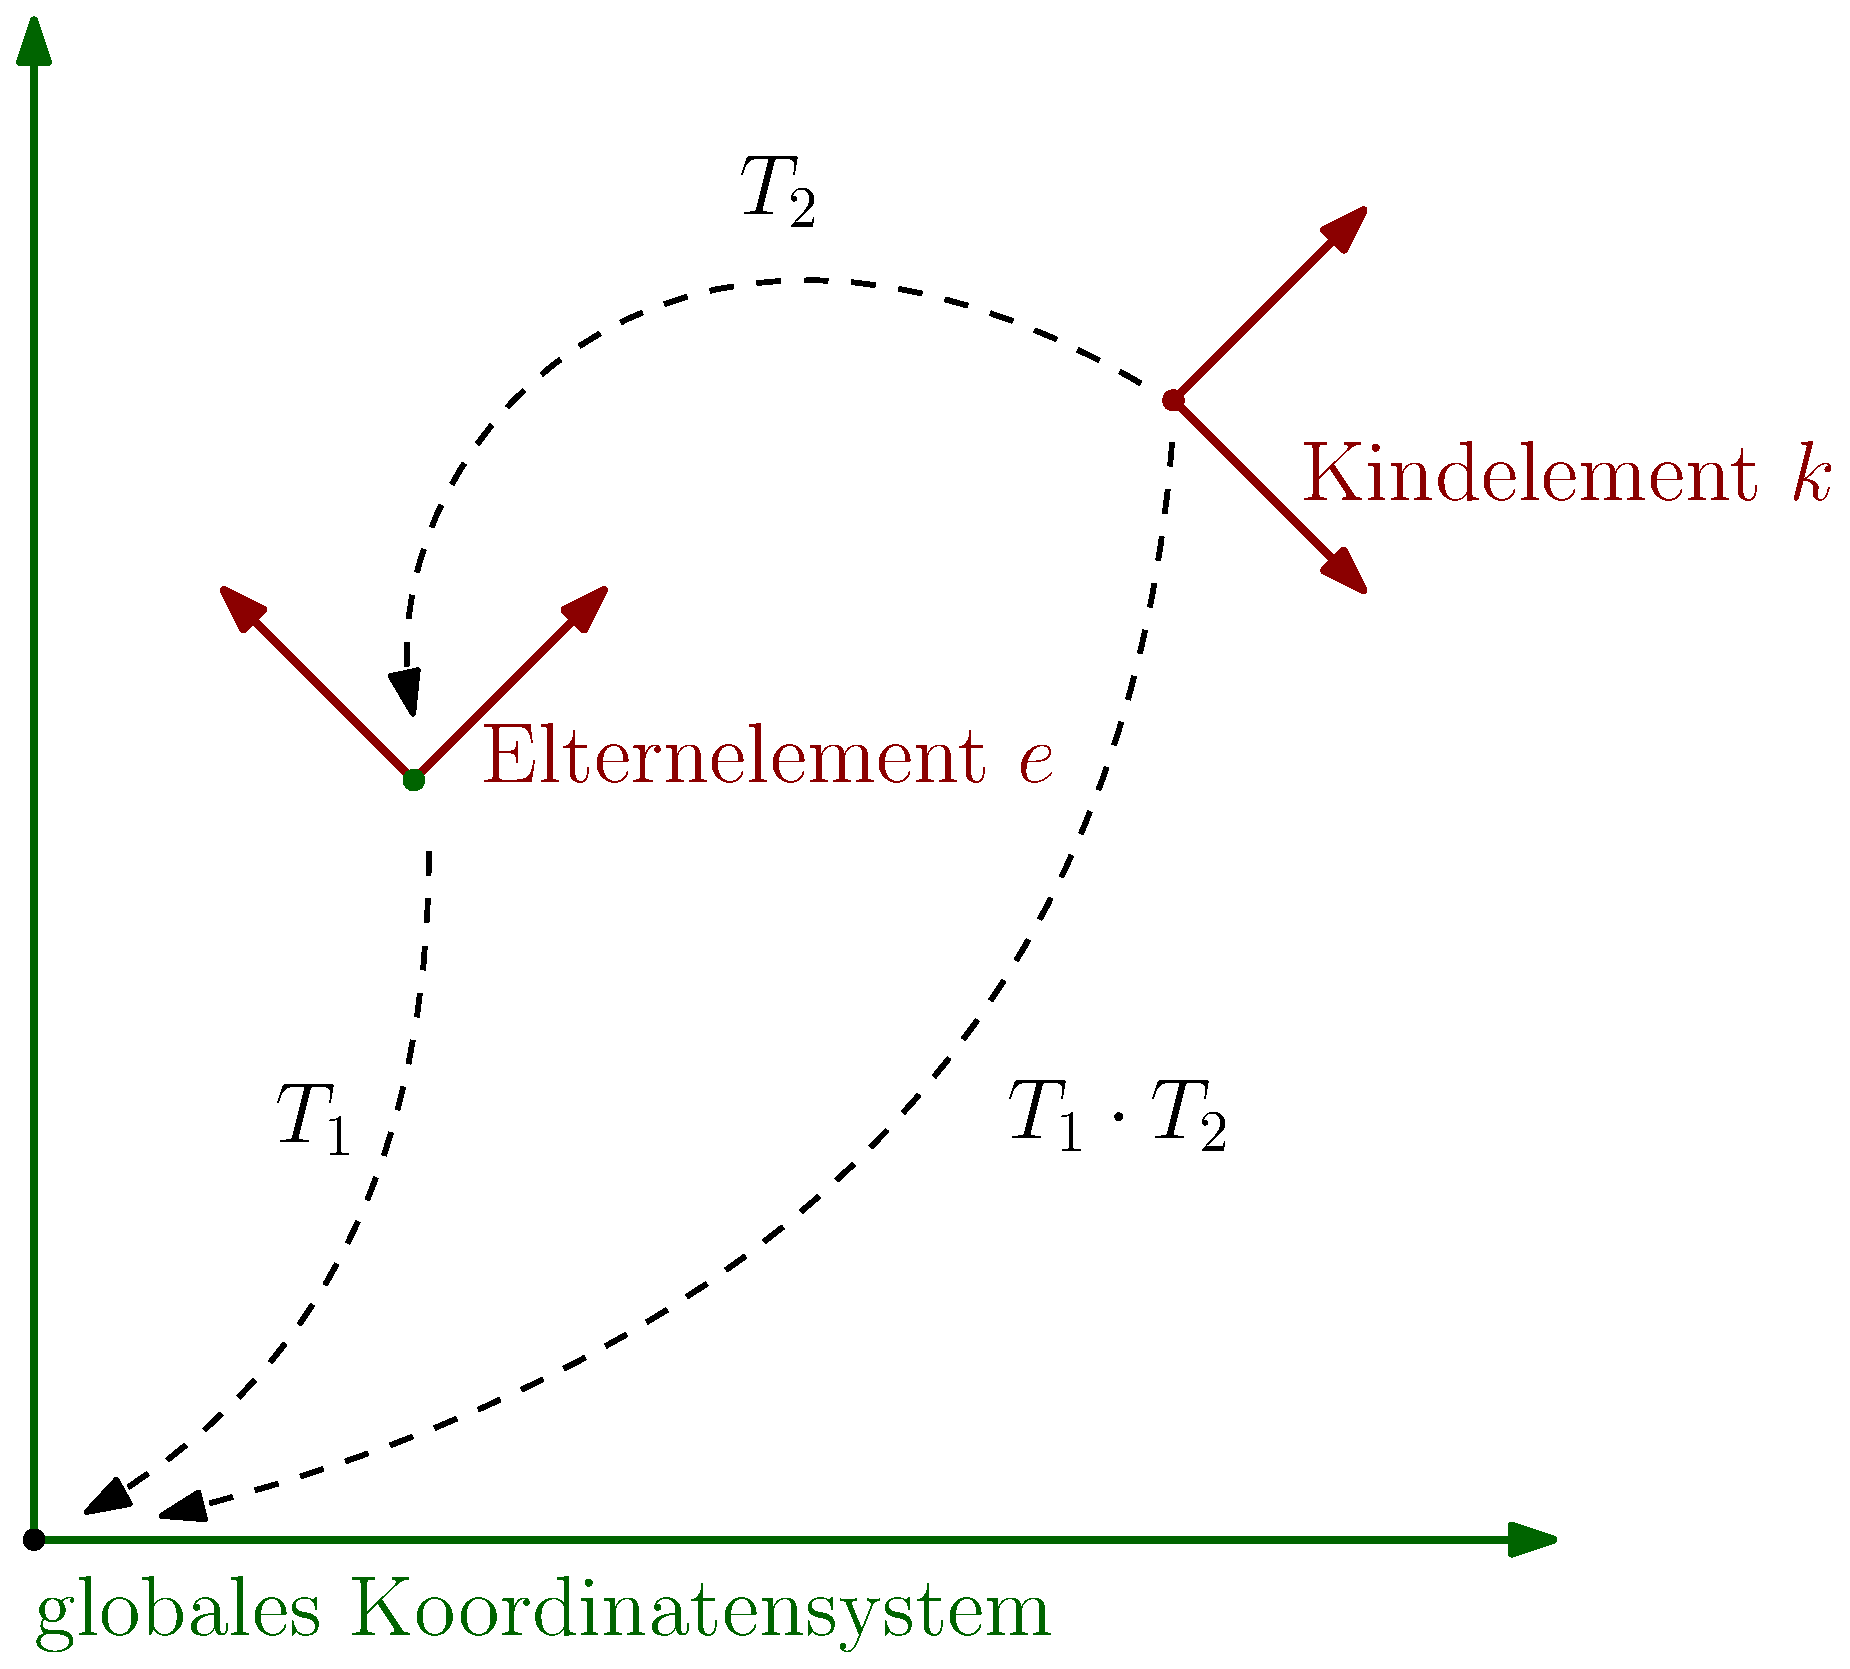
\includegraphics[width=0.6\textwidth]{graphics/transformation_matrices.eps}
 \caption{Gegeben sei das Element $e$. Die Abbildung, die die lokalen Koordinaten von $e$ in globale Koordinaten umrechnet sei $T_1$.
 Jedes Kindelement $k$ von $e$ speichert eine Transformationsmatrix $T_2$, die angibt wo der Ursprung des Koordinatensystems von $k$ relativ zum Koordinatensystem von $e$ liegt. Will mann nun Koordinaten von $k$ in globale Koordinaten umrechnen, benötigt man die Abbildung $T_1 \cdot T_2$.}
\end{figure}

\begin{figure}
 \centering
 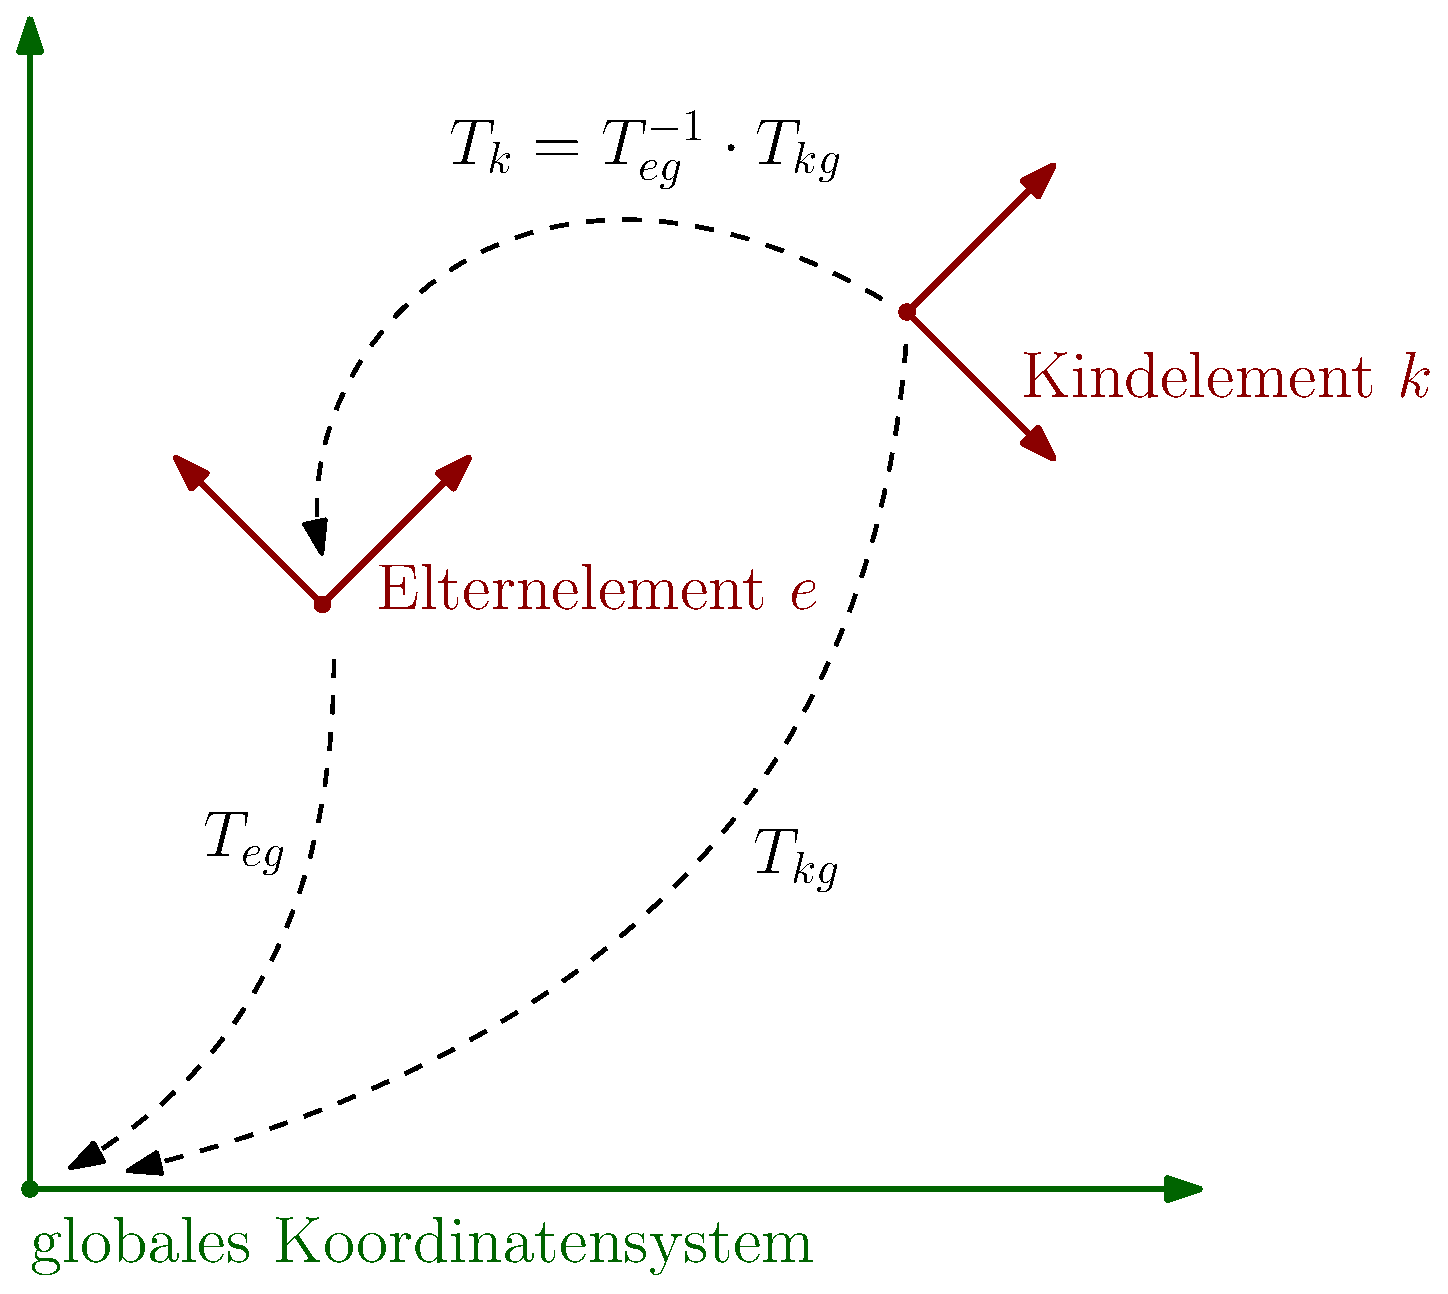
\includegraphics[width=0.6\textwidth]{graphics/transformation_matrices_spine.eps}
 \caption{Will man ein Element $k$ erzeugen, das Kindelement von $e$ ist und dessen globale Koordinaten bekannt sind, muss man die Abbildung berechnen, die die relative Position von $k$ angibt. Seien $T_1$ und $T_2$ jeweils die Transformationen in das globale Koordinatensystem von $e$ \bzw $k$. Dann ist die gesuchte Abbildung $T_1^{-1} \cdot T_2$.}
\end{figure}


%------------
\section{PCA}
\label{implementation_detail_pca}

Die Bilder der Skelette wurden folgendermaßen für die Datenerhebung vorbereitet:
 
 \begin{enumerate}
  \item Zuschneiden des Bildes, so dass möglichst nur das Skelett mit wenig Rand außen herum zu sehen ist.
  \item Einfügen in eine $1000 \times 1000$ Pixel große Bildumgebung.
  \item Verschieben innerhalb der Bildumgebung an den unteren Rand und horizontal in die Mitte.
 \end{enumerate}

 Ist das geschehen kann die Lage der Wirbelsäule und die Länge der Knochen der Extremitäten annotiert werden.
 
%- - - - - - - - - - - - - - - - -
\subsection{Annotation der Bilder}

Die Annotation der Bilder wurde per Hand mit dem Programm Inkscape\footnote{Programm zum erstellen und bearbeiten von Vektorgrafiken, \url{https://inkscape.org/de}} durchgeführt. Für jedes zu markierende Element wurde eine Strecke oder eine Bézierkurve eingefügt und mit einem vorher festgelegten Namen benannt. Diese Elemente wurden dann durch Inkscape als Pfade in der erzeugten svg-Datei gespeichert. Aus dieser Datei wurden dann automatisiert die eingetragenen Pfade mit ihren Koordinaten ausgelesen.

Folgende Details sind wichtig zu beachten, damit dieser Vorgang reibungslos abläuft. 
\begin{itemize}
 \item Man kann in Inkscape einstellen, dass Koordinaten immer absolut angegeben werden. Das ist sinnvoll um die Koordinaten leichter auslesen zu können.
 \item Der Ursprung des Koordinatensystems in Inkscape ist unten links, im svg-Format ist er aber oben links.
 \item Ebenen sollten in Inkscape nicht verschoben sein, sonst verschieben sich mit ihnen auch die Koordinaten.  
\end{itemize}

%- - - - - - - - - - - - - - - - - - - - - - - - - - - - - - - -
\subsection{Anpassung der PCA-Ergebnisse zur Weiterverarbeitung}

\begin{itemize}
 \item Um Wirbelsäule aus PCA Daten differenzierbar zu machen, wurden jeweils der vorletzte und der zweite Punkt von Hals und Rücken \bzw Rücken und Schwanz um den Kontaktpunk um den gleichen Winkel in gegensätzliche Richtungen gedreht, damit beide Bézierkurven an dem Kontaktpunkt die gleiche Steigung haben. \todo{beste Lösung?}
 \item An den Kontakpunkten der Wirbelsäulenteile ist die Steigung nicht unbedingt gleich (die Wirbelsäule als ganzes ist nicht $C^1$). Deshalb müssen vor der Weiterverwendung die jeweils nächsten Kontrollpunkte nach dem Kontakpunkt verschoben werden. Das wurde hier so gemacht, dass die zu verschiebenden Kontrollpunkte um den Kontakpunkt in gegensätzliche Richtungen rotiert wurden. Beide werden um den gleichen Winkel rotiert (siehe Abbildung \ref{smooth_spine}). Grundsätzlich könnten die Kontrollpunkte beliebig auf der Tangente des Kontaktpunkts platziert werden (rot im Bild) um eine übereinstimmende Steigung zu bekommen. Um den Verlauf der Wirbelsäulenteile möglichst wenig zu verändern ist es von Vorteil auch die Kontrollpunkte möglichst wenig zu verschieben. Man könnte die Punkte \zb auch senkrecht auf die Tangente projizieren. Welches Verfahren angewendet wird, ist jedoch nicht von großer Bedeutung. 
\end{itemize}

\begin{figure}
 \subfloat[vorher]{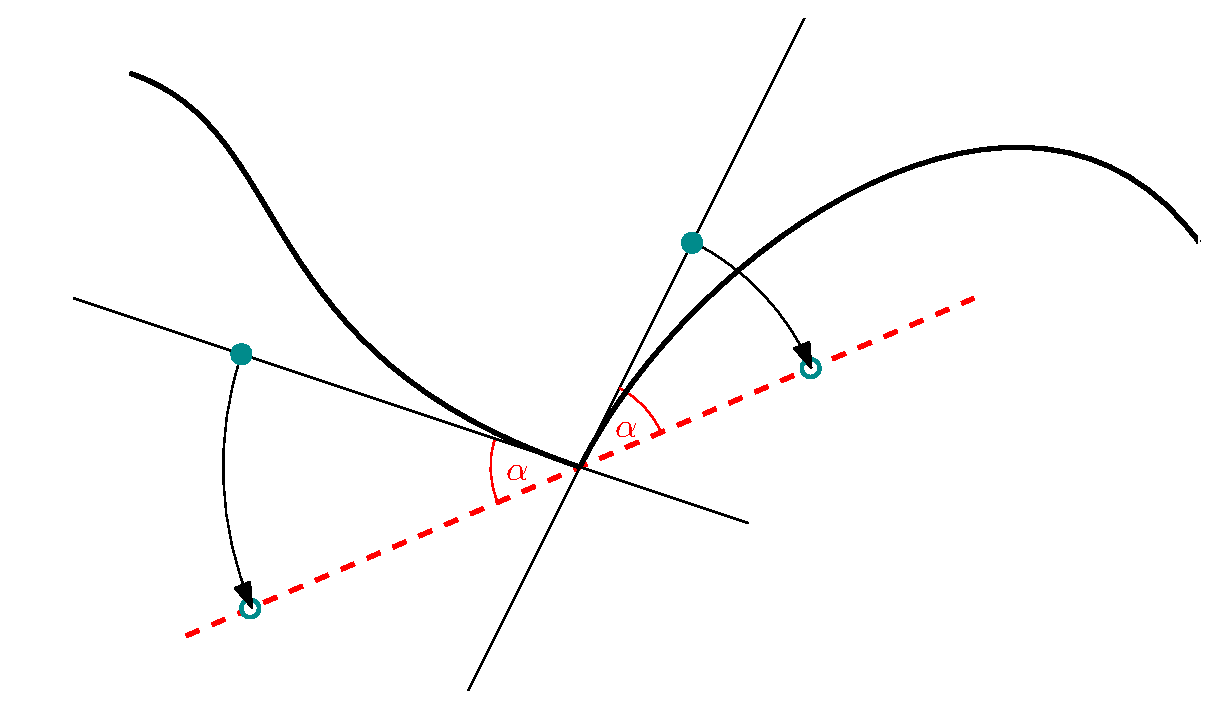
\includegraphics[width=0.5\textwidth]{graphics/smooth_spine1.eps}}
 \qquad
 \subfloat[nachher]{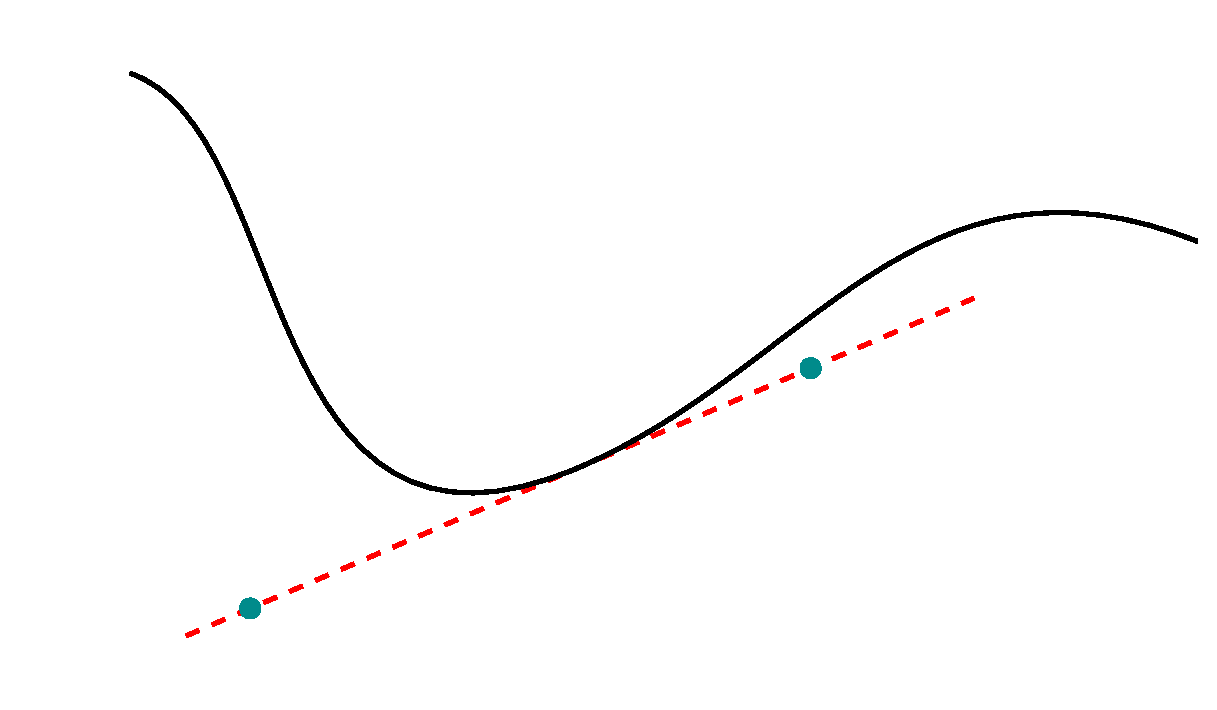
\includegraphics[width=0.5\textwidth]{graphics/smooth_spine2.eps}}
 \caption{Anpassung der Kontrollpunkte der Wirbelsäulenteile, wenn die Steigung an den Kontakpunkten ungleich ist. Die beiden Teile der Wirbelsäule und die Steigung am Kontaktpunkt sind hier in schwarz dargestellt. Die zu drehenden Kontollpunkte in cyan. In rot ist die resultierende Steigung und der Winkel, der für die Drehung verwendet wird, zu sehen.}
 \label{smooth_spine}
\end{figure}


%----------------
\section{Gelenke}

\todo{Für jede Art von Extremität und jede Position ein anderes Gelenk mit anderen Einschränkungen (nicht alle Möglichkeiten in einem)}

%----------------------------------------------------------
\section{Probleme der Beinpositionierung bei kurzen Beinen}
\label{leg_positioning_short_legs}

Wie in Absatz \ref{leg_algo} zur Ausrichtung der Beine bereits beschrieben, treten bei sehr kurzen Beinen ein paar Probleme auf. Diese werden im Folgenden kurz umrissen.

\begin{enumerate}
 \item % Bodenhöhe nicht von Gelenk aus gemessen
   Bei Berechnung der Bodenhöhe wird die Beinlänge von den entsprechenden Kontrollpunkten der Bézierkurve aus gemessen, da die Position der Hüfte/Schulter in diesem Stadium noch nicht klar ist. Deshalb kann es bei sehr kurzen Beinen sein, dass der Abstand zwischen Boden und Gelenk zu groß ist und der Boden nicht erreichbar ist.
   
   In diesem Fall wird das Bein einfach komplett ausgestreckt senkrecht nach unten positioniert. Da der Abstand zwischen dem Hüft- / Schultergelenk und dem Kontrollpunkt der Bézierkurve nicht sehr groß ist, ist auch der Abstand zu Bodenhöhe nicht enorm und fällt nicht allzusehr auf.
   
 \item % keine starke Änderung durch Drehung der Gelenke
   Bei sehr kurzen Knochen ändert sich der Abstand zum Boden durch Drehung der Gelenke nicht so stark wie bei langen Knochen. Wenn der Winkel sich zu wenig ändert, wird aber davon ausgegangen, dass die Winkeländerung zu klein ist und alle Änderungen sofort wieder zurückgesetzt wurden. Deshalb wird die Winkeländerung dann für die nächste Iteration stärker verkleinert. Das ist aber in diesem Fall kontraproduktiv. Der Algorithmus schafft es dann nämlich nicht mehr die Knochen in die richtige Lage zu bringen, da der Bewegungsspielraum dadurch zu stark eingeschänkt wird.
   
   Dem könnte man natürlich entgegenwirken, indem man, statt die Änderung des Abstandes zum Boden zu messen, abfragt wie oft die Drehungen in der jeweiligen Iteration zurückgesetzt wurden.
   
 \item % ganz kurze Beine
   Bei wirklich sehr kurzen Beinen (hier eine Gesamtlänge unter 5) macht es gar keinen Sinn sie anzuordnen, da man sie kaum sieht. Außerdem tritt hier der Effekt auf, der in Punkt 2 schon beschrieben wurde.
   
 \item % Beinstartpos unter Bodenhöhe
   Die Beinstartposition kann schon vor der ersten Iteration unterhalb der Bodenhöhe liegen. Das tritt auf, wenn mindestens ein Paar Beine sehr kurz ist und die Wirbelsäule an den Ansatzpunkten auf sehr unterschiedlicher Höhe liegt (siehe auch Absatz \ref{floor_height} zur Berechnung der Bodenhöhe).
   \todo{Beispiel: Dimetrodon}
   
   In diesem Fall ist der Algorithmus natürlich nicht anwendbar. Das Bein wird dann einfach senkrecht nach unten ausgerichtet und mit einem Fuß versehen, der mit der Sohle auf dem Boden steht.
   
 \item % Gelenkoffsets
   Bei kurzen Beinknochen kann es dazu kommen, dass der Oberschenkel nicht näher zum Boden kann, weil er schon aufliegt, aber Schienbein und Hand durch das Gelenkoffset (siehe Kapitel \ref{chapter:bone_models} zur Positionierung der Knochenmodelle) über dem Boden schweben und nicht näher zum Boden bewegt werden können.
   \todo{Beispiel Krokodil (siehe auch Screenshot)}
\end{enumerate}











%% --------------------
%% |   Bibliography   |
%% --------------------

%% Add entry to the table of contents for the bibliography
\printbibliography[heading=bibintoc]

%% ----------------
%% |   Appendix   |
%% ----------------
\begin{appendices}
%-------------------------------
%-------------------------------
\chapter{PCA Daten}
\label{appendix_pca}

%-----------------------------
\section{Eingabedaten für PCA}

%- - - - - - - - - 
\subsection{Bilder}
\label{picture_sources}
 
 Alle Bilder, die als Eingabe für die PCA verwendet wurden, sind in Abbildung \ref{all_images} zu finden. Im Folgenden sind die Bildquellen aufgezählt.
 Alle Tiere, die nicht aufgezählt sind, sind aus \cite{Spezielle_Zoologie} entnommen.
 \begin{itemize}
  \item Archaeopteryx, Ichthyosaurus, Ichthyostega, Urpferdchen aus \cite{Zoologie24Wehner}
  \item Blauwal \url{https://www.quagga-illustrations.de/wp-content/uploads/2014/05/h0001705.jpg}
  \item Chamäleon \url{https://www.madcham.de/de/anatomie/}
  \item Dormedar \url{https://upload.wikimedia.org/wikipedia/commons/a/ac/Camel_Skeleton_-_Richard_Owen_-_On_the_Anatomy_of_Vertebrates_\%281866\%29.jpg}
  \item Giraffe\\ \url{https://de.wikipedia.org/wiki/Giraffen#/media/Datei:Giraffe_skeleton.jpg}
  \item Gnu \url{https://lutzmoeller.net/Afrika/2007/Lutz-Juli/8-Gnu.php}
  \item Känguru \url{http://www.bildwoerterbuch.com/tierreich/beuteltiere/kaenguru/skelett-eines-kaengurus.php}
  \item Krokodil \url{https://de.depositphotos.com/210906852/stock-illustration-skeleton-crocodile-vintage-line-drawing.html}
  \item Pferd \url{https://www.kosmos.de/content/buecher/ratgeber/pferde-reiten/vorwaerts-abwaerts-eine-frage-der-haltung/}
  \item Schlange: zu Schlangen gibt es keine Bilder, die deren Skelett in ausgestrecktem Zustand von der Seite darstellen. Deshalb wurde ein leeres Bild genommen und der Verlauf des Rückens durch eine Gerade angenähert (Extremitäten besitzt eine Schlange nicht. Außerdem ist nicht erkennbar ob \bzw wo Hals in Rücken und Rücken in Schwanz übergeht. Deshalb wurde die komplette Wirbelsäule als Rücken markiert.)
  \item Schwan \url{https://www.alamy.de/skelett-eines-schwans-osteographia-oder-die-anatomie-der-knochen-london-1733-quelle-47-ich-12-kapitel-v-saitenhalter-autor-cheselden-william-image226921369.html}
  \item Sinornis und Taube aus \cite{Vergleichende_Anatomie}
  \item Strauß \url{https://www.alamy.de/stockfoto-skelett-von-strauss-24658845.html}
  \item Tyrannosaurus Rex \url{https://upload.wikimedia.org/wikipedia/commons/9/9f/Tyrannosaurus_skeleton.jpg}
 \end{itemize}
 
\begin{figure}
\subfloat[Afrikanischer Elefant]{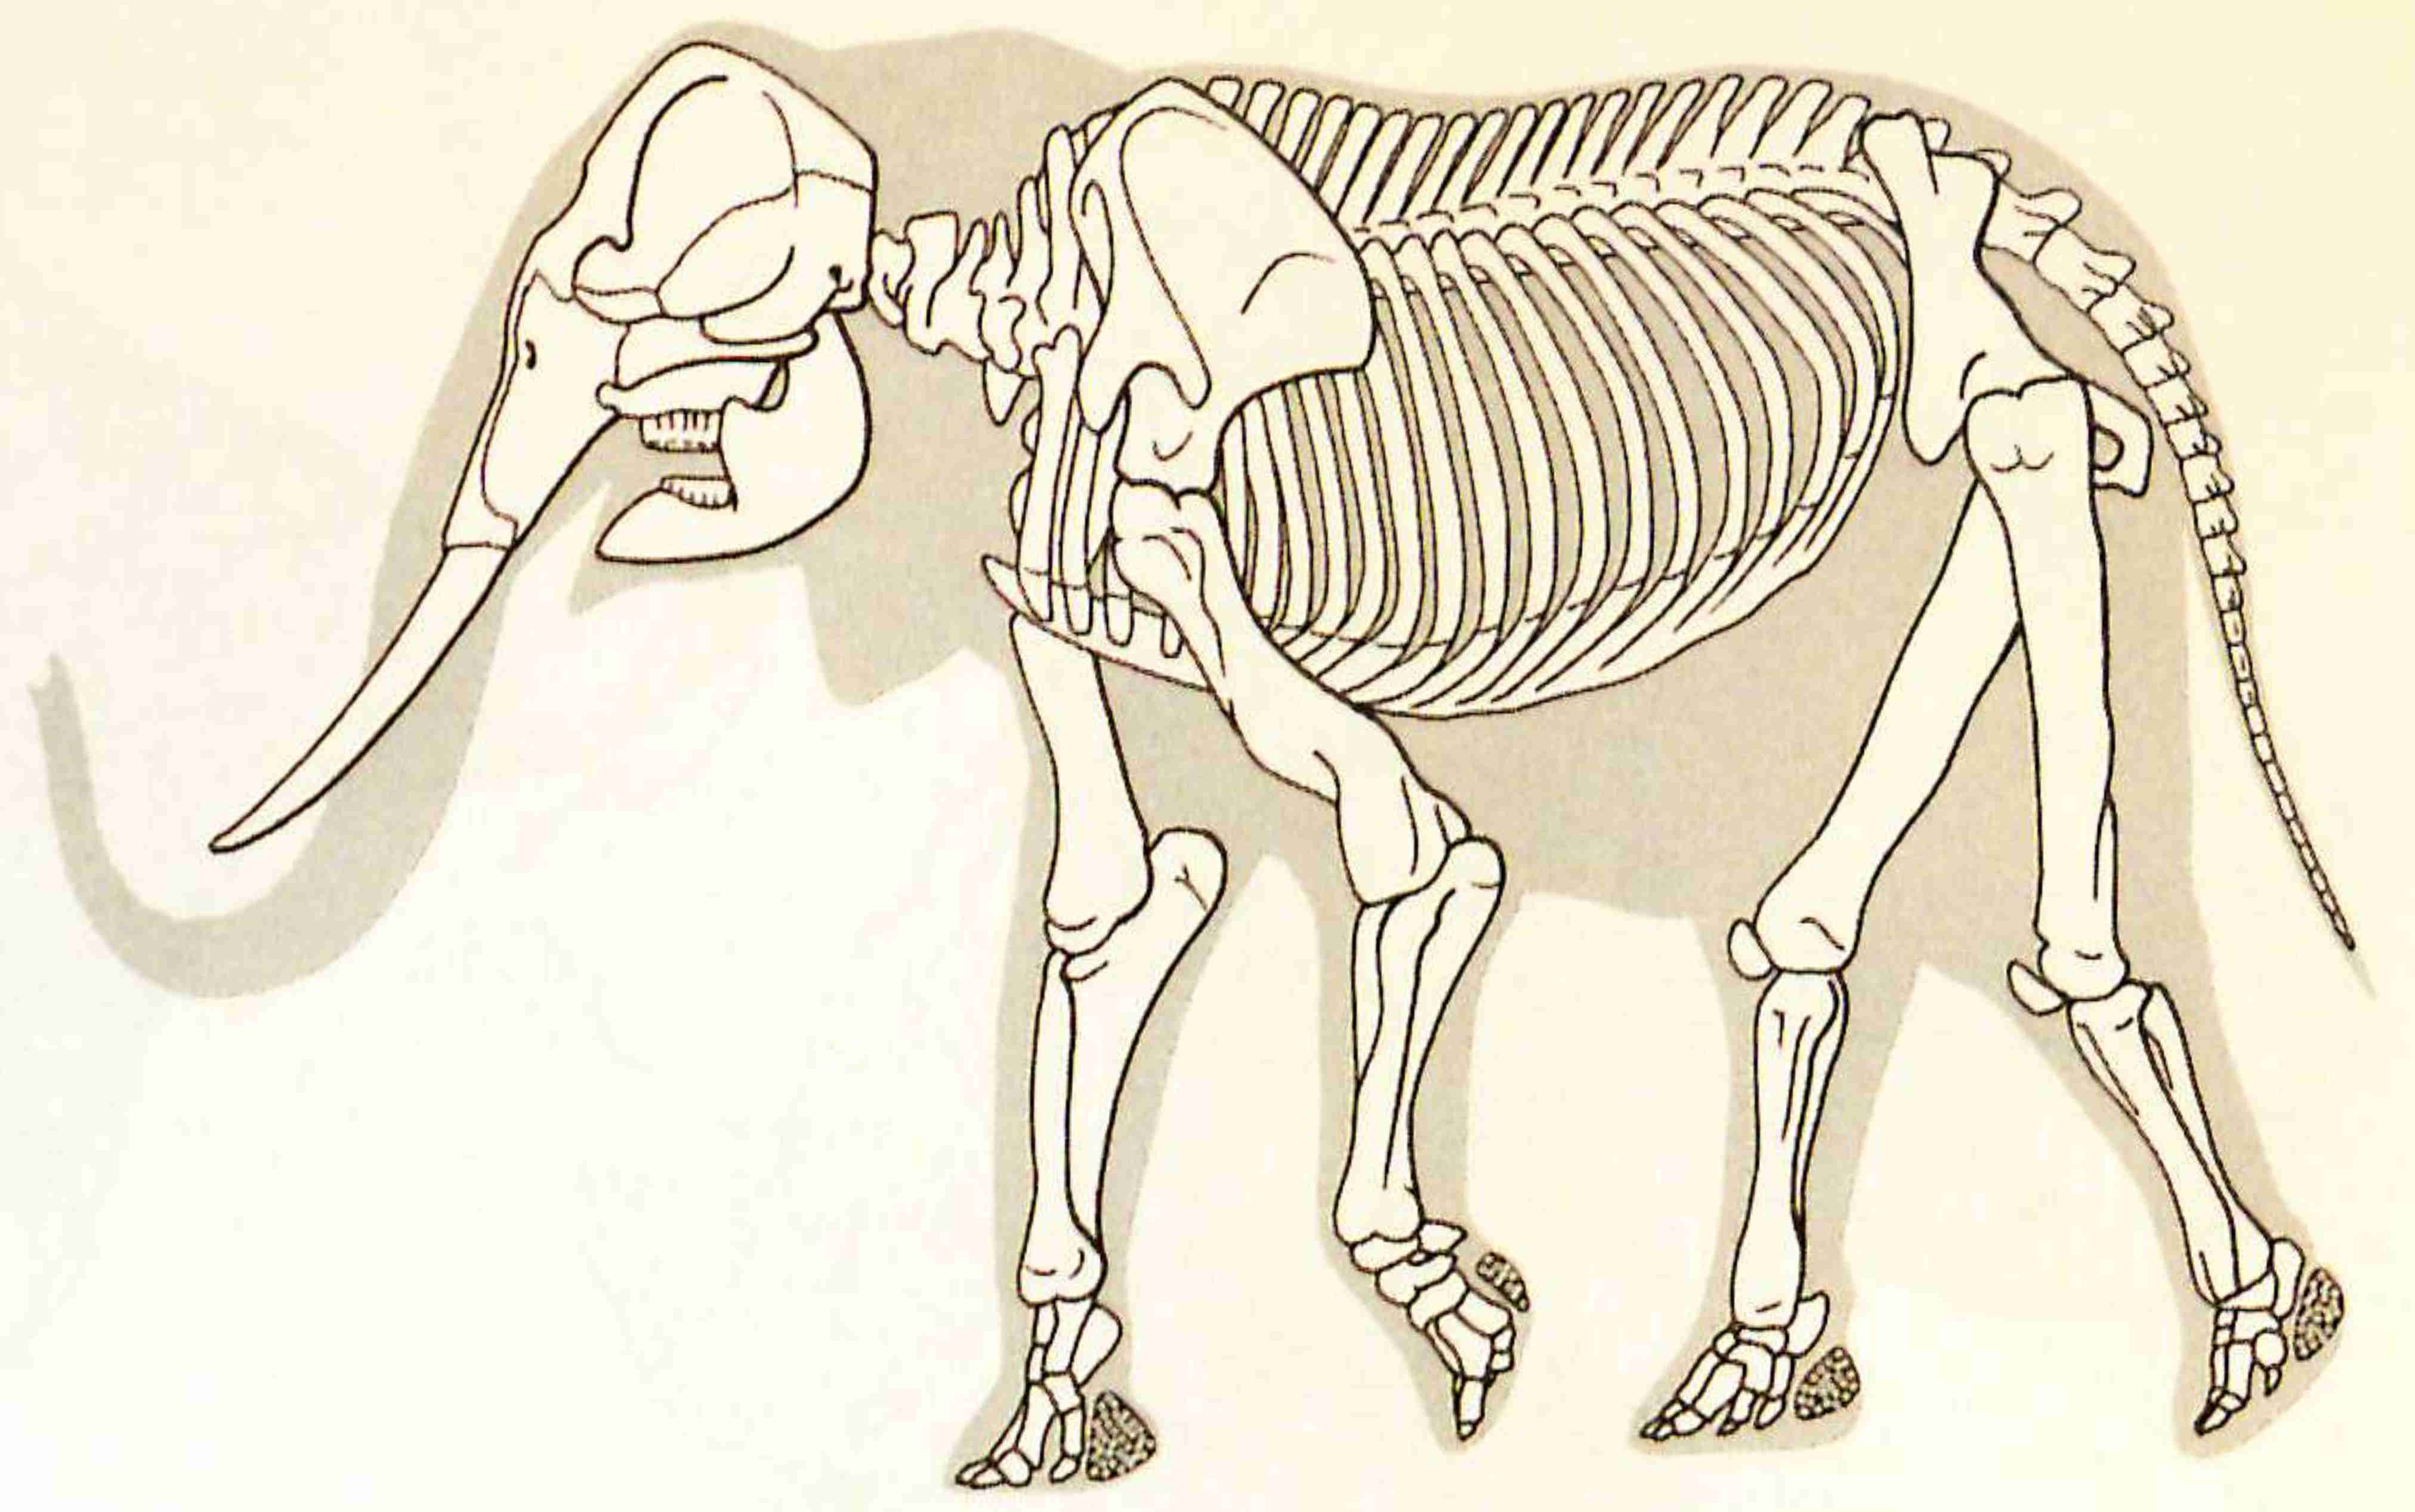
\includegraphics[width=0.2\textwidth]{../PCA/Skelettbilder_klein/Afrikanischer_Elefant.jpg}}~
\subfloat[Amerikanischer Flussbarsch]{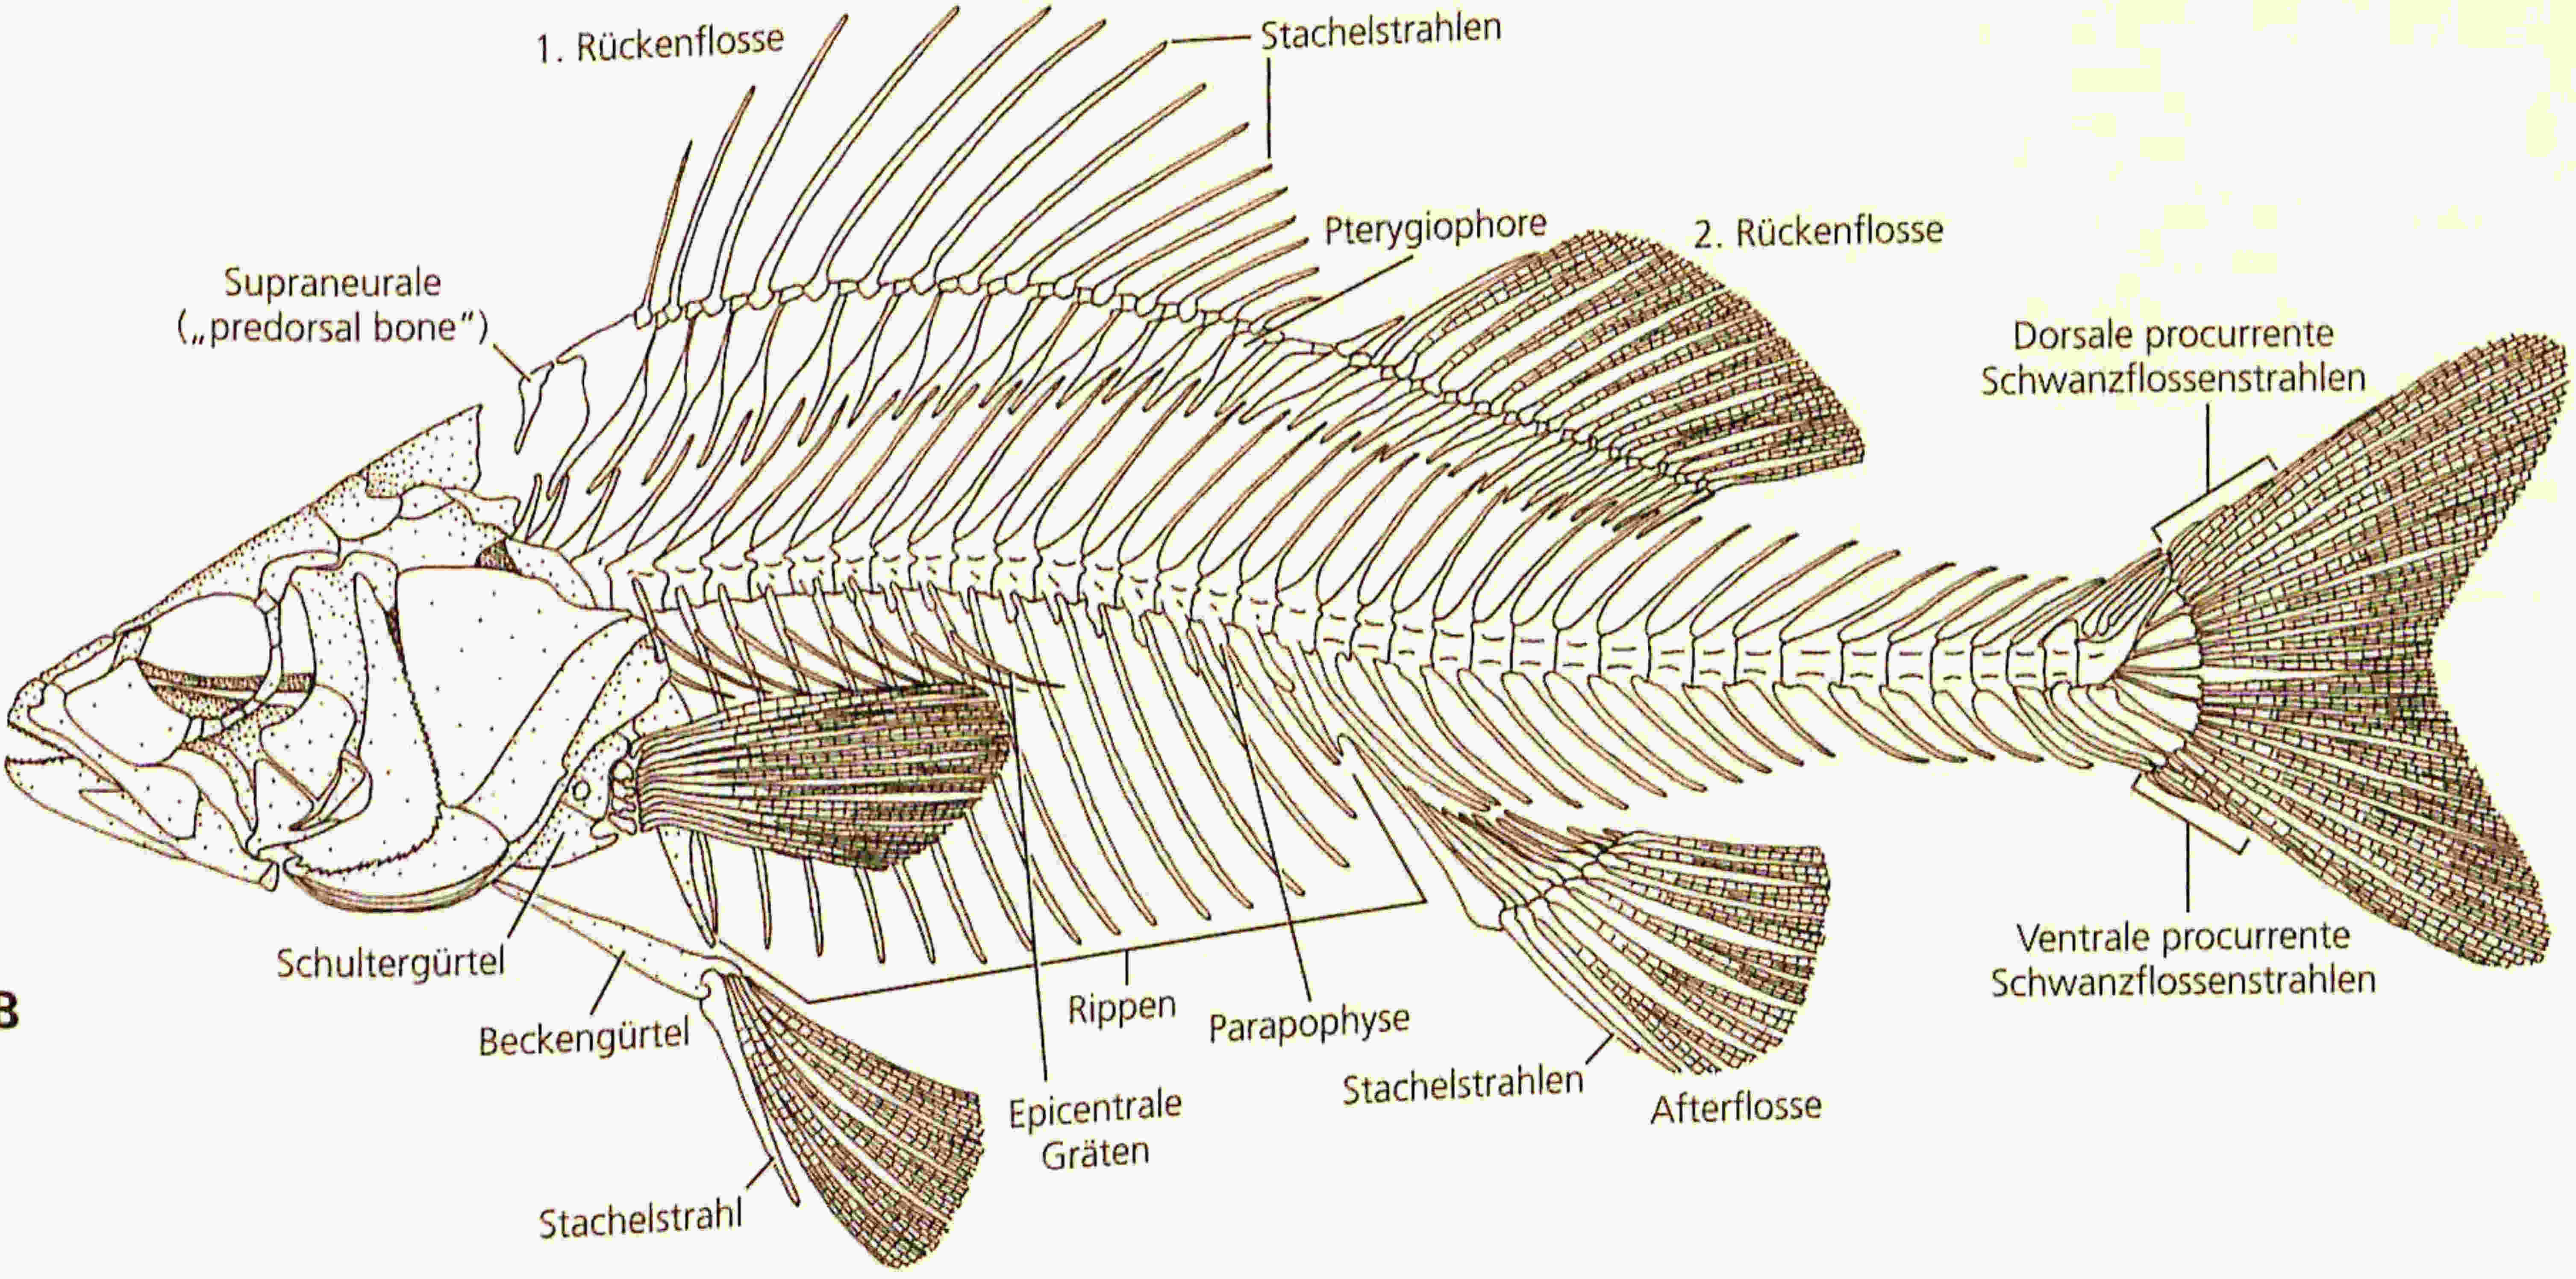
\includegraphics[width=0.2\textwidth]{../PCA/Skelettbilder_klein/Amerikanischer_Flussbarsch.jpg}}~
\subfloat[Archaeopteryx]{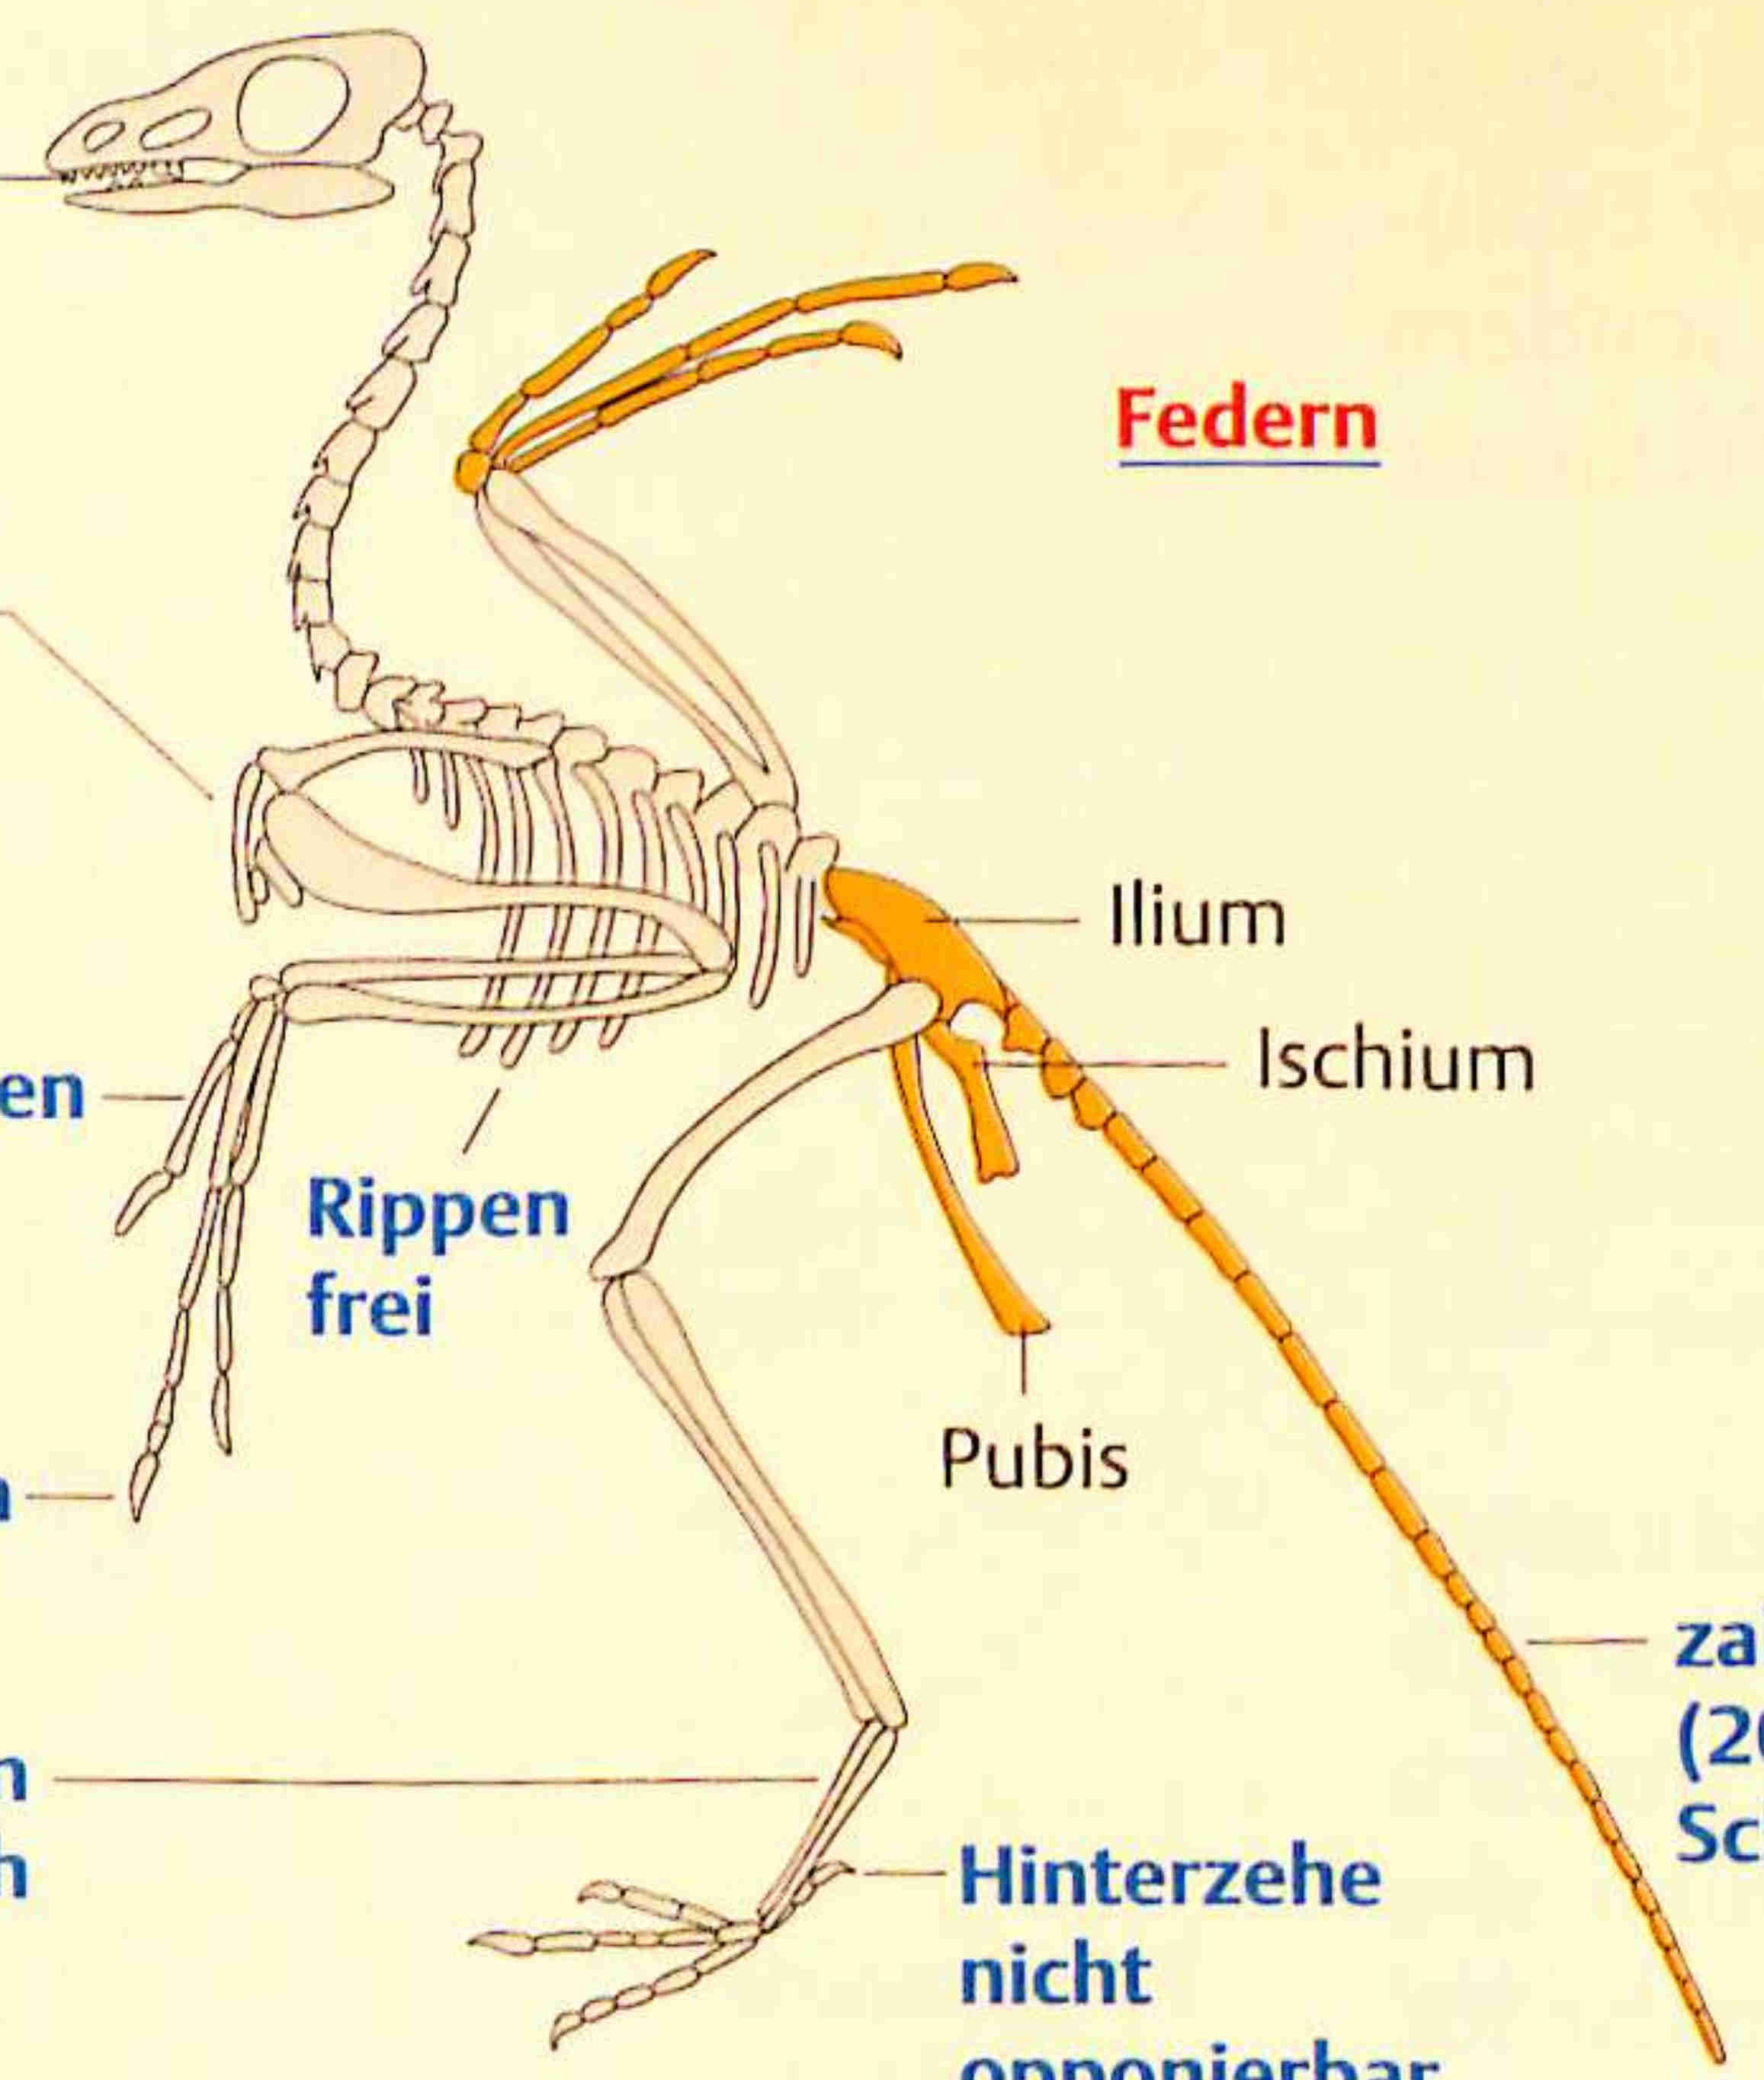
\includegraphics[width=0.2\textwidth]{../PCA/Skelettbilder_klein/Archaeopteryx.jpg}}~
\subfloat[Blauwal]{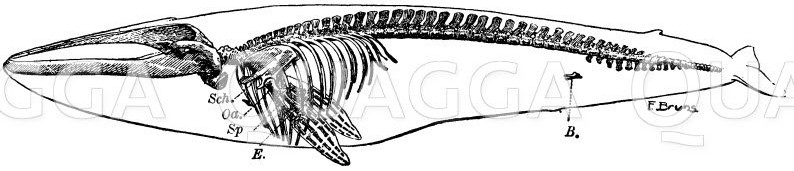
\includegraphics[width=0.2\textwidth]{../PCA/Skelettbilder_klein/Blauwal.jpg}}~
\subfloat[Brachiosaurus]{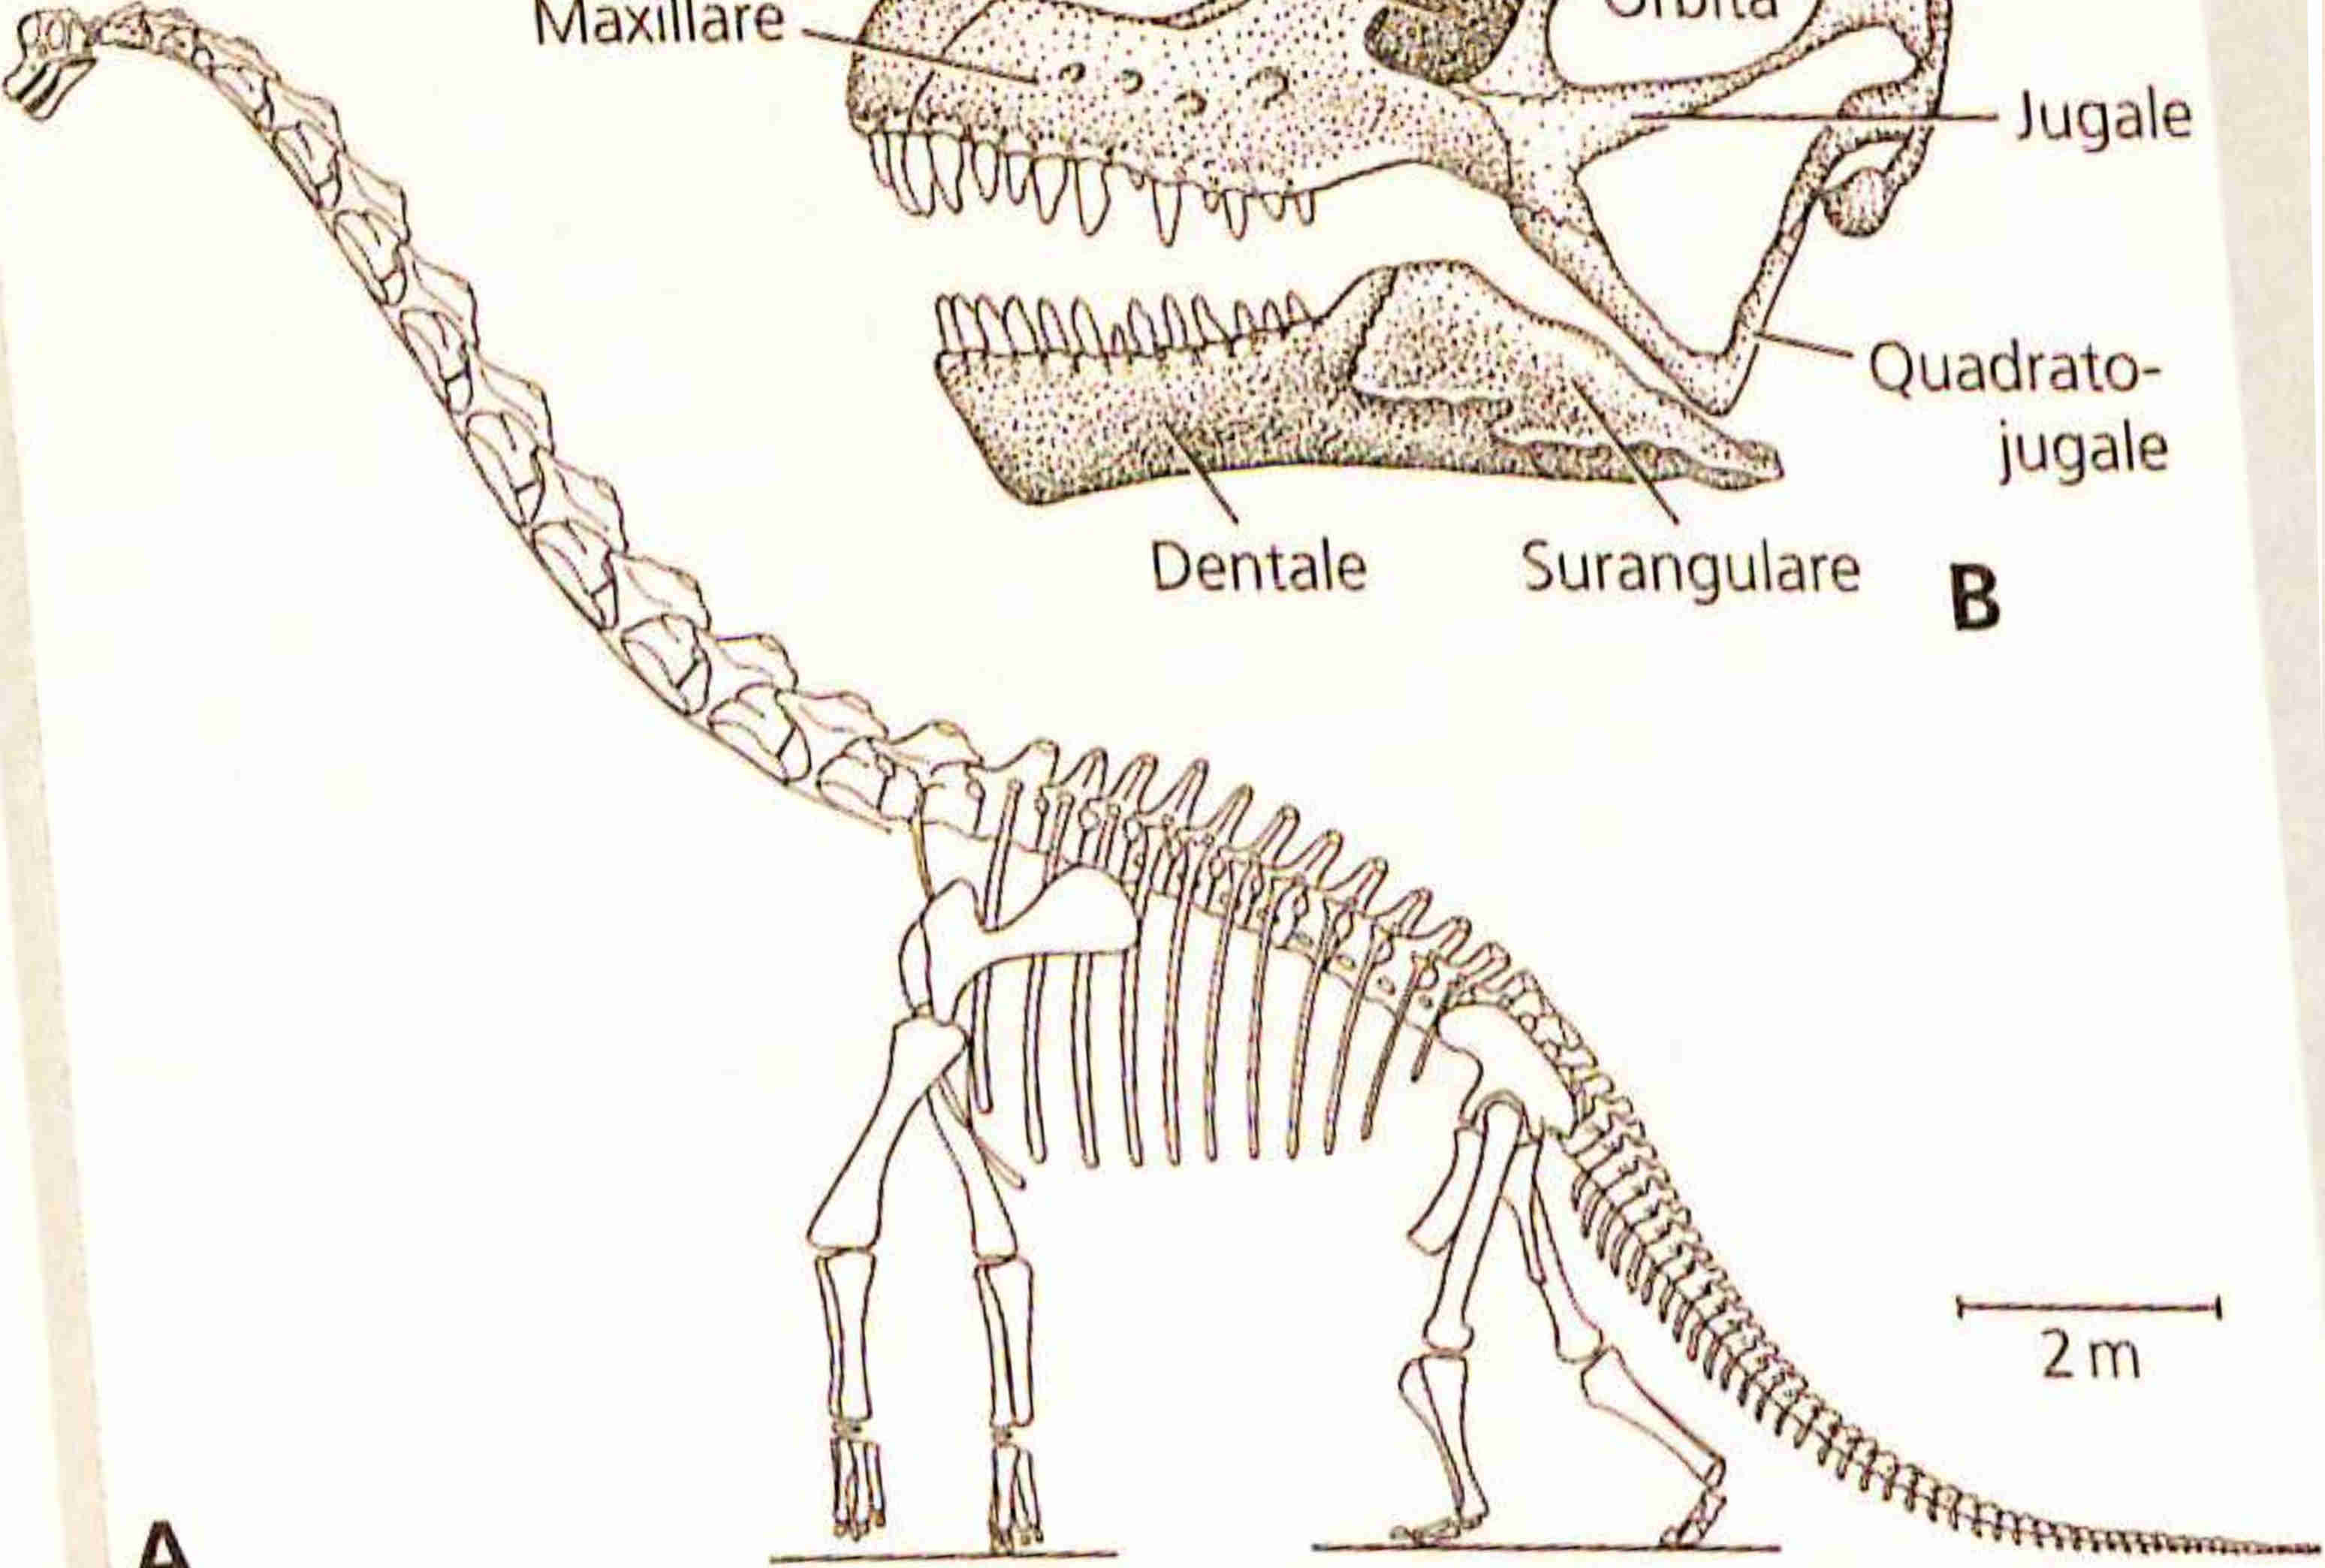
\includegraphics[width=0.2\textwidth]{../PCA/Skelettbilder_klein/Brachiosaurus.jpg}}
\\
\subfloat[Chamäleon]{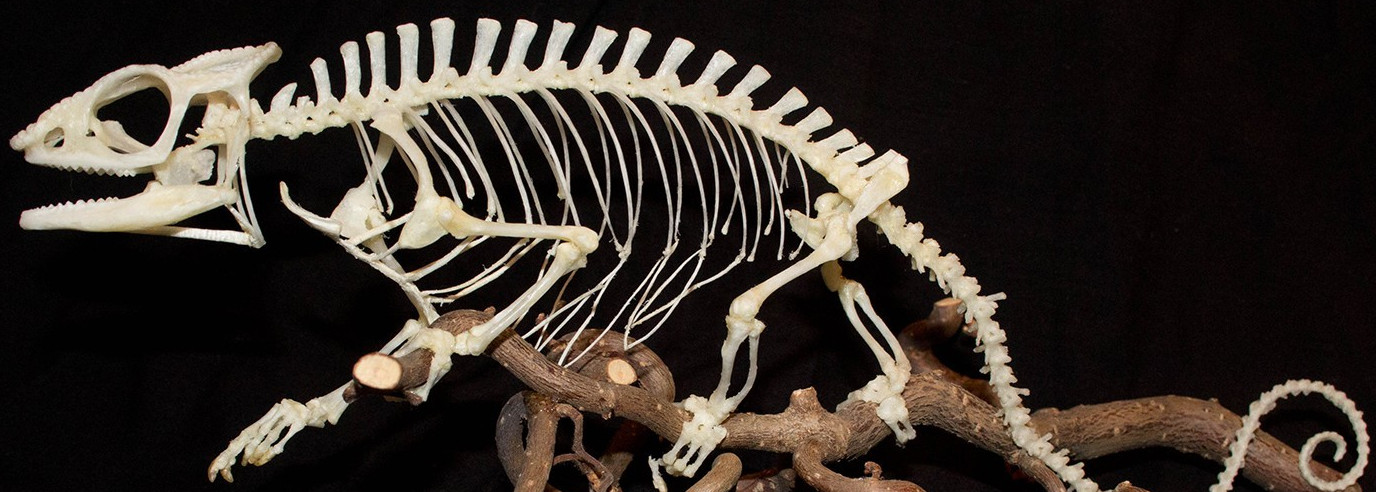
\includegraphics[width=0.2\textwidth]{../PCA/Skelettbilder_klein/Chamaeleon.jpg}}~
\subfloat[Dimetrodon]{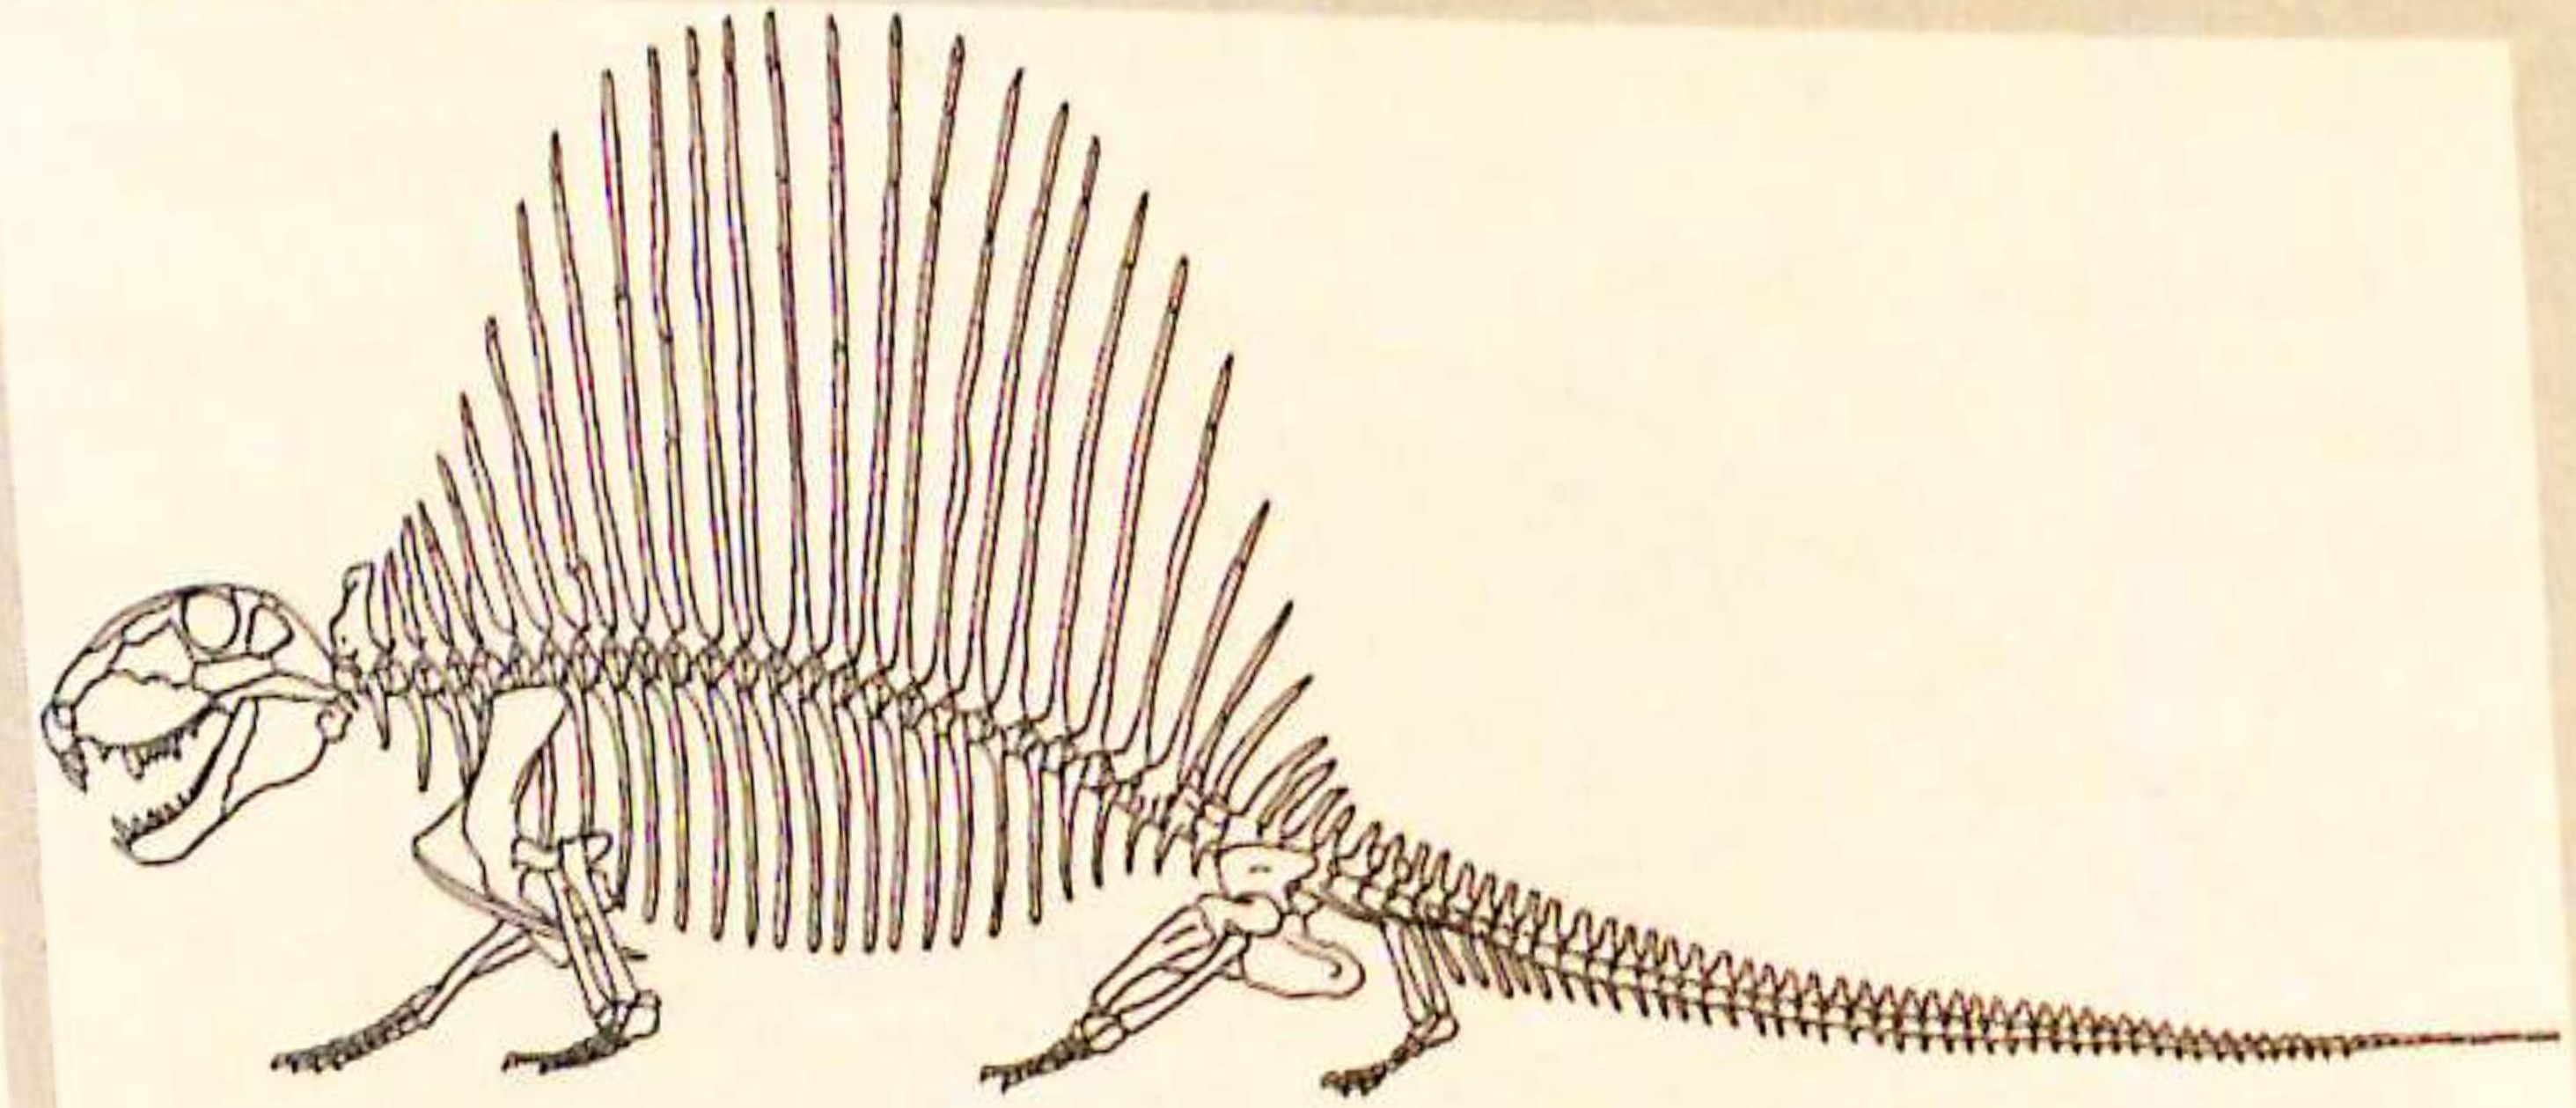
\includegraphics[width=0.2\textwidth]{../PCA/Skelettbilder_klein/Dimetrodon.jpg}}~
\subfloat[Dromedar]{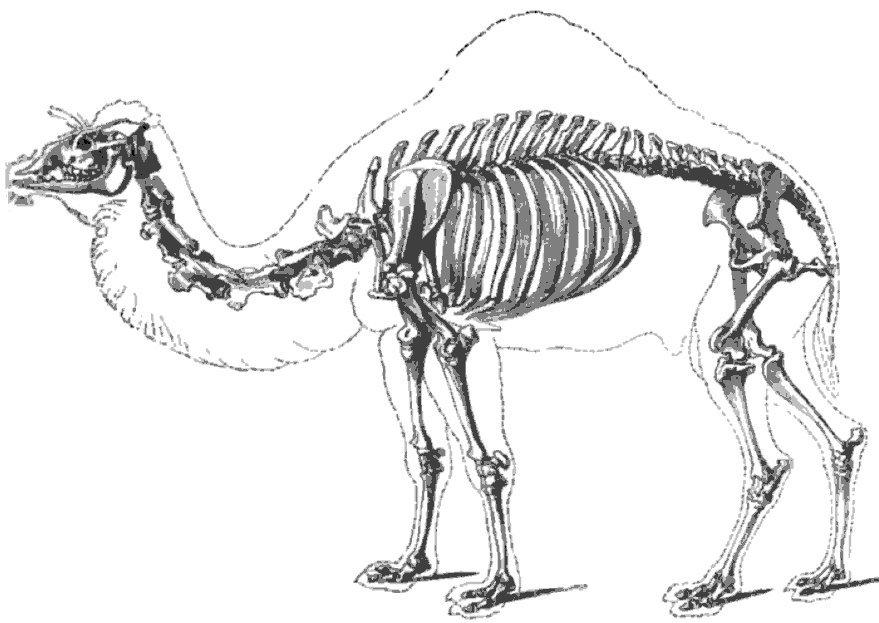
\includegraphics[width=0.2\textwidth]{../PCA/Skelettbilder_klein/Dromedar.jpg}}~
\subfloat[Elster]{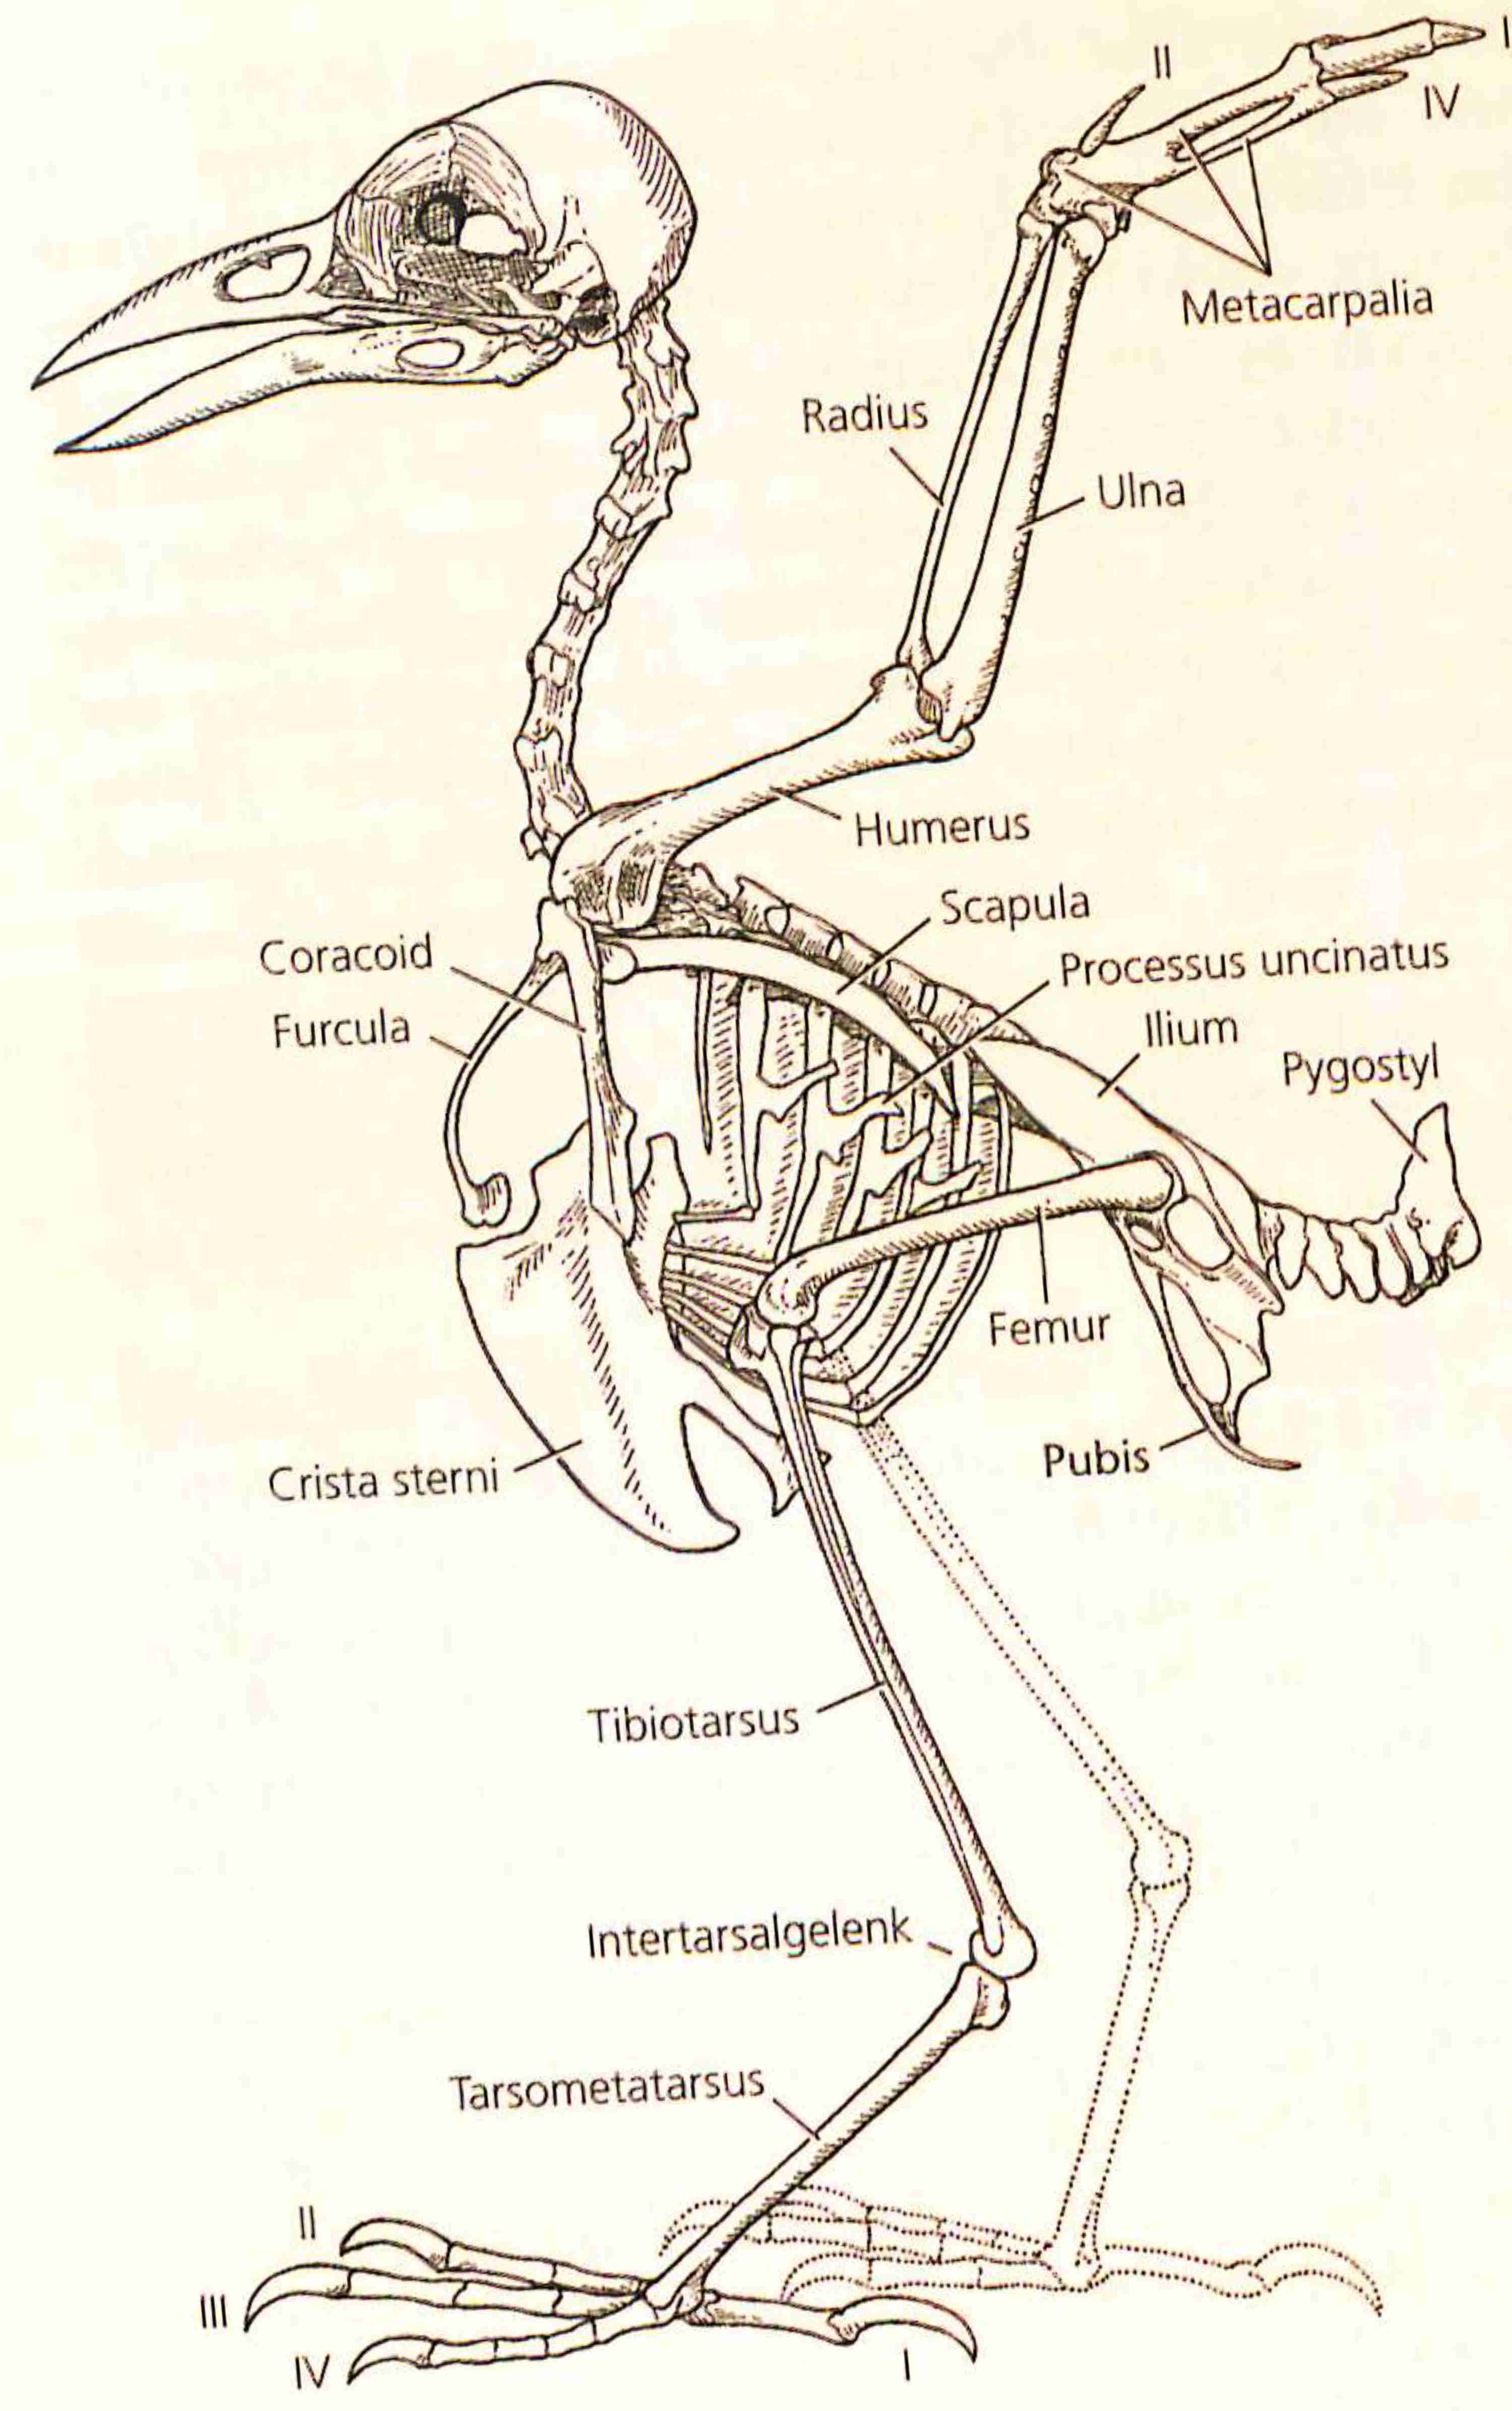
\includegraphics[width=0.2\textwidth]{../PCA/Skelettbilder_klein/Elster.jpg}}~
\subfloat[Forelle]{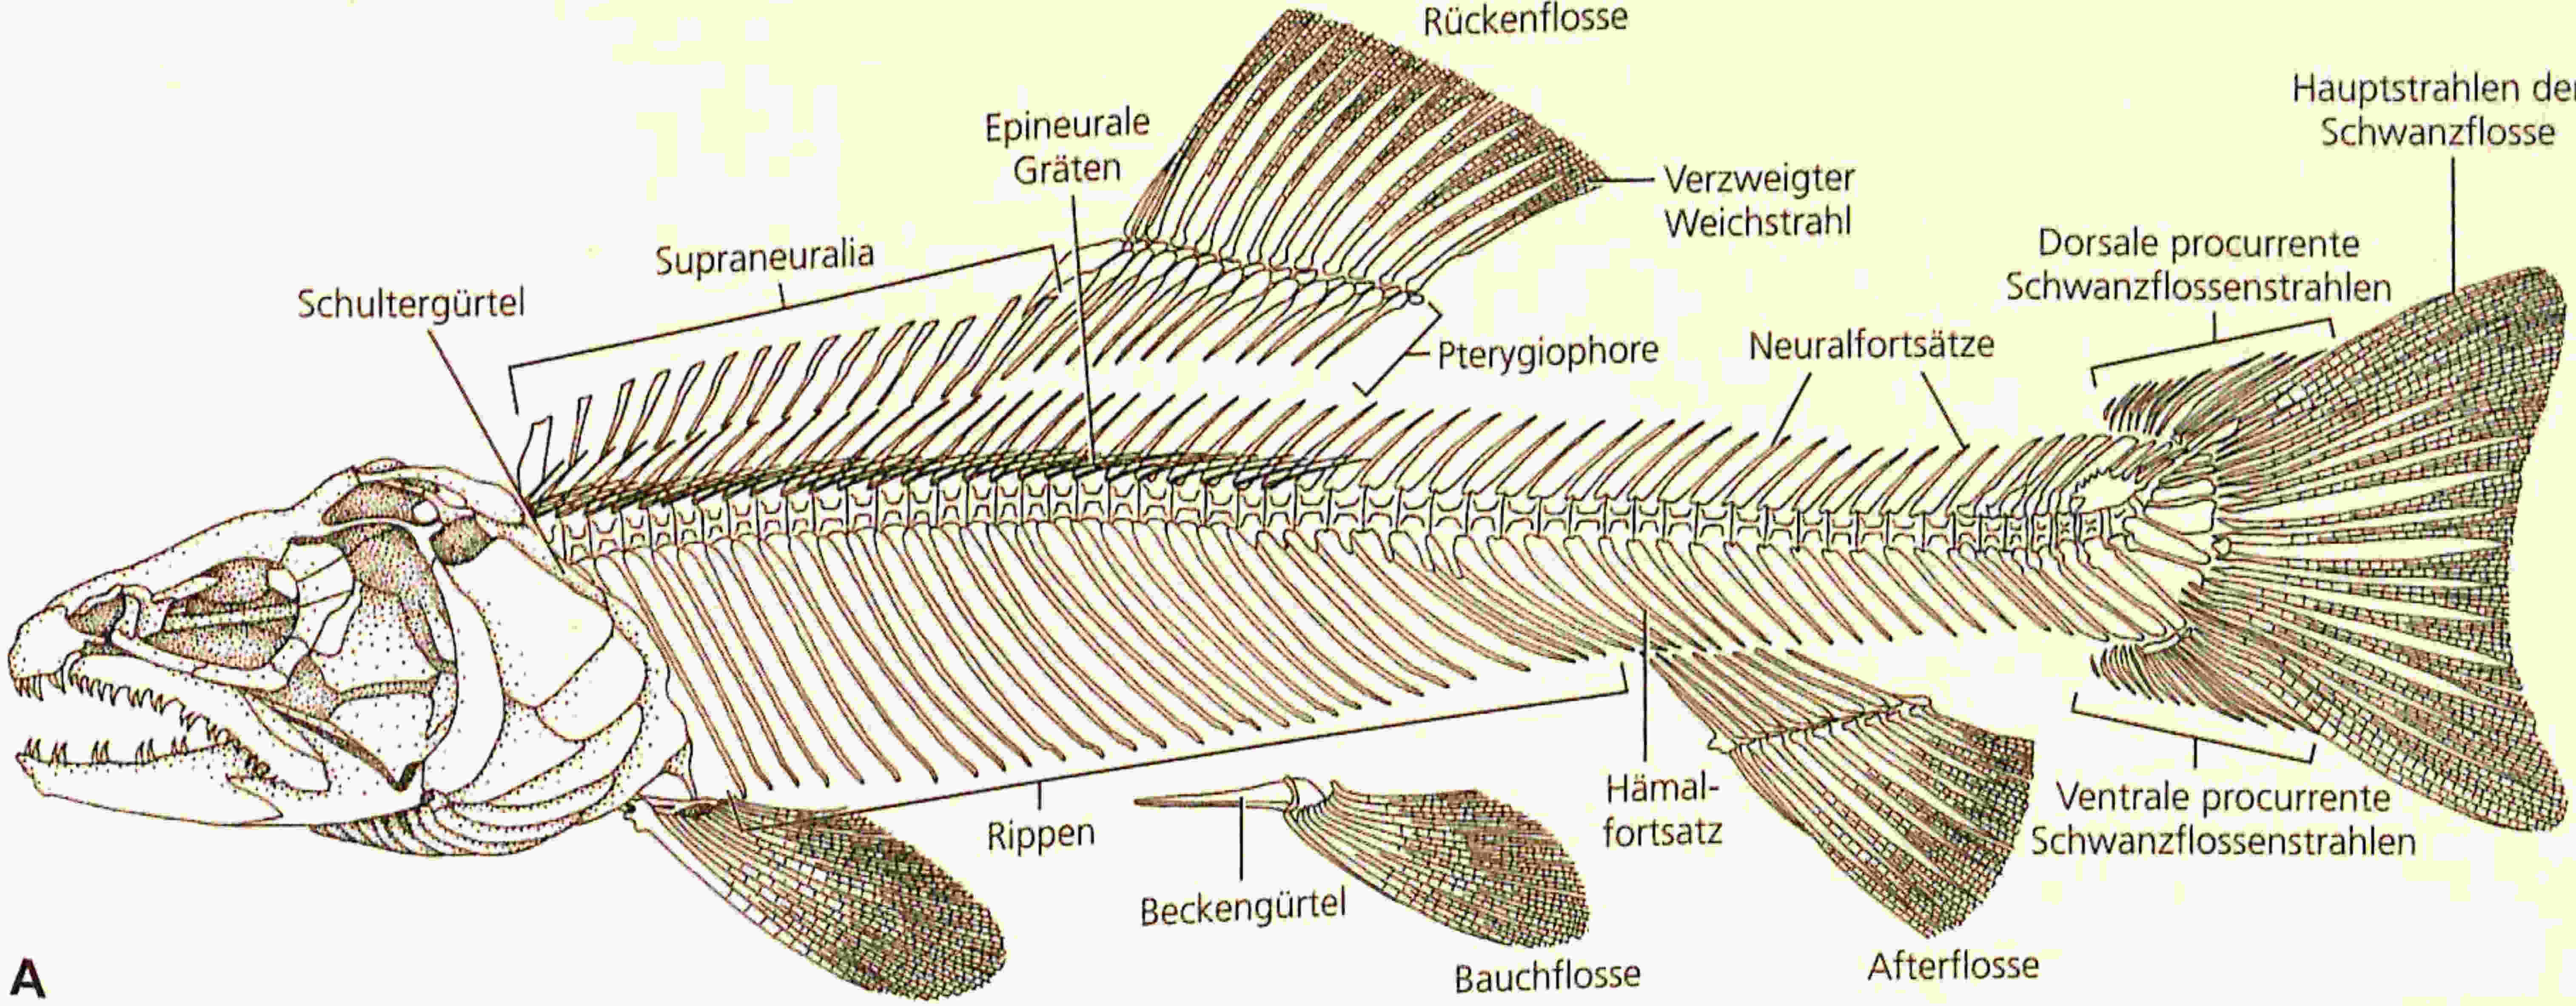
\includegraphics[width=0.2\textwidth]{../PCA/Skelettbilder_klein/Forelle.jpg}}
\\
\subfloat[Frosch]{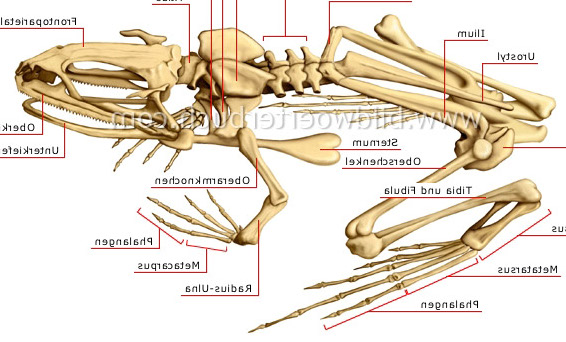
\includegraphics[width=0.2\textwidth]{../PCA/Skelettbilder_klein/Frosch.jpg}}~
\subfloat[Gämse]{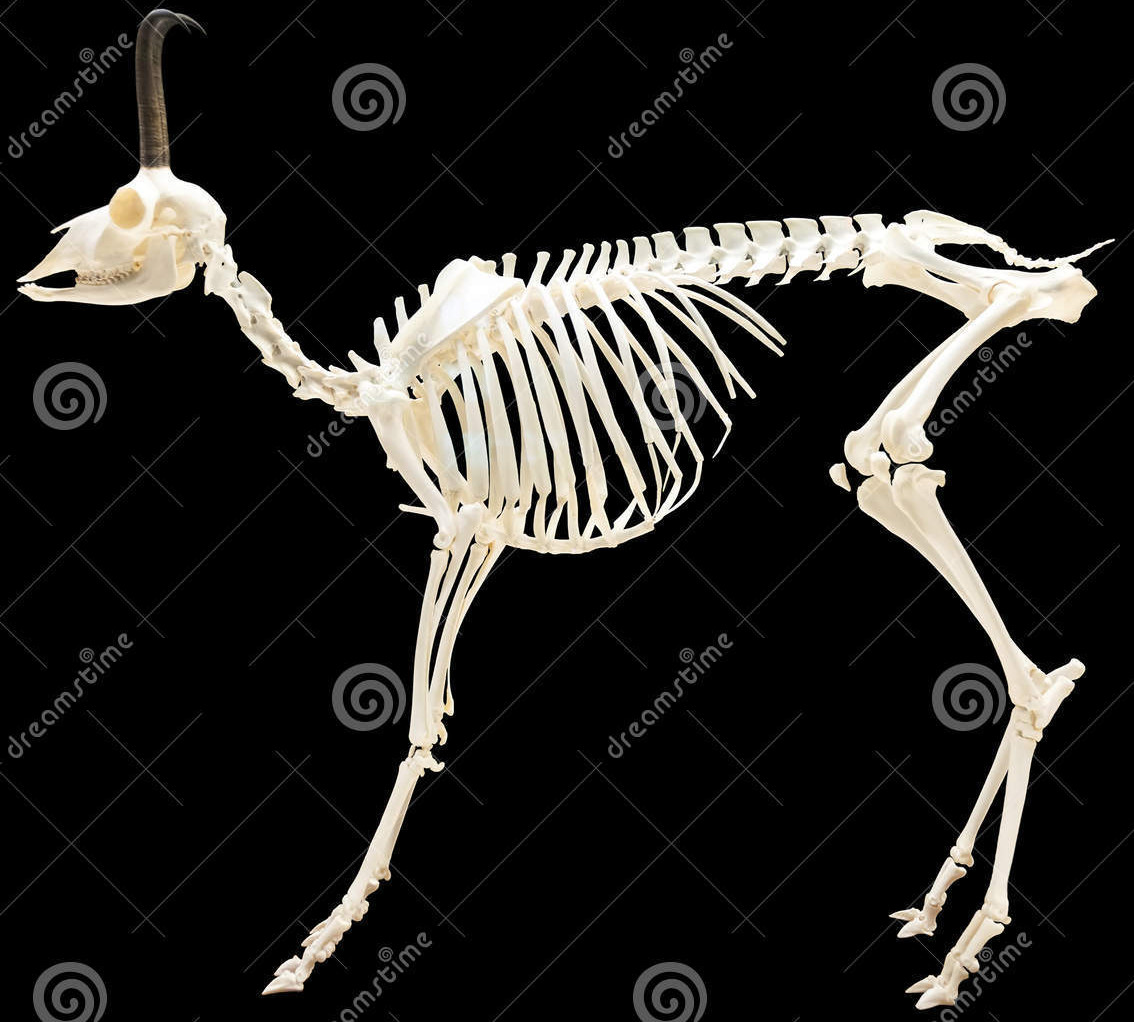
\includegraphics[width=0.2\textwidth]{../PCA/Skelettbilder_klein/Gaemse.jpg}}~
\subfloat[Giraffe]{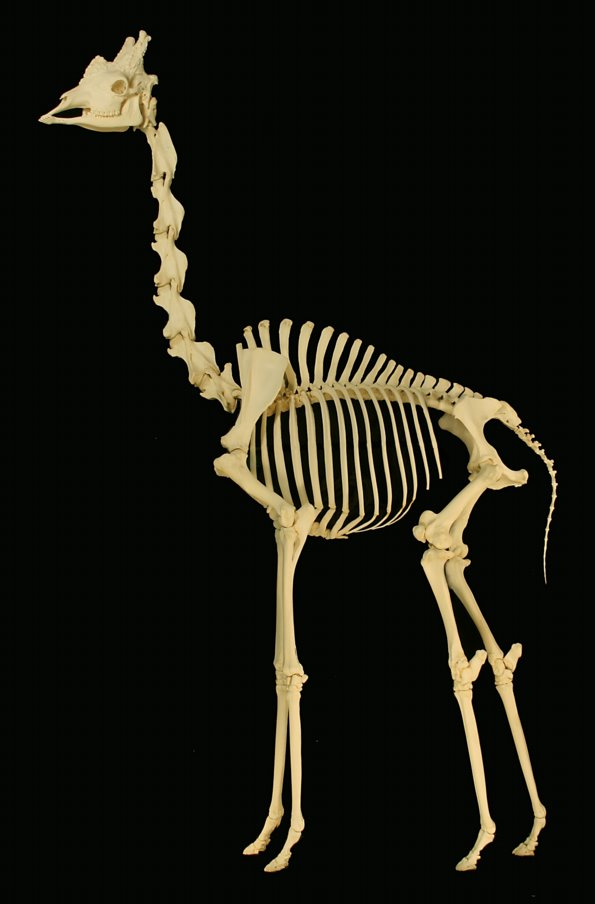
\includegraphics[width=0.2\textwidth]{../PCA/Skelettbilder_klein/Giraffe.jpg}}~
\subfloat[Gnu]{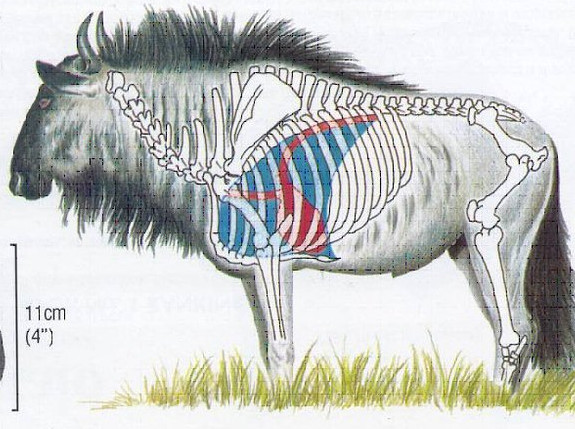
\includegraphics[width=0.2\textwidth]{../PCA/Skelettbilder_klein/Gnu.jpg}}~
\subfloat[Grönlandwal]{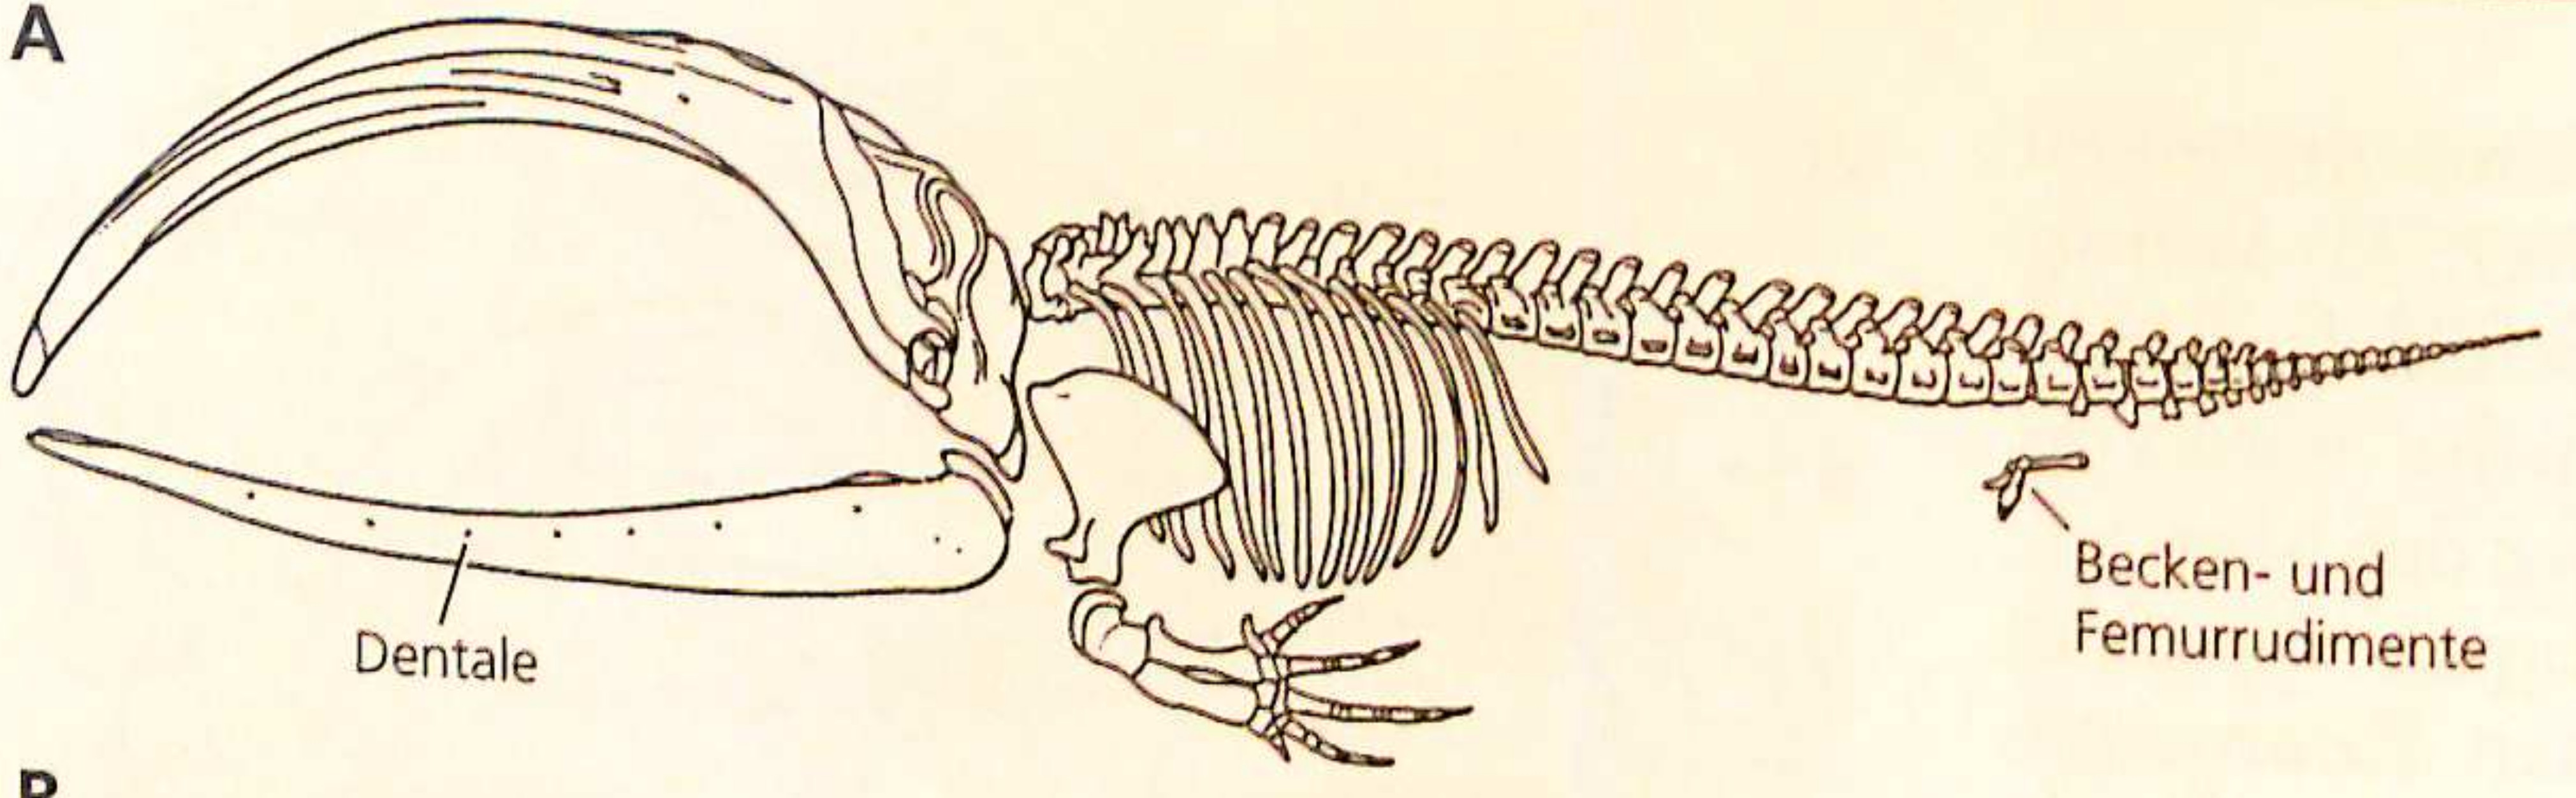
\includegraphics[width=0.2\textwidth]{../PCA/Skelettbilder_klein/Groenlandwal.jpg}}
\\
\subfloat[Ichthyornis]{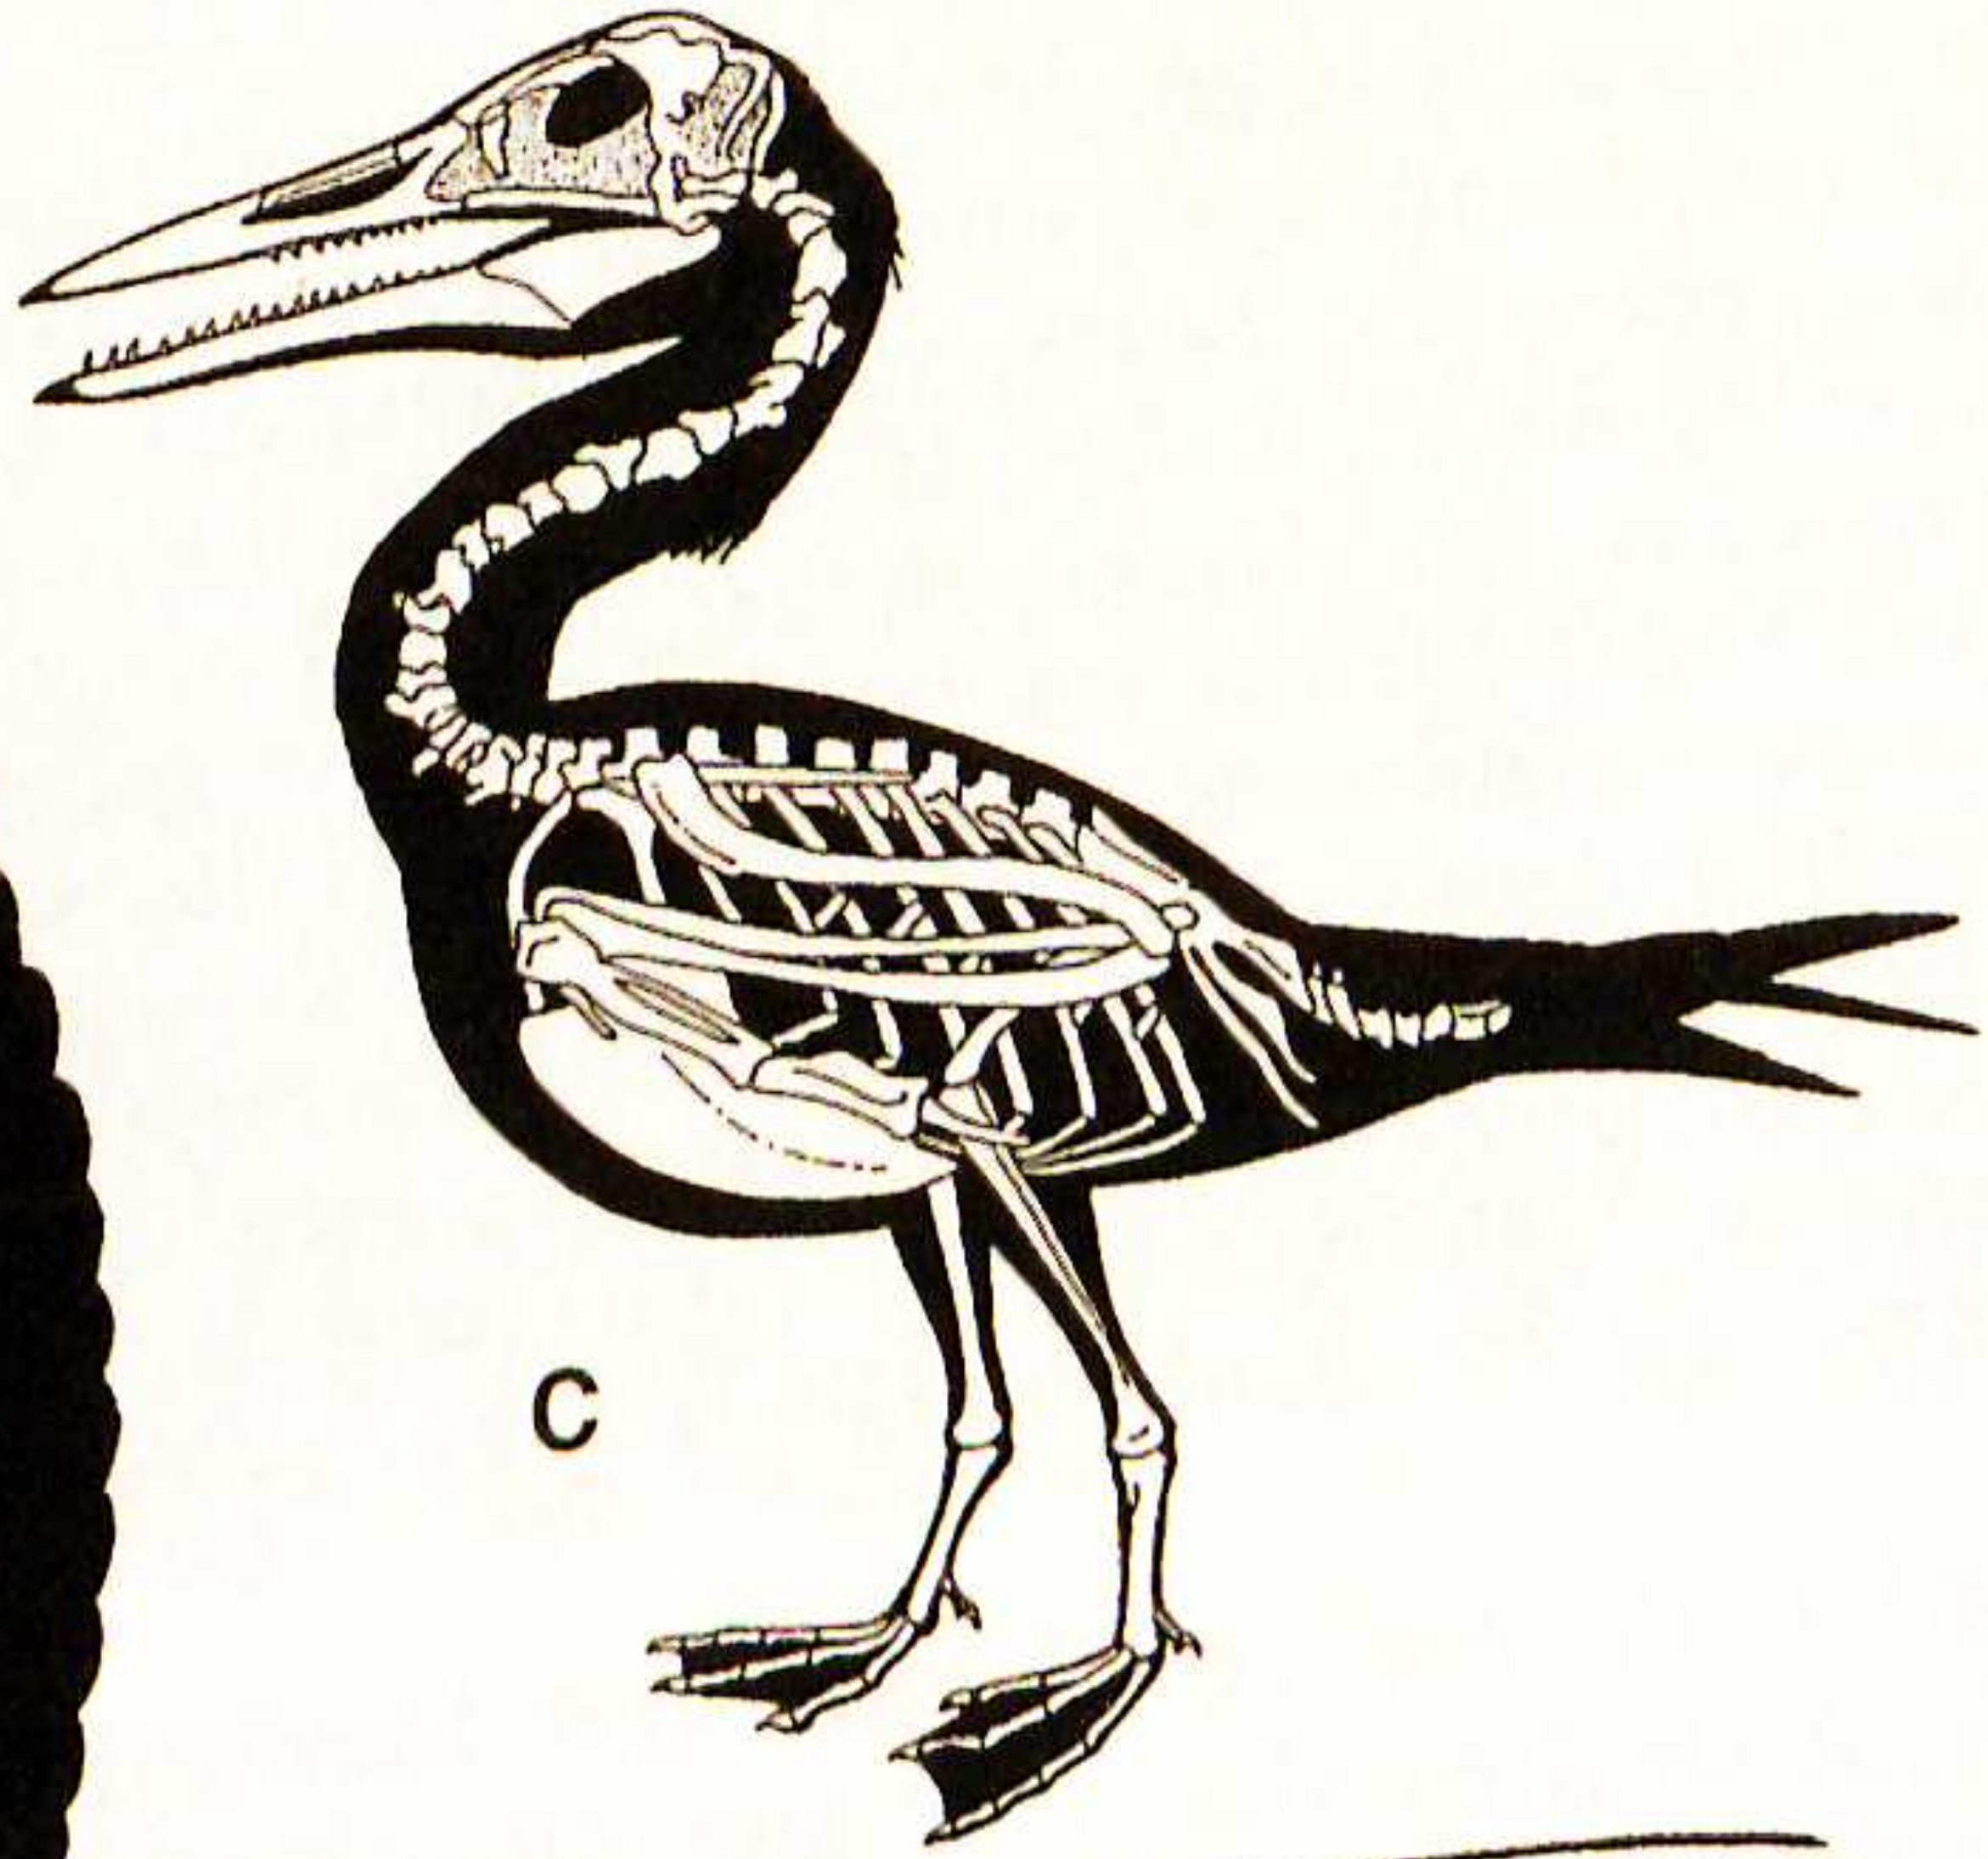
\includegraphics[width=0.2\textwidth]{../PCA/Skelettbilder_klein/Ichthyornis.jpg}}~
\subfloat[Ichthyosaurus]{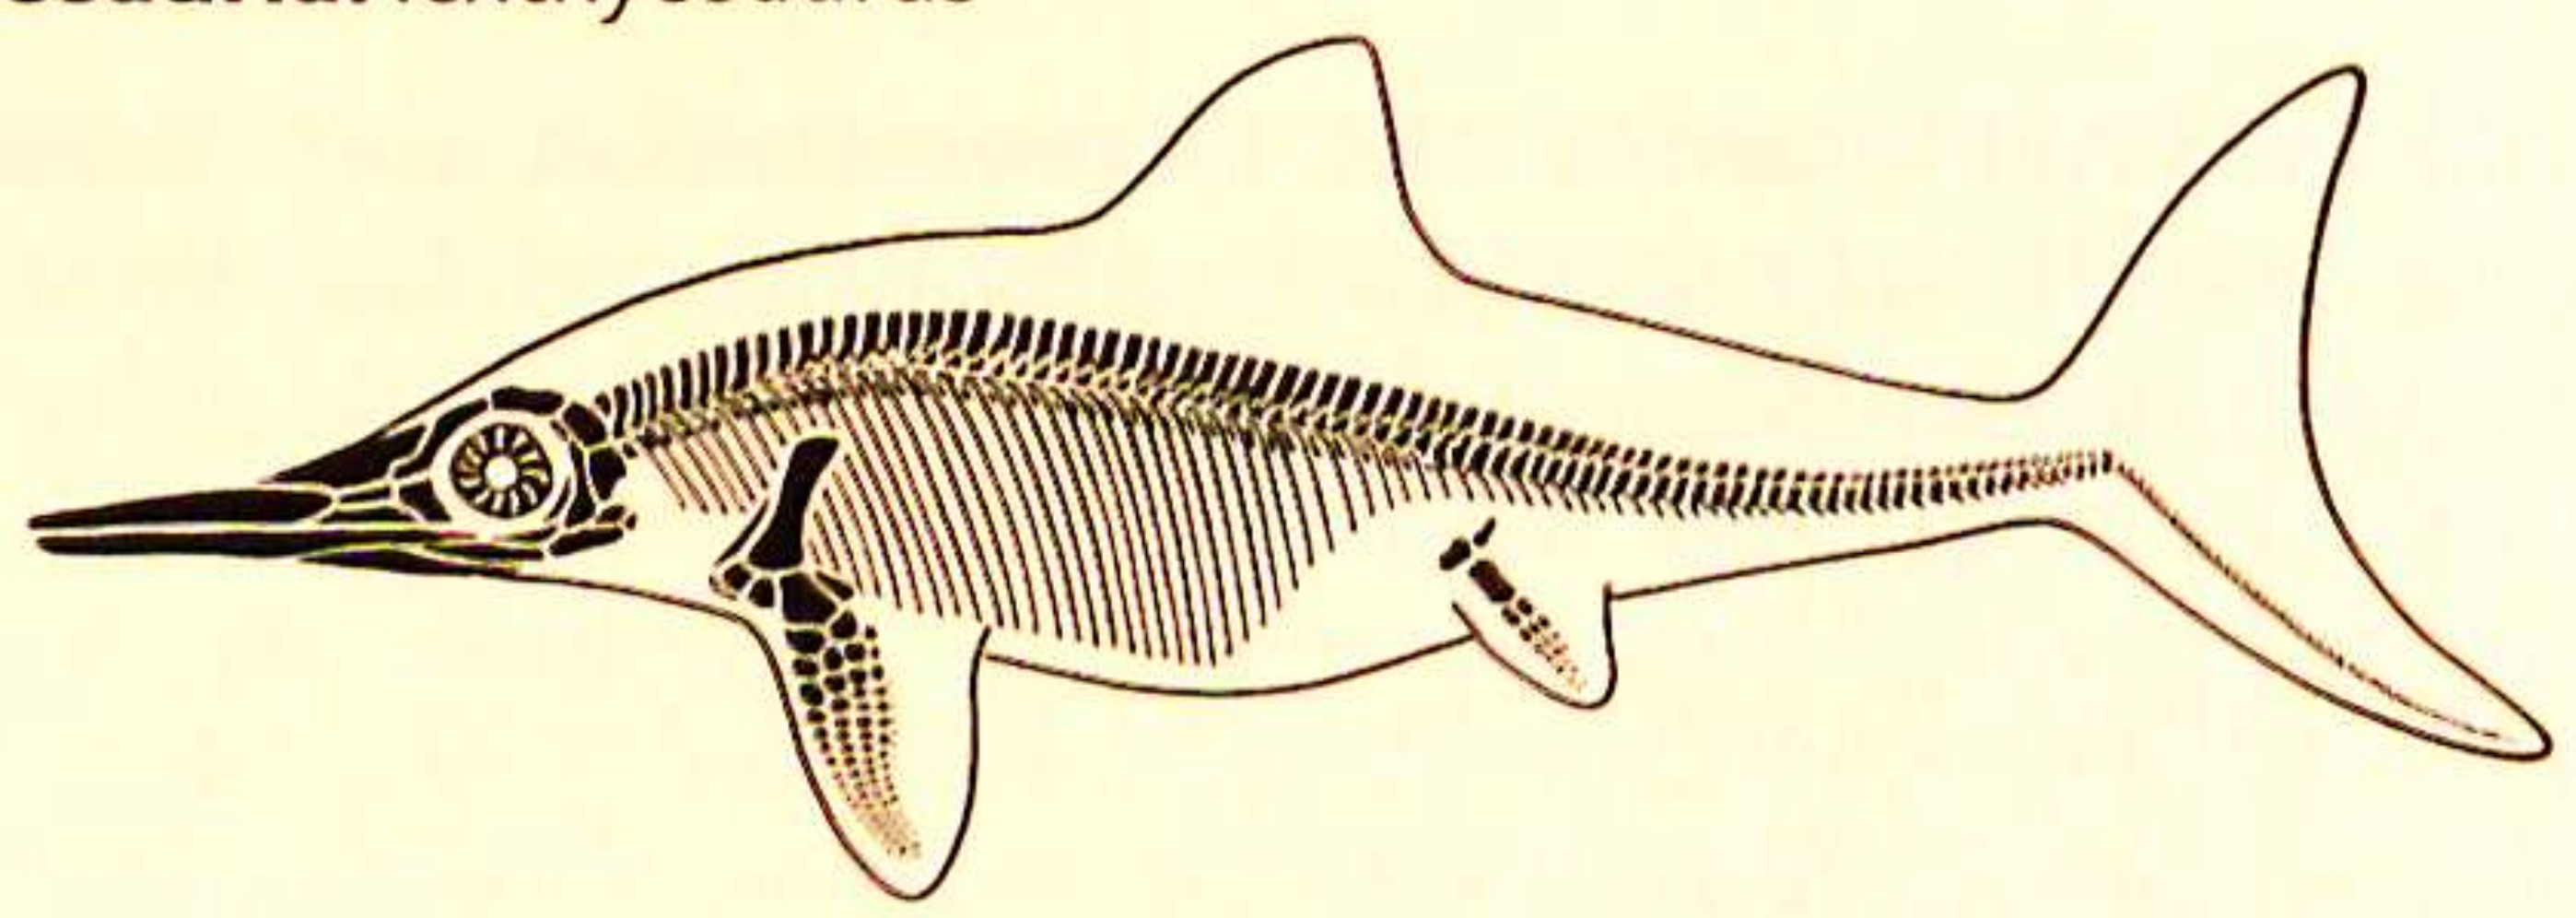
\includegraphics[width=0.2\textwidth]{../PCA/Skelettbilder_klein/Ichthyosaurus.jpg}}~
\subfloat[Ichthyostega]{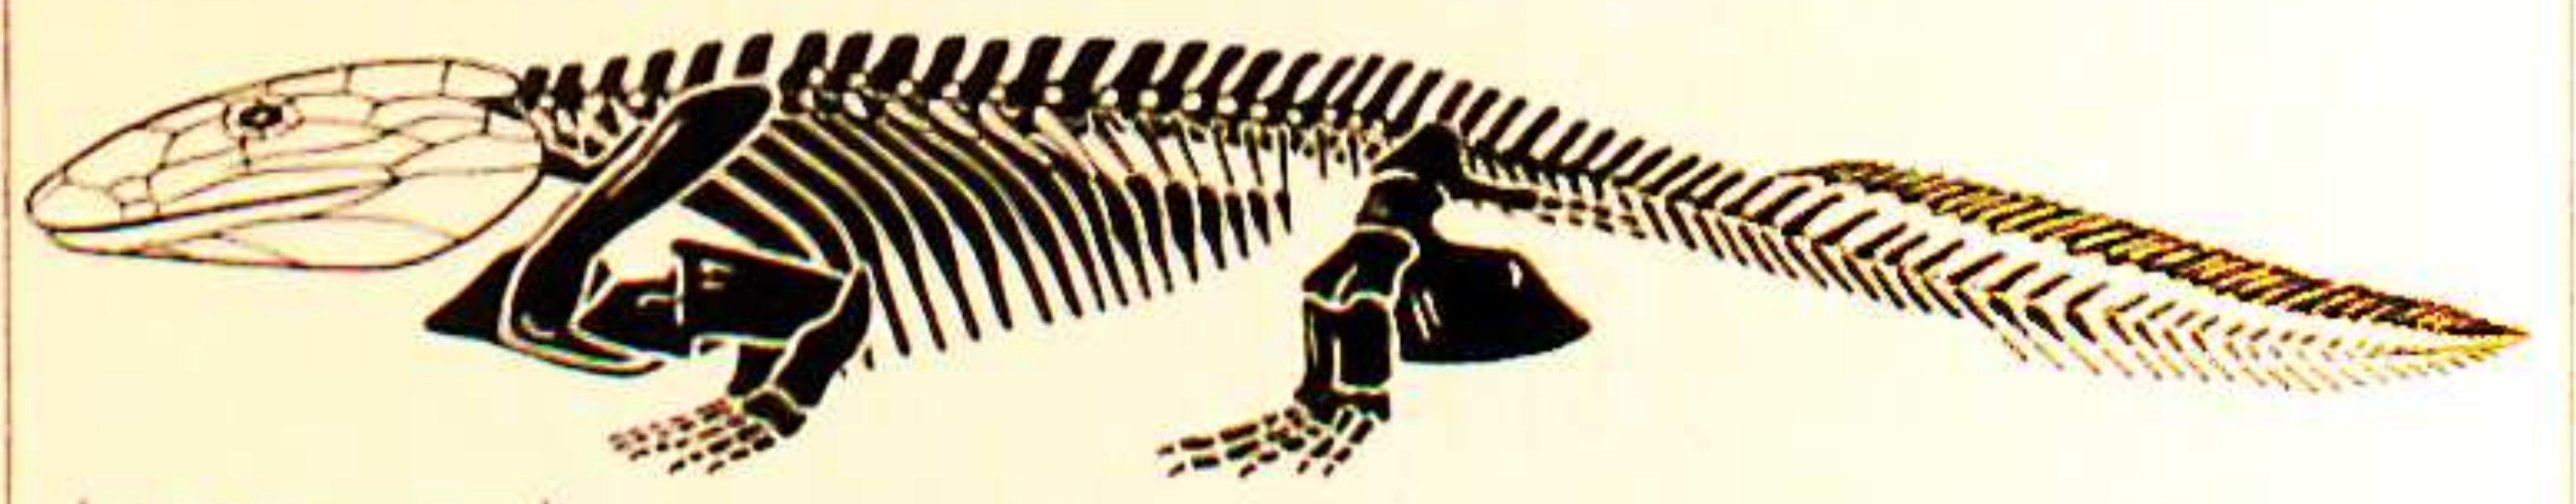
\includegraphics[width=0.2\textwidth]{../PCA/Skelettbilder_klein/Ichthyostega.jpg}}~
\subfloat[Känguru]{\includegraphics[width=0.2\textwidth]{../PCA/Skelettbilder_klein/Kaenguru.jpg}}~
\subfloat[Kaffernbüffel]{\includegraphics[width=0.2\textwidth]{../PCA/Skelettbilder_klein/Kaffernbueffel.jpg}}
\\
\subfloat[Kaninchen]{\includegraphics[width=0.2\textwidth]{../PCA/Skelettbilder_klein/Kaninchen.jpg}}~
\subfloat[Klippschliefer]{\includegraphics[width=0.2\textwidth]{../PCA/Skelettbilder_klein/Klippschliefer.jpg}}~
\subfloat[Koboldmaki]{\includegraphics[width=0.2\textwidth]{../PCA/Skelettbilder_klein/Koboldmaki.jpg}}~
\subfloat[Krokodil]{\includegraphics[width=0.2\textwidth]{../PCA/Skelettbilder_klein/Krokodil.jpg}}~
\subfloat[Landschildkröte]{\includegraphics[width=0.2\textwidth]{../PCA/Skelettbilder_klein/Landschildkroete.jpg}}
\phantomcaption

\end{figure}
\begin{figure}
\ContinuedFloat

\subfloat[Ohrenrobbe]{\includegraphics[width=0.2\textwidth]{../PCA/Skelettbilder_klein/Ohrenrobbe.jpg}}~
\subfloat[Panzerspitzmaus]{\includegraphics[width=0.2\textwidth]{../PCA/Skelettbilder_klein/Panzerspitzmaus.jpg}}~
\subfloat[Parasaurolophus walkeri]{\includegraphics[width=0.2\textwidth]{../PCA/Skelettbilder_klein/Parasaurolophus_walkeri.jpg}}~
\subfloat[Peloneustes philarchus]{\includegraphics[width=0.2\textwidth]{../PCA/Skelettbilder_klein/Peloneustes_philarchus.jpg}}~
\subfloat[Pferd]{\includegraphics[width=0.2\textwidth]{../PCA/Skelettbilder_klein/Pferd.jpg}}
\\
\subfloat[Pottwal]{\includegraphics[width=0.2\textwidth]{../PCA/Skelettbilder_klein/Pottwal.jpg}}~
\subfloat[Rothirsch]{\includegraphics[width=0.2\textwidth]{../PCA/Skelettbilder_klein/Rothirsch.jpg}}~
\subfloat[Schwan]{\includegraphics[width=0.2\textwidth]{../PCA/Skelettbilder_klein/Schwan.jpg}}~
\subfloat[Schwein]{\includegraphics[width=0.2\textwidth]{../PCA/Skelettbilder_klein/Schwein.jpg}}~
\subfloat[Seehund]{\includegraphics[width=0.2\textwidth]{../PCA/Skelettbilder_klein/Seehund.jpg}}
\\
\subfloat[Sinornis]{\includegraphics[width=0.2\textwidth]{../PCA/Skelettbilder_klein/Sinornis.jpg}}~
\subfloat[Stegosaurus]{\includegraphics[width=0.2\textwidth]{../PCA/Skelettbilder_klein/Stegosaurus.jpg}}~
\subfloat[Strauss]{\includegraphics[width=0.2\textwidth]{../PCA/Skelettbilder_klein/Strauss.jpg}}~
\subfloat[Taube]{\includegraphics[width=0.2\textwidth]{../PCA/Skelettbilder_klein/Taube.jpg}}~
\subfloat[Thrinaxodon]{\includegraphics[width=0.2\textwidth]{../PCA/Skelettbilder_klein/Thrinaxodon.jpg}}
\\
\subfloat[Triceratops]{\includegraphics[width=0.2\textwidth]{../PCA/Skelettbilder_klein/Triceratops.jpg}}~
\subfloat[Tyrannosaurus Rex]{\includegraphics[width=0.2\textwidth]{../PCA/Skelettbilder_klein/Tyrannosaurus_Rex.jpg}}~
\subfloat[Urpferdchen]{\includegraphics[width=0.2\textwidth]{../PCA/Skelettbilder_klein/Urpferdchen.jpg}}


\caption{Alle Bilder, die als Eingabe für die PCA verwendet wurden.}
\label{all_images}
\end{figure}


 
 \subsection{Gewichte}
 \label{appendix_pca_weight}
 
 \begin{itemize}
  \item Afrikanischer Elefant 4000kg, \url{https://de.upali.ch/gewicht-und-grosse/}
  \item Afrikanischer Strauß bis 135kg, \url{https://de.wikipedia.org/wiki/Afrikanischer_Strau\%C3\%9F}
  \item Amerikanischer Flussbarsch 2kg, \url{http://tierdoku.com/index.php?title=Amerikanischer_Flussbarsch}
  \item Archaeopteryx 1kg, \url{https://de.wikipedia.org/wiki/Archaeopteryx}
  \item Blauwal 120 Tonnen, \url{http://tierdoku.com/index.php?title=Blauwal}, "`das schwerste bekannte Tier der Erdgeschichte"' \url{https://de.wikipedia.org/wiki/Blauwal}
  \item Brachiosaurus 23-44 Tonnen, \url{https://de.wikipedia.org/wiki/Brachiosaurus}
  \item Chamäleon 0,1-2kg, \url{https://www.tierchenwelt.de/echsen/128-chamaeleon.html}
  \item Dimetrodon 250kg, \url{https://de.wikipedia.org/wiki/Dimetrodon}
  \item Dromedar 300-700kg, \url{https://de.wikipedia.org/wiki/Dromedar}
  \item Durschnittsgewicht (Warmblut-)Pferd 600 kg, \url{https://www.reitarena.com/de/blog/blog-post/2015/03/03/das-pferd-grundlegende-fakten.html}
  \item Elster 0,2kg, \url{https://de.wikipedia.org/wiki/Elster}
  \item Forelle 10-50kg (je nach Art), \url{https://de.wikipedia.org/wiki/Forelle}
  \item Frosch 10g, \url{http://www.biologie-schule.de/frosch-steckbrief.php}
  \item Gämse 25-50kg, \url{https://de.wikipedia.org/wiki/G\%C3\%A4mse}
  \item Girafffe bis 2 Tonnen, \url{https://www.tierchenwelt.de/huftiere/73-giraffe.html}
  \item Gnu 140-250kg, \url{https://de.wikipedia.org/wiki/Gnus}
  \item Grönlandwal 50-100 Tonnen, \url{https://de.wikipedia.org/wiki/Gr\%C3\%B6nlandwal}
  \item Ichthyornis 0.3kg, \url{http://dinodata.de/animals/birds/pages_i/ichthyornis.php}
  \item Ichthyosaurus 90kg, \url{https://www.tiere-online.de/sonstige-tiere/dinosaurier/ichthyosaurus/}
  \item Ichthyostega 80kg, \url{https://dinosaurierwelt.com/ichthyostega/}
  \item Kaffernbüffel 350-900kg, \url{https://de.wikipedia.org/wiki/Kaffernb\%C3\%BCffel}
  \item Känguru 2-90kg ,\url{https://de.wikipedia.org/wiki/K\%C3\%A4ngurus}
  \item Kaninchen je nach Art, ganz grob 1kg
  \item Klippschliefer 2-5kg, \url{https://de.wikipedia.org/wiki/Klippschliefer}
  \item Koboldmaki 0,1kg, \url{https://de.wikipedia.org/wiki/Koboldmakis}
  \item Krokodil 100-1000kg, \url{https://de.wikipedia.org/wiki/Krokodile}
  \item Landschildkröte je nach Art, grob 50kg
  \item Ohrenrobbe 25-500kg, \url{https://de.wikipedia.org/wiki/Ohrenrobben}
  \item Panzerspitzmaus 100g ,\url{https://de.wikipedia.org/wiki/Panzerspitzmaus}
  \item Parasaurolophus walkeri 4-5 Tonnen, \url{http://tierdoku.com/index.php?title=Parasaurolophus_walkeri}
  \item Peloneustes philarchus 100kg, \url{https://de.wikipedia.org/wiki/Peloneustes}
  \item Pottwal bis 50 Tonnen, \url{https://de.wikipedia.org/wiki/Pottwal}
  \item Rothirsch 80-350kg, \url{https://de.wikipedia.org/wiki/Rothirsch}
  \item Schlange bis 100kg bei Riesenschlangen, \url{https://de.wikipedia.org/wiki/Schlangen}
  \item Schwan 14kg, \url{https://de.wikipedia.org/wiki/Schw\%C3\%A4ne}
  \item Schwein 100kg, \url{https://de.wikipedia.org/wiki/Hausschwein}
  \item Seehund 100-150kg, \url{https://de.wikipedia.org/wiki/Seehund}
  \item Sinornis 20g, \url{http://dinodata.de/animals/birds/pages_s/sinornis.php}
  \item Stegosaurus 4,5 Tonnen, \url{https://de.wikipedia.org/wiki/Stegosaurus}
  \item Taube je nach Art, grob 1-2kg
  \item Thrinaxodon Reptil "`ein paar Pfund"', \url{https://www.thoughtco.com/thrinaxodon-1091887}
  \item Triceratops 6-12 Tonnen, \url{https://de.wikipedia.org/wiki/Triceratops}
  \item Tyrannosaurus 9 Tonnen, \url{https://de.wikipedia.org/wiki/Tyrannosaurus}
  \item Urpferdchen (Propalaeotherium) 30kg, \url{https://de.wikipedia.org/wiki/Propalaeotherium}
 \end{itemize}
 

% --------------
% Erhobene Werte
% --------------

  \begin{figure}
   \subfloat[Erster Punkt des Halses]{\includegraphics[width=0.3\textwidth]{../PCA/gnuplot/results_with_leg_tag/input_neck1.pdf}}
   \qquad
   \subfloat[Zweiter Punkt des Halses]{\includegraphics[width=0.3\textwidth]{../PCA/gnuplot/results_with_leg_tag/input_neck2.pdf}}
   \qquad
   \subfloat[Dritter Punkt des Halses]{\includegraphics[width=0.3\textwidth]{../PCA/gnuplot/results_with_leg_tag/input_neck3.pdf}}
   \\
   \subfloat[Vierter Punkt des Halses \bzw erster Punkt des Rückens]{\includegraphics[width=0.3\textwidth]{../PCA/gnuplot/results_with_leg_tag/input_back1.pdf}}
   \qquad
   \subfloat[Zweiter Punkt des Rückens]{\includegraphics[width=0.3\textwidth]{../PCA/gnuplot/results_with_leg_tag/input_back2.pdf}}
   \qquad
   \subfloat[Dritter Punkt des Rückens]{\includegraphics[width=0.3\textwidth]{../PCA/gnuplot/results_with_leg_tag/input_back3.pdf}}
   \\
   \subfloat[Vierter Punkt des Rückens \bzw erster Punkt des Schwanzes]{\includegraphics[width=0.3\textwidth]{../PCA/gnuplot/results_with_leg_tag/input_back4.pdf}}
   \qquad
   \subfloat[Zweiter Punkt des Schwanzes]{\includegraphics[width=0.3\textwidth]{../PCA/gnuplot/results_with_leg_tag/input_tail2.pdf}}
   \qquad
   \subfloat[Dritter Punkt des Schwanzes]{\includegraphics[width=0.3\textwidth]{../PCA/gnuplot/results_with_leg_tag/input_tail3.pdf}}
   \\
   \subfloat[Vierter Punkt des Schwanzes]{\includegraphics[width=0.3\textwidth]{../PCA/gnuplot/results_with_leg_tag/input_tail4.pdf}}
   \qquad
   \subfloat[Länge Ober- und Unterarm]{\includegraphics[width=0.3\textwidth]{../PCA/gnuplot/results_with_leg_tag/input_upper+lowerArm.pdf}}
   \qquad
   \subfloat[Länge Unterarm und Hand]{\includegraphics[width=0.3\textwidth]{../PCA/gnuplot/results_with_leg_tag/input_lowerArm+hand.pdf}}
   \phantomcaption
  \end{figure}
  \begin{figure}
   \ContinuedFloat
   \subfloat[Länge Ober- und Unterschenkel]{\includegraphics[width=0.3\textwidth]{../PCA/gnuplot/results_with_leg_tag/input_upper+lowerLeg.pdf}}
   \qquad
   \subfloat[Länge Unterschenkel und Fuß]{\includegraphics[width=0.3\textwidth]{../PCA/gnuplot/results_with_leg_tag/input_lowerLeg+foot.pdf}}
   
   \caption{Erhobene Daten: Punkte der Bézierkurven der Wirbelsäule und Längen der Extremitäten. Bei den Extremitäten ist jeweils gegeneinander abgetragen Ober- und Unterarm, Ober- und Unterschenkel, Unterarm und Hand, Unterschenkel und Fuß. Markiert ist jeweils ob die Datenpunkte $0$ (rot), $2$ (blau) oder $4$ (grün) Beine haben.}
   \label{input_data}
  \end{figure}
  
 \begin{figure}
  \subfloat[lineare Skala]{\includegraphics[width=0.5\textwidth]{../PCA/gnuplot/results_with_leg_tag/input_weight.pdf} \label{gnuplot_weight}}
  \qquad
  \subfloat[logarithmische Skala]{\includegraphics[width=0.5\textwidth]{../PCA/gnuplot/results_with_leg_tag/input_weight_logarithmic.pdf}\label{gnuplot_log_weight}}
  
  \caption{Erhobene Daten: Gewicht. Markiert ist jeweils ob die Datenpunkte $0$ (rot), $2$ (blau) oder $4$ (grün) Beine haben.}
  \label{input_data_weight}
 \end{figure}
 
 %--------------
 % QQ Diagramme
 % ------------

  \begin{figure}
   \subfloat[Erster Punkt des Halses, x-Koordinate]{\includegraphics[width=0.3\textwidth]{../PCA/gnuplot/results_qq_diagrams/QQ_diagram0.pdf}}
   \qquad
   \subfloat[Erster Punkt des Halses, y-Koordinate]{\includegraphics[width=0.3\textwidth]{../PCA/gnuplot/results_qq_diagrams/QQ_diagram1.pdf}}
   \qquad
   \subfloat[Zweiter Punkt des Halses, x-Koordinate]{\includegraphics[width=0.3\textwidth]{../PCA/gnuplot/results_qq_diagrams/QQ_diagram2.pdf}}
   \\
   \subfloat[Zweiter Punkt des Halses, y-Koordinate]{\includegraphics[width=0.3\textwidth]{../PCA/gnuplot/results_qq_diagrams/QQ_diagram3.pdf}}
   \qquad
   \subfloat[Dritter Punkt des Halses, x-Koordinate]{\includegraphics[width=0.3\textwidth]{../PCA/gnuplot/results_qq_diagrams/QQ_diagram4.pdf}}
   \qquad
   \subfloat[Dritter Punkt des Halses, y-Koordinate]{\includegraphics[width=0.3\textwidth]{../PCA/gnuplot/results_qq_diagrams/QQ_diagram5.pdf}}
   \\
   \subfloat[Erster Punkt des Rückens, x-Koordinate]{\includegraphics[width=0.3\textwidth]{../PCA/gnuplot/results_qq_diagrams/QQ_diagram6.pdf}}
   \qquad
   \subfloat[Erster Punkt des Rückens, y-Koordinate]{\includegraphics[width=0.3\textwidth]{../PCA/gnuplot/results_qq_diagrams/QQ_diagram7.pdf}}
   \qquad
   \subfloat[Zweiter Punkt des Rückens, x-Koordinate]{\includegraphics[width=0.3\textwidth]{../PCA/gnuplot/results_qq_diagrams/QQ_diagram8.pdf}}
   \\
   \subfloat[Zweiter Punkt des Rückens, y-Koordinate]{\includegraphics[width=0.3\textwidth]{../PCA/gnuplot/results_qq_diagrams/QQ_diagram9.pdf}}
   \qquad
   \subfloat[Dritter Punkt des Rückens, x-Koordinate]{\includegraphics[width=0.3\textwidth]{../PCA/gnuplot/results_qq_diagrams/QQ_diagram10.pdf}}
   \qquad
   \subfloat[Dritter Punkt des Rückens, y-Koordinate]{\includegraphics[width=0.3\textwidth]{../PCA/gnuplot/results_qq_diagrams/QQ_diagram11.pdf}}
   \phantomcaption
  \end{figure}
  \begin{figure}
   \ContinuedFloat
   \subfloat[Vierter Punkt des Rückens, x-Koordinate]{\includegraphics[width=0.3\textwidth]{../PCA/gnuplot/results_qq_diagrams/QQ_diagram12.pdf}}
   \qquad
   \subfloat[Vierter Punkt des Rückens, y-Koordinate]{\includegraphics[width=0.3\textwidth]{../PCA/gnuplot/results_qq_diagrams/QQ_diagram13.pdf}}
   \qquad
   \subfloat[Zweiter Punkt des Schwanzes, x-Koordinate]{\includegraphics[width=0.3\textwidth]{../PCA/gnuplot/results_qq_diagrams/QQ_diagram14.pdf}}
   \\
   \subfloat[Zweiter Punkt des Schwanzes, y-Koordinate]{\includegraphics[width=0.3\textwidth]{../PCA/gnuplot/results_qq_diagrams/QQ_diagram15.pdf}}
   \qquad
   \subfloat[Dritter Punkt des Schwanzes, x-Koordinate]{\includegraphics[width=0.3\textwidth]{../PCA/gnuplot/results_qq_diagrams/QQ_diagram16.pdf}}
   \qquad
   \subfloat[Dritter Punkt des Schwanzes, y-Koordinate]{\includegraphics[width=0.3\textwidth]{../PCA/gnuplot/results_qq_diagrams/QQ_diagram17.pdf}}
   \\
   \subfloat[Vierter Punkt des Schwanzes, x-Koordinate]{\includegraphics[width=0.3\textwidth]{../PCA/gnuplot/results_qq_diagrams/QQ_diagram18.pdf}}
   \qquad
   \subfloat[Vierter Punkt des Schwanzes, y-Koordinate]{\includegraphics[width=0.3\textwidth]{../PCA/gnuplot/results_qq_diagrams/QQ_diagram19.pdf}}
   
   \caption{Quantil-Quantil-Diagramme für alle Dimensionen der Wirbelsäule}
   \label{qq_diagrams_spine}
  \end{figure}
  \begin{figure}
   \subfloat[Länge Oberarm]{\includegraphics[width=0.3\textwidth]{../PCA/gnuplot/results_qq_diagrams/QQ_diagram22.pdf}}
   \qquad
   \subfloat[Länge Unterarm]{\includegraphics[width=0.3\textwidth]{../PCA/gnuplot/results_qq_diagrams/QQ_diagram23.pdf}}
   \qquad
   \subfloat[Länge Hand]{\includegraphics[width=0.3\textwidth]{../PCA/gnuplot/results_qq_diagrams/QQ_diagram24.pdf}}
   \\
   \subfloat[Länge Oberschenkel]{\includegraphics[width=0.3\textwidth]{../PCA/gnuplot/results_qq_diagrams/QQ_diagram25.pdf}}
   \qquad
   \subfloat[Länge Unterschenkel]{\includegraphics[width=0.3\textwidth]{../PCA/gnuplot/results_qq_diagrams/QQ_diagram26.pdf}}
   \qquad
   \subfloat[Länge Fuß]{\includegraphics[width=0.3\textwidth]{../PCA/gnuplot/results_qq_diagrams/QQ_diagram27.pdf}}

   \caption{Quantil-Quantil-Diagramme für die Dimensionen der Eingabedaten, die zusätzlich zur Wirbelsäule erhoben wurden. Nicht dargestellt ist das binäre Attribut \emph{Flügel} und die Anzahl der Beine mit Bodenkontakt.}
   \label{qq_diagrams_rest}
  \end{figure}
  
  
% ----------------------------
% Mit PCA erzeugte Datenpunkte
% ----------------------------
 
 \begin{figure}
   \centering
   \subfloat[1-, \emph{Flügel} $0,38$, \emph{Beine} $1,6$, \emph{Gewicht} $92$kg]{\includegraphics[width=0.45\textwidth]{../PCA/sqrtEV_log_weight_downscaled_wings_legs_and_weight/EV1_neg.jpg}}
   \qquad
   \subfloat[1+, \emph{Flügel} $-0,057$, \emph{Beine} $1,2$, \emph{Gewicht} $94$kg]{\includegraphics[width=0.45\textwidth]{../PCA/sqrtEV_log_weight_downscaled_wings_legs_and_weight/EV1_pos.jpg}}
   \\
   \subfloat[2-, \emph{Flügel} $0,014$, \emph{Beine} $1,4$, \emph{Gewicht} $94$kg]{\includegraphics[width=0.45\textwidth]{../PCA/sqrtEV_log_weight_downscaled_wings_legs_and_weight/EV2_neg.jpg}}
   \qquad
   \subfloat[2+, \emph{Flügel} $0,3$, \emph{Beine} $1,3$, \emph{Gewicht} $93$kg]{\includegraphics[width=0.45\textwidth]{../PCA/sqrtEV_log_weight_downscaled_wings_legs_and_weight/EV2_pos.jpg}}
   \\
   \subfloat[3-, \emph{Flügel} $0,11$, \emph{Beine} $1,6$, \emph{Gewicht} $93$kg]{\includegraphics[width=0.45\textwidth]{../PCA/sqrtEV_log_weight_downscaled_wings_legs_and_weight/EV3_neg.jpg}}
   \qquad
   \subfloat[3+, \emph{Flügel} $0,21$, \emph{Beine} $1,2$, \emph{Gewicht} $93$kg]{\includegraphics[width=0.45\textwidth]{../PCA/sqrtEV_log_weight_downscaled_wings_legs_and_weight/EV3_pos.jpg}}
   \phantomcaption
 \end{figure}
 \begin{figure}
   \ContinuedFloat
   \centering
   \subfloat[4-, \emph{Flügel} $0,3$, \emph{Beine} $1$, \emph{Gewicht} $92$kg]{\includegraphics[width=0.45\textwidth]{../PCA/sqrtEV_log_weight_downscaled_wings_legs_and_weight/EV4_neg.jpg}}
   \qquad
   \subfloat[4+, \emph{Flügel} $0,022$, \emph{Beine} $1,8$, \emph{Gewicht} $94$kg]{\includegraphics[width=0.45\textwidth]{../PCA/sqrtEV_log_weight_downscaled_wings_legs_and_weight/EV4_pos.jpg}}
   \\
   \subfloat[5-, \emph{Flügel} $0,08$, \emph{Beine} $1,6$, \emph{Gewicht} $93$kg]{\includegraphics[width=0.45\textwidth]{../PCA/sqrtEV_log_weight_downscaled_wings_legs_and_weight/EV5_neg.jpg}}
   \qquad
   \subfloat[5+, \emph{Flügel} $0,24$, \emph{Beine} $1,2$, \emph{Gewicht} $93$kg]{\includegraphics[width=0.45\textwidth]{../PCA/sqrtEV_log_weight_downscaled_wings_legs_and_weight/EV5_pos.jpg}}
   \\
   \subfloat[6-, \emph{Flügel} $0,21$, \emph{Beine} $1,5$, \emph{Gewicht} $92$kg]{\includegraphics[width=0.45\textwidth]{../PCA/sqrtEV_log_weight_downscaled_wings_legs_and_weight/EV6_neg.jpg}}
   \qquad
   \subfloat[6+, \emph{Flügel} $0,11$, \emph{Beine} $1,3$, \emph{Gewicht} $98$kg]{\includegraphics[width=0.45\textwidth]{../PCA/sqrtEV_log_weight_downscaled_wings_legs_and_weight/EV6_pos.jpg}}
   
   \caption{Datenpunkte im PCA-Koordinatensystem. Eine Koordinate nimmt den Wert der positiven (+) \bzw negativen (-) Standardabweichung in die entsprechende Richtung an, alle anderen sind null. Von oben nach unten sind die Ergebnisse für den größten (1) bis zum sechstgrößten (6) Eigenwert dargestellt. \emph{Beine} steht für \emph{Beine mit Bodenkontakt}.}
   \label{pca_results_sqrtEV}
  \end{figure}

\end{appendices}

\Erklaerung
\end{document}
